%% \documentclass[18]{extarticle}
%% \usepackage{geometry}
%\documentclass[12]{article}
%%!TEX root = paper.tex
\usepackage{amssymb, amsmath, amsthm, mathtools,bbold}
\usepackage[utf8]{inputenc}

% Formatting

  % Page options
    \usepackage{geometry}
    \geometry{margin=1in}
    \usepackage{parskip}

  %% % Theorem styles, environments
  %%   \newtheoremstyle{spacedplain}
  %%     {\parskip}{0pt}{\itshape}{}{\bfseries}{.}{5pt plus 1pt minus 1pt}{}
  %%   \newtheoremstyle{spaceddefinition}
  %%     {\parskip}{0pt}{\normalfont}{}{\bfseries}{.}{5pt plus 1pt minus 1pt}{}
  %%   \newtheoremstyle{spacedremark}
  %%     {\parskip}{0pt}{\normalfont}{}{\itshape}{.}{5pt plus 1pt minus 1pt}{}

  %%   \theoremstyle{spacedplain}
  \usepackage{amsmath,amssymb,amscd}
\usepackage{amsfonts,graphicx,psfrag,esint}

\renewcommand{\Re}{\mathbb{R}}
\newcommand{\ds}{\displaystyle}

\newcommand{\half}{\frac{1}{2}}
\newcommand{\weak}{\rightharpoonup}
\newcommand{\embed}{\hookrightarrow}
\newcommand{\cembed}{\hookrightarrow \!\!\!\! \rightarrow}
%\newcommand{\ave}{\,-\!\!\!\!\!\!\!\int}
\newcommand{\ave}{\fint}
\newcommand{\vph}{\vphantom{A^{A}_{A}}}
\newcommand{\sst}{\,\mid\,}
\newcommand{\gap}{\hspace*{0.25in}}

\newcommand{\dbyd}[2]{\frac{d #1}{d #2}}
\newcommand{\dbydp}[2]{\frac{\partial #1}{\partial #2}}

\newcommand{\eqnref}[1]{(\ref{eqn#1})}

\newcommand{\ahat}{\hat{a}}
\newcommand{\bhat}{\hat{b}}
\newcommand{\chat}{\hat{c}}
\newcommand{\dhat}{\hat{d}}
\newcommand{\ehat}{\hat{e}}
\newcommand{\fhat}{\hat{f}}
\newcommand{\ghat}{\hat{g}}
\newcommand{\hhat}{\hat{h}}
\newcommand{\ihat}{\hat{i}}
\newcommand{\jhat}{\hat{j}}
\newcommand{\khat}{\hat{k}}
\newcommand{\lhat}{\hat{l}}
\newcommand{\ellhat}{\hat{\ell}}
\newcommand{\mhat}{\hat{m}}
\newcommand{\nhat}{\hat{n}}
\newcommand{\ohat}{\hat{o}}
\newcommand{\phat}{\hat{p}}
\newcommand{\qhat}{\hat{q}}
\newcommand{\rhat}{\hat{r}}
\newcommand{\shat}{\hat{s}}
\newcommand{\that}{\hat{t}}
\newcommand{\uhat}{\hat{u}}
\newcommand{\vhat}{\hat{v}}
\newcommand{\what}{\hat{w}}
\newcommand{\xhat}{\hat{x}}
\newcommand{\yhat}{\hat{y}}
\newcommand{\zhat}{\hat{z}}

\newcommand{\Ahat}{\hat{A}}
\newcommand{\Bhat}{\hat{B}}
\newcommand{\Chat}{\hat{C}}
\newcommand{\Dhat}{\hat{D}}
\newcommand{\Ehat}{\hat{E}}
\newcommand{\Fhat}{\hat{F}}
\newcommand{\Ghat}{\hat{G}}
\newcommand{\Hhat}{\hat{H}}
\newcommand{\Ihat}{\hat{I}}
\newcommand{\Jhat}{\hat{J}}
\newcommand{\Khat}{\hat{K}}
\newcommand{\Lhat}{\hat{L}}
\newcommand{\Mhat}{\hat{M}}
\newcommand{\Nhat}{\hat{N}}
\newcommand{\Ohat}{\hat{O}}
\newcommand{\Phat}{\hat{P}}
\newcommand{\Qhat}{\hat{Q}}
\newcommand{\Rhat}{\hat{R}}
\newcommand{\Shat}{\hat{S}}
\newcommand{\That}{\hat{T}}
\newcommand{\Uhat}{\hat{U}}
\newcommand{\Vhat}{\hat{V}}
\newcommand{\What}{\hat{W}}
\newcommand{\Xhat}{\hat{X}}
\newcommand{\Yhat}{\hat{Y}}
\newcommand{\Zhat}{\hat{Z}}

\newcommand{\alphahat}{\hat{\alpha}}
\newcommand{\betahat}{\hat{\beta}}
\newcommand{\gammahat}{\hat{\gamma}}
\newcommand{\deltahat}{\hat{\delta}}
\newcommand{\epsilinhat}{\hat{\epsilon}}
\newcommand{\varepsilinhat}{\hat{\varepsilon}}
\newcommand{\zetahat}{\hat{\zeta}}
\newcommand{\etahat}{\hat{\eta}}
\newcommand{\thetahat}{\hat{\theta}}
\newcommand{\varthetahat}{\hat{\vartheta}}
\newcommand{\iotahat}{\hat{\iota}}
\newcommand{\kappahat}{\hat{\kappa}}
\newcommand{\lambdahat}{\hat{\lambda}}
\newcommand{\muhat}{\hat{\mu}}
\newcommand{\nuhat}{\hat{\nu}}
\newcommand{\xihat}{\hat{\xi}}
\newcommand{\pihat}{\hat{\pi}}
\newcommand{\varpihat}{\hat{\varpi}}
\newcommand{\rhohat}{\hat{\rho}}
\newcommand{\varrhohat}{\hat{\varrho}}
\newcommand{\sigmahat}{\hat{\sigma}}
\newcommand{\varsigmahat}{\hat{\varsigma}}
\newcommand{\tauhat}{\hat{\tau}}
\newcommand{\upsilonhat}{\hat{\upsilon}}
\newcommand{\phihat}{\hat{\phi}}
\newcommand{\varphihat}{\hat{\varphi}}
\newcommand{\chihat}{\hat{\chi}}
\newcommand{\psihat}{\hat{\psi}}
\newcommand{\omegahat}{\hat{\omega}}

\newcommand{\Gammahat}{\hat{\Gamma}}
\newcommand{\Deltahat}{\hat{\Delta}}
\newcommand{\Thetahat}{\hat{\Theta}}
\newcommand{\Lambdahat}{\hat{\Lambda}}
\newcommand{\Xihat}{\hat{\Xi}}
\newcommand{\Pihat}{\hat{\Pi}}
\newcommand{\Sigmahat}{\hat{\Sigma}}
\newcommand{\Upsilonhat}{\hat{\Upsilon}}
\newcommand{\Phihat}{\hat{\Phi}}
\newcommand{\Psihat}{\hat{\Psi}}
\newcommand{\Omegahat}{\hat{\Omega}}

\newcommand{\bba}{\mathbb{a}}
\newcommand{\bbb}{\mathbb{b}}
\newcommand{\bbc}{\mathbb{c}}
\newcommand{\bbd}{\mathbb{d}}
\newcommand{\bbe}{\mathbb{e}}
\newcommand{\bbf}{\mathbb{f}}
\newcommand{\bbg}{\mathbb{g}}
\newcommand{\bbh}{\mathbb{h}}
\newcommand{\bbi}{\mathbb{i}}
\newcommand{\bbj}{\mathbb{j}}
\newcommand{\bbk}{\mathbb{k}}
\newcommand{\bbl}{\mathbb{l}}
\newcommand{\bbm}{\mathbb{m}}
\newcommand{\bbn}{\mathbb{n}}
\newcommand{\bbo}{\mathbb{o}}
\newcommand{\bbp}{\mathbb{p}}
\newcommand{\bbq}{\mathbb{q}}
\newcommand{\bbr}{\mathbb{r}}
\newcommand{\bbs}{\mathbb{s}}
\newcommand{\bbt}{\mathbb{t}}
\newcommand{\bbu}{\mathbb{u}}
\newcommand{\bbv}{\mathbb{v}}
\newcommand{\bbw}{\mathbb{w}}
\newcommand{\bbx}{\mathbb{x}}
\newcommand{\bby}{\mathbb{y}}
\newcommand{\bbz}{\mathbb{z}}

\newcommand{\bbA}{\mathbb{A}}
\newcommand{\bbB}{\mathbb{B}}
\newcommand{\bbC}{\mathbb{C}}
\newcommand{\bbD}{\mathbb{D}}
\newcommand{\bbE}{\mathbb{E}}
\newcommand{\bbF}{\mathbb{F}}
\newcommand{\bbG}{\mathbb{G}}
\newcommand{\bbH}{\mathbb{H}}
\newcommand{\bbI}{\mathbb{I}}
\newcommand{\bbJ}{\mathbb{J}}
\newcommand{\bbK}{\mathbb{K}}
\newcommand{\bbL}{\mathbb{L}}
\newcommand{\bbM}{\mathbb{M}}
\newcommand{\bbN}{\mathbb{N}}
\newcommand{\bbO}{\mathbb{O}}
\newcommand{\bbP}{\mathbb{P}}
\newcommand{\bbQ}{\mathbb{Q}}
\newcommand{\bbR}{\mathbb{R}}
\newcommand{\bbS}{\mathbb{S}}
\newcommand{\bbT}{\mathbb{T}}
\newcommand{\bbU}{\mathbb{U}}
\newcommand{\bbV}{\mathbb{V}}
\newcommand{\bbW}{\mathbb{W}}
\newcommand{\bbX}{\mathbb{X}}
\newcommand{\bbY}{\mathbb{Y}}
\newcommand{\bbZ}{\mathbb{Z}}

\newcommand{\abar}{{\bar{a}}}
\newcommand{\bbar}{{\bar{b}}}
\newcommand{\cbar}{{\bar{c}}}
\newcommand{\dbar}{{\bar{d}}}
\newcommand{\ebar}{{\bar{e}}}
\newcommand{\fbar}{{\bar{f}}}
\newcommand{\gbar}{{\bar{g}}}
\newcommand{\barh}{{\bar{h}}}
\newcommand{\ibar}{{\bar{i}}}
\newcommand{\jbar}{{\bar{j}}}
\newcommand{\kbar}{{\bar{k}}}
\newcommand{\lbar}{{\bar{l}}}
\newcommand{\mbar}{{\bar{m}}}
\newcommand{\nbar}{{\bar{n}}}
% \newcommand{\obar}{{\bar{o}}}
\newcommand{\pbar}{{\bar{p}}}
\newcommand{\qbar}{{\bar{q}}}
\newcommand{\rbar}{{\bar{r}}}
\newcommand{\sbar}{{\bar{s}}}
\newcommand{\tbar}{{\bar{t}}}
\newcommand{\ubar}{{\bar{u}}}
\newcommand{\vbar}{{\bar{v}}}
\newcommand{\wbar}{{\bar{w}}}
\newcommand{\xbar}{{\bar{x}}}
\newcommand{\ybar}{{\bar{y}}}
\newcommand{\zbar}{{\bar{z}}}

\newcommand{\Abar}{{\bar{A}}}
\newcommand{\Bbar}{{\bar{B}}}
\newcommand{\Cbar}{{\bar{C}}}
\newcommand{\Dbar}{{\bar{D}}}
\newcommand{\Ebar}{{\bar{E}}}
\newcommand{\Fbar}{{\bar{F}}}
\newcommand{\Gbar}{{\bar{G}}}
\newcommand{\Hbar}{{\bar{H}}}
\newcommand{\Ibar}{{\bar{I}}}
\newcommand{\Jbar}{{\bar{J}}}
\newcommand{\Kbar}{{\bar{K}}}
\newcommand{\Lbar}{{\bar{L}}}
\newcommand{\Mbar}{{\bar{M}}}
\newcommand{\Nbar}{{\bar{N}}}
\newcommand{\Obar}{{\bar{O}}}
\newcommand{\Pbar}{{\bar{P}}}
\newcommand{\Qbar}{{\bar{Q}}}
\newcommand{\Rbar}{{\bar{R}}}
\newcommand{\Sbar}{{\bar{S}}}
\newcommand{\Tbar}{{\bar{T}}}
\newcommand{\Ubar}{{\bar{U}}}
\newcommand{\Vbar}{{\bar{V}}}
\newcommand{\Wbar}{{\bar{W}}}
\newcommand{\Xbar}{{\bar{X}}}
\newcommand{\Ybar}{{\bar{Y}}}
\newcommand{\Zbar}{{\bar{Z}}}

\newcommand{\alphabar}{\bar{\alpha}}
\newcommand{\betabar}{\bar{\beta}}
\newcommand{\gammabar}{\bar{\gamma}}
\newcommand{\deltabar}{\bar{\delta}}
\newcommand{\epsilinbar}{\bar{\epsilon}}
\newcommand{\varepsilinbar}{\bar{\varepsilon}}
\newcommand{\zetabar}{\bar{\zeta}}
\newcommand{\etabar}{\bar{\eta}}
\newcommand{\thetabar}{\bar{\theta}}
\newcommand{\varthetabar}{\bar{\vartheta}}
\newcommand{\iotabar}{\bar{\iota}}
\newcommand{\kappabar}{\bar{\kappa}}
\newcommand{\lambdabar}{\bar{\lambda}}
\newcommand{\mubar}{\bar{\mu}}
\newcommand{\nubar}{\bar{\nu}}
\newcommand{\xibar}{\bar{\xi}}
\newcommand{\pibar}{\bar{\pi}}
\newcommand{\varpibar}{\bar{\varpi}}
\newcommand{\rhobar}{\bar{\rho}}
\newcommand{\varrhobar}{\bar{\varrho}}
\newcommand{\sigmabar}{\bar{\sigma}}
\newcommand{\varsigmabar}{\bar{\varsigma}}
\newcommand{\taubar}{\bar{\tau}}
\newcommand{\upsilonbar}{\bar{\upsilon}}
\newcommand{\phibar}{\bar{\phi}}
\newcommand{\varphibar}{\bar{\varphi}}
\newcommand{\chibar}{\bar{\chi}}
\newcommand{\psibar}{\bar{\psi}}
\newcommand{\omegabar}{\bar{\omega}}
\newcommand{\nablabar}{\bar{\nabla}}

\newcommand{\Gammabar}{\bar{\Gamma}}
\newcommand{\Deltabar}{\bar{\Delta}}
\newcommand{\Thetabar}{\bar{\Theta}}
\newcommand{\Lambdabar}{\bar{\Lambda}}
\newcommand{\Xibar}{\bar{\Xi}}
\newcommand{\Pibar}{\bar{\Pi}}
\newcommand{\Sigmabar}{\bar{\Sigma}}
\newcommand{\Upsilonbar}{\bar{\Upsilon}}
\newcommand{\Phibar}{\bar{\Phi}}
\newcommand{\Psibar}{\bar{\Psi}}
\newcommand{\Omegabar}{\bar{\Omega}}

\newcommand{\at}{\tilde{a}}
\newcommand{\bt}{\tilde{b}}
\newcommand{\ct}{\tilde{c}}
\newcommand{\dt}{\tilde{d}}
\newcommand{\et}{\tilde{e}}
\newcommand{\ft}{\tilde{f}}
\newcommand{\gt}{\tilde{g}}
%\newcommand{\ht}{\tilde{h}}
%\newcommand{\it}{\tilde{i}}
\newcommand{\jt}{\tilde{j}}
\newcommand{\kt}{\tilde{k}}
\newcommand{\lt}{\tilde{l}}
\newcommand{\mt}{\tilde{m}}
\newcommand{\nt}{\tilde{n}}
\newcommand{\ot}{\tilde{o}}
\newcommand{\pt}{\tilde{p}}
\newcommand{\qt}{\tilde{q}}
\newcommand{\rt}{\tilde{r}}
\newcommand{\st}{\tilde{s}}
%\newcommand{\tt}{\tilde{t}}
\newcommand{\ut}{\tilde{u}}
\newcommand{\vt}{\tilde{v}}
\newcommand{\wt}{\tilde{w}}
\newcommand{\xt}{\tilde{x}}
\newcommand{\yt}{\tilde{y}}
\newcommand{\zt}{\tilde{z}}

\newcommand{\At}{\tilde{A}}
\newcommand{\Bt}{\tilde{B}}
\newcommand{\Ct}{\tilde{C}}
\newcommand{\Dt}{\tilde{D}}
\newcommand{\Et}{\tilde{E}}
\newcommand{\Ft}{\tilde{F}}
\newcommand{\Gt}{\tilde{G}}
\newcommand{\Ht}{\tilde{H}}
\newcommand{\It}{\tilde{I}}
\newcommand{\Jt}{\tilde{J}}
\newcommand{\Kt}{\tilde{K}}
\newcommand{\Lt}{\tilde{L}}
\newcommand{\Mt}{\tilde{M}}
\newcommand{\Nt}{\tilde{N}}
\newcommand{\Ot}{\tilde{O}}
\newcommand{\Pt}{\tilde{P}}
\newcommand{\Qt}{\tilde{Q}}
\newcommand{\Rt}{\tilde{R}}
\newcommand{\St}{\tilde{S}}
\newcommand{\Tt}{\tilde{T}}
\newcommand{\Ut}{\tilde{U}}
\newcommand{\Vt}{\tilde{V}}
\newcommand{\Wt}{\tilde{W}}
\newcommand{\Xt}{\tilde{X}}
\newcommand{\Yt}{\tilde{Y}}
\newcommand{\Zt}{\tilde{Z}}

\newcommand{\alphat}{\tilde{\alpha}}
\newcommand{\betat}{\tilde{\beta}}
\newcommand{\gammat}{\tilde{\gamma}}
\newcommand{\deltat}{\tilde{\delta}}
\newcommand{\epsilint}{\tilde{\epsilon}}
\newcommand{\varepsilint}{\tilde{\varepsilon}}
\newcommand{\zetat}{\tilde{\zeta}}
\newcommand{\etat}{\tilde{\eta}}
\newcommand{\thetat}{\tilde{\theta}}
\newcommand{\varthetat}{\tilde{\vartheta}}
\newcommand{\iotat}{\tilde{\iota}}
\newcommand{\kappat}{\tilde{\kappa}}
\newcommand{\lambdat}{\tilde{\lambda}}
\newcommand{\mut}{\tilde{\mu}}
\newcommand{\nut}{\tilde{\nu}}
\newcommand{\xit}{\tilde{\xi}}
\newcommand{\pit}{\tilde{\pi}}
\newcommand{\varpit}{\tilde{\varpi}}
\newcommand{\rhot}{\tilde{\rho}}
\newcommand{\varrhot}{\tilde{\varrho}}
\newcommand{\sigmat}{\tilde{\sigma}}
\newcommand{\varsigmat}{\tilde{\varsigma}}
\newcommand{\taut}{\tilde{\tau}}
\newcommand{\upsilont}{\tilde{\upsilon}}
\newcommand{\phit}{\tilde{\phi}}
\newcommand{\varphit}{\tilde{\varphi}}
\newcommand{\chit}{\tilde{\chi}}
\newcommand{\psit}{\tilde{\psi}}
\newcommand{\omegat}{\tilde{\omega}}

\newcommand{\Gammat}{\tilde{\Gamma}}
\newcommand{\Deltat}{\tilde{\Delta}}
\newcommand{\Thetat}{\tilde{\Theta}}
\newcommand{\Lambdat}{\tilde{\Lambda}}
\newcommand{\Xit}{\tilde{\Xi}}
\newcommand{\Pit}{\tilde{\Pi}}
\newcommand{\Sigmat}{\tilde{\Sigma}}
\newcommand{\Upsilont}{\tilde{\Upsilon}}
\newcommand{\Phit}{\tilde{\Phi}}
\newcommand{\Psit}{\tilde{\Psi}}
\newcommand{\Omegat}{\tilde{\Omega}}

\newcommand{\bfa}{{\bf a}}
\newcommand{\bfb}{{\bf b}}
\newcommand{\bfc}{{\bf c}}
\newcommand{\bfd}{{\bf d}}
\newcommand{\bfe}{{\bf e}}
\newcommand{\bff}{{\bf f}}
\newcommand{\bfg}{{\bf g}}
\newcommand{\bfh}{{\bf h}}
\newcommand{\bfi}{{\bf i}}
\newcommand{\bfj}{{\bf j}}
\newcommand{\bfk}{{\bf k}}
\newcommand{\bfl}{{\bf l}}
\newcommand{\bfm}{{\bf m}}
\newcommand{\bfn}{{\bf n}}
\newcommand{\bfo}{{\bf o}}
\newcommand{\bfp}{{\bf p}}
\newcommand{\bfq}{{\bf q}}
\newcommand{\bfr}{{\bf r}}
\newcommand{\bfs}{{\bf s}}
\newcommand{\bft}{{\bf t}}
\newcommand{\bfu}{{\bf u}}
\newcommand{\bfv}{{\bf v}}
\newcommand{\bfw}{{\bf w}}
\newcommand{\bfx}{{\bf x}}
\newcommand{\bfy}{{\bf y}}
\newcommand{\bfz}{{\bf z}}

\newcommand{\bfA}{{\bf A}}
\newcommand{\bfB}{{\bf B}}
\newcommand{\bfC}{{\bf C}}
\newcommand{\bfD}{{\bf D}}
\newcommand{\bfE}{{\bf E}}
\newcommand{\bfF}{{\bf F}}
\newcommand{\bfG}{{\bf G}}
\newcommand{\bfH}{{\bf H}}
\newcommand{\bfI}{{\bf I}}
\newcommand{\bfJ}{{\bf J}}
\newcommand{\bfK}{{\bf K}}
\newcommand{\bfL}{{\bf L}}
\newcommand{\bfM}{{\bf M}}
\newcommand{\bfN}{{\bf N}}
\newcommand{\bfO}{{\bf O}}
\newcommand{\bfP}{{\bf P}}
\newcommand{\bfQ}{{\bf Q}}
\newcommand{\bfR}{{\bf R}}
\newcommand{\bfS}{{\bf S}}
\newcommand{\bfT}{{\bf T}}
\newcommand{\bfU}{{\bf U}}
\newcommand{\bfV}{{\bf V}}
\newcommand{\bfW}{{\bf W}}
\newcommand{\bfX}{{\bf X}}
\newcommand{\bfY}{{\bf Y}}
\newcommand{\bfZ}{{\bf Z}}

\newcommand{\bfalpha}{{\mbox{\boldmath $\alpha$}}}
\newcommand{\bfbeta}{{\mbox{\boldmath $\beta$}}}
\newcommand{\bfgamma}{{\mbox{\boldmath $\gamma$}}}
\newcommand{\bfdelta}{{\mbox{\boldmath $\delta$}}}
\newcommand{\bfepsilin}{{\mbox{\boldmath $\epsilon$}}}
\newcommand{\bfvarepsilin}{{\mbox{\boldmath $\varepsilon$}}}
\newcommand{\bfzeta}{{\mbox{\boldmath $\zeta$}}}
\newcommand{\bfeta}{{\mbox{\boldmath $\eta$}}}
\newcommand{\bftheta}{{\mbox{\boldmath $\theta$}}}
\newcommand{\bfvartheta}{{\mbox{\boldmath $\vartheta$}}}
\newcommand{\bfiota}{{\mbox{\boldmath $\iota$}}}
\newcommand{\bfkappa}{{\mbox{\boldmath $\kappa$}}}
\newcommand{\bflambda}{{\mbox{\boldmath $\lambda$}}}
\newcommand{\bfmu}{{\mbox{\boldmath $\mu$}}}
\newcommand{\bfnu}{{\mbox{\boldmath $\nu$}}}
\newcommand{\bfxi}{{\mbox{\boldmath $\xi$}}}
\newcommand{\bfpi}{{\mbox{\boldmath $\pi$}}}
\newcommand{\bfvarpi}{{\mbox{\boldmath $\varpi$}}}
\newcommand{\bfrho}{{\mbox{\boldmath $\rho$}}}
\newcommand{\bfvarrho}{{\mbox{\boldmath $\varrho$}}}
\newcommand{\bfsigma}{{\mbox{\boldmath $\sigma$}}}
\newcommand{\bfvarsigma}{{\mbox{\boldmath $\varsigma$}}}
\newcommand{\bftau}{{\mbox{\boldmath $\tau$}}}
\newcommand{\bfupsilon}{{\mbox{\boldmath $\upsilon$}}}
\newcommand{\bfphi}{{\mbox{\boldmath $\phi$}}}
\newcommand{\bfvarphi}{{\mbox{\boldmath $\varphi$}}}
\newcommand{\bfchi}{{\mbox{\boldmath $\chi$}}}
\newcommand{\bfpsi}{{\mbox{\boldmath $\psi$}}}
\newcommand{\bfomega}{{\mbox{\boldmath $\omega$}}}

\newcommand{\bfGamma}{{\mbox{\boldmath $\Gamma$}}}
\newcommand{\bfDelta}{{\mbox{\boldmath $\Delta$}}}
\newcommand{\bfTheta}{{\mbox{\boldmath $\Theta$}}}
\newcommand{\bfLambda}{{\mbox{\boldmath $\Lambda$}}}
\newcommand{\bfXi}{{\mbox{\boldmath $\Xi$}}}
\newcommand{\bfPi}{{\mbox{\boldmath $\Pi$}}}
\newcommand{\bfSigma}{{\mbox{\boldmath $\Sigma$}}}
\newcommand{\bfUpsilon}{{\mbox{\boldmath $\Upsilon$}}}
\newcommand{\bfPhi}{{\mbox{\boldmath $\Phi$}}}
\newcommand{\bfPsi}{{\mbox{\boldmath $\Psi$}}}
\newcommand{\bfOmega}{{\mbox{\boldmath $\Omega$}}}

\newcommand{\fraka}{\mathfrak{a}}
\newcommand{\frakb}{\mathfrak{b}}
\newcommand{\frakc}{\mathfrak{c}}
\newcommand{\frakd}{\mathfrak{d}}
\newcommand{\frake}{\mathfrak{e}}
\newcommand{\frakf}{\mathfrak{f}}
\newcommand{\frakg}{\mathfrak{g}}
\newcommand{\frakh}{\mathfrak{h}}
\newcommand{\fraki}{\mathfrak{i}}
\newcommand{\frakj}{\mathfrak{j}}
\newcommand{\frakk}{\mathfrak{k}}
\newcommand{\frakl}{\mathfrak{l}}
\newcommand{\frakm}{\mathfrak{m}}
\newcommand{\frakn}{\mathfrak{n}}
\newcommand{\frako}{\mathfrak{o}}
\newcommand{\frakp}{\mathfrak{p}}
\newcommand{\frakq}{\mathfrak{q}}
\newcommand{\frakr}{\mathfrak{r}}
\newcommand{\fraks}{\mathfrak{s}}
\newcommand{\frakt}{\mathfrak{t}}
\newcommand{\fraku}{\mathfrak{u}}
\newcommand{\frakv}{\mathfrak{v}}
\newcommand{\frakw}{\mathfrak{w}}
\newcommand{\frakx}{\mathfrak{x}}
\newcommand{\fraky}{\mathfrak{y}}
\newcommand{\frakz}{\mathfrak{z}}

\newcommand{\frakA}{\mathfrak{A}}
\newcommand{\frakB}{\mathfrak{B}}
\newcommand{\frakC}{\mathfrak{C}}
\newcommand{\frakD}{\mathfrak{D}}
\newcommand{\frakE}{\mathfrak{E}}
\newcommand{\frakF}{\mathfrak{F}}
\newcommand{\frakG}{\mathfrak{G}}
\newcommand{\frakH}{\mathfrak{H}}
\newcommand{\frakI}{\mathfrak{I}}
\newcommand{\frakJ}{\mathfrak{J}}
\newcommand{\frakK}{\mathfrak{K}}
\newcommand{\frakL}{\mathfrak{L}}
\newcommand{\frakM}{\mathfrak{M}}
\newcommand{\frakN}{\mathfrak{N}}
\newcommand{\frakO}{\mathfrak{O}}
\newcommand{\frakP}{\mathfrak{P}}
\newcommand{\frakQ}{\mathfrak{Q}}
\newcommand{\frakR}{\mathfrak{R}}
\newcommand{\frakS}{\mathfrak{S}}
\newcommand{\frakT}{\mathfrak{T}}
\newcommand{\frakU}{\mathfrak{U}}
\newcommand{\frakV}{\mathfrak{V}}
\newcommand{\frakW}{\mathfrak{W}}
\newcommand{\frakX}{\mathfrak{X}}
\newcommand{\frakY}{\mathfrak{Y}}
\newcommand{\frakZ}{\mathfrak{Z}}

\newcommand{\adot}{\dot{a}}
\newcommand{\bdot}{\dot{b}}
\newcommand{\dotc}{\dot{c}}
\newcommand{\dotd}{\dot{d}}
\newcommand{\edot}{\dot{e}}
\newcommand{\fdot}{\dot{f}}
\newcommand{\gdot}{\dot{g}}
\newcommand{\hdot}{\dot{h}}
\newcommand{\idot}{\dot{i}}
\newcommand{\jdot}{\dot{j}}
\newcommand{\kdot}{\dot{k}}
\newcommand{\ldot}{\dot{l}}
\newcommand{\mdot}{\dot{m}}
\newcommand{\ndot}{\dot{n}}
%\newcommand{\odot}{\dot{o}}
\newcommand{\pdot}{\dot{p}}
\newcommand{\qdot}{\dot{q}}
\newcommand{\rdot}{\dot{r}}
\newcommand{\sdot}{\dot{s}}
\newcommand{\tdot}{\dot{t}}
\newcommand{\udot}{\dot{u}}
\newcommand{\vdot}{\dot{v}}
\newcommand{\wdot}{\dot{w}}
\newcommand{\xdot}{\dot{x}}
\newcommand{\ydot}{\dot{y}}
\newcommand{\zdot}{\dot{z}}

\newcommand{\Adot}{\dot{A}}
\newcommand{\Bdot}{\dot{B}}
\newcommand{\Cdot}{\dot{C}}
\newcommand{\dotD}{\dot{D}}
\newcommand{\Edot}{\dot{E}}
\newcommand{\Fdot}{\dot{F}}
\newcommand{\Gdot}{\dot{G}}
\newcommand{\Hdot}{\dot{H}}
\newcommand{\Idot}{\dot{I}}
\newcommand{\Jdot}{\dot{J}}
\newcommand{\Kdot}{\dot{K}}
\newcommand{\Ldot}{\dot{L}}
\newcommand{\Mdot}{\dot{M}}
\newcommand{\Ndot}{\dot{N}}
\newcommand{\Odot}{\dot{O}}
\newcommand{\Pdot}{\dot{P}}
\newcommand{\Qdot}{\dot{Q}}
\newcommand{\Rdot}{\dot{R}}
\newcommand{\Sdot}{\dot{S}}
\newcommand{\Tdot}{\dot{T}}
\newcommand{\Udot}{\dot{U}}
\newcommand{\Vdot}{\dot{V}}
\newcommand{\Wdot}{\dot{W}}
\newcommand{\Xdot}{\dot{X}}
\newcommand{\Ydot}{\dot{Y}}
\newcommand{\Zdot}{\dot{Z}}

\newcommand{\alphadot}{\dot{\alpha}}
\newcommand{\betadot}{\dot{\beta}}
\newcommand{\gammadot}{\dot{\gamma}}
\newcommand{\deltadot}{\dot{\delta}}
\newcommand{\epsilindot}{\dot{\epsilon}}
\newcommand{\varepsilindot}{\dot{\varepsilon}}
\newcommand{\zetadot}{\dot{\zeta}}
\newcommand{\etadot}{\dot{\eta}}
\newcommand{\thetadot}{\dot{\theta}}
\newcommand{\varthetadot}{\dot{\vartheta}}
\newcommand{\iotadot}{\dot{\iota}}
\newcommand{\kappadot}{\dot{\kappa}}
\newcommand{\lambdadot}{\dot{\lambda}}
\newcommand{\mudot}{\dot{\mu}}
\newcommand{\nudot}{\dot{\nu}}
\newcommand{\xidot}{\dot{\xi}}
\newcommand{\pidot}{\dot{\pi}}
\newcommand{\varpidot}{\dot{\varpi}}
\newcommand{\rhodot}{\dot{\rho}}
\newcommand{\varrhodot}{\dot{\varrho}}
\newcommand{\sigmadot}{\dot{\sigma}}
\newcommand{\varsigmadot}{\dot{\varsigma}}
\newcommand{\taudot}{\dot{\tau}}
\newcommand{\upsilondot}{\dot{\upsilon}}
\newcommand{\phidot}{\dot{\phi}}
\newcommand{\varphidot}{\dot{\varphi}}
\newcommand{\chidot}{\dot{\chi}}
\newcommand{\psidot}{\dot{\psi}}
\newcommand{\omegadot}{\dot{\omega}}

\newcommand{\Gammadot}{\dot{\Gamma}}
\newcommand{\Deltadot}{\dot{\Delta}}
\newcommand{\Thetadot}{\dot{\Theta}}
\newcommand{\Lambdadot}{\dot{\Lambda}}
\newcommand{\Xidot}{\dot{\Xi}}
\newcommand{\Pidot}{\dot{\Pi}}
\newcommand{\Sigmadot}{\dot{\Sigma}}
\newcommand{\Upsilondot}{\dot{\Upsilon}}
\newcommand{\Phidot}{\dot{\Phi}}
\newcommand{\Psidot}{\dot{\Psi}}
\newcommand{\Omegadot}{\dot{\Omega}}

\newcommand{\calA}{{\cal A}}
\newcommand{\calB}{{\cal B}}
\newcommand{\calC}{{\cal C}}
\newcommand{\calD}{{\cal D}}
\newcommand{\calE}{{\cal E}}
\newcommand{\calF}{{\cal F}}
\newcommand{\calG}{{\cal G}}
\newcommand{\calH}{{\cal H}}
\newcommand{\calI}{{\cal I}}
\newcommand{\calJ}{{\cal J}}
\newcommand{\calK}{{\cal K}}
\newcommand{\calL}{{\cal L}}
\newcommand{\calM}{{\cal M}}
\newcommand{\calN}{{\cal N}}
\newcommand{\calO}{{\cal O}}
\newcommand{\calP}{{\cal P}}
\newcommand{\calQ}{{\cal Q}}
\newcommand{\calR}{{\cal R}}
\newcommand{\calS}{{\cal S}}
\newcommand{\calT}{{\cal T}}
\newcommand{\calU}{{\cal U}}
\newcommand{\calV}{{\cal V}}
\newcommand{\calW}{{\cal W}}
\newcommand{\calX}{{\cal X}}
\newcommand{\calY}{{\cal Y}}
\newcommand{\calZ}{{\cal Z}}

\newcommand{\calAhat}{\hat{\cal A}}
\newcommand{\calBhat}{\hat{\cal B}}
\newcommand{\calChat}{\hat{\cal C}}
\newcommand{\calDhat}{\hat{\cal D}}
\newcommand{\calEhat}{\hat{\cal E}}
\newcommand{\calFhat}{\hat{\cal F}}
\newcommand{\calGhat}{\hat{\cal G}}
\newcommand{\calHhat}{\hat{\cal H}}
\newcommand{\calIhat}{\hat{\cal I}}
\newcommand{\calJhat}{\hat{\cal J}}
\newcommand{\calKhat}{\hat{\cal K}}
\newcommand{\calLhat}{\hat{\cal L}}
\newcommand{\calMhat}{\hat{\cal M}}
\newcommand{\calNhat}{\hat{\cal N}}
\newcommand{\calOhat}{\hat{\cal O}}
\newcommand{\calPhat}{\hat{\cal P}}
\newcommand{\calQhat}{\hat{\cal Q}}
\newcommand{\calRhat}{\hat{\cal R}}
\newcommand{\calShat}{\hat{\cal S}}
\newcommand{\calThat}{\hat{\cal T}}
\newcommand{\calUhat}{\hat{\cal U}}
\newcommand{\calVhat}{\hat{\cal V}}
\newcommand{\calWhat}{\hat{\cal W}}
\newcommand{\calXhat}{\hat{\cal X}}
\newcommand{\calYhat}{\hat{\cal Y}}
\newcommand{\calZhat}{\hat{\cal Z}}

\newcommand{\calAbar}{\bar{\cal A}}
\newcommand{\calBbar}{\bar{\cal B}}
\newcommand{\calCbar}{\bar{\cal C}}
\newcommand{\calDbar}{\bar{\cal D}}
\newcommand{\calEbar}{\bar{\cal E}}
\newcommand{\calFbar}{\bar{\cal F}}
\newcommand{\calGbar}{\bar{\cal G}}
\newcommand{\calHbar}{\bar{\cal H}}
\newcommand{\calIbar}{\bar{\cal I}}
\newcommand{\calJbar}{\bar{\cal J}}
\newcommand{\calKbar}{\bar{\cal K}}
\newcommand{\calLbar}{\bar{\cal L}}
\newcommand{\calMbar}{\bar{\cal M}}
\newcommand{\calNbar}{\bar{\cal N}}
\newcommand{\calObar}{\bar{\cal O}}
\newcommand{\calPbar}{\bar{\cal P}}
\newcommand{\calQbar}{\bar{\cal Q}}
\newcommand{\calRbar}{\bar{\cal R}}
\newcommand{\calSbar}{\bar{\cal S}}
\newcommand{\calTbar}{\bar{\cal T}}
\newcommand{\calUbar}{\bar{\cal U}}
\newcommand{\calVbar}{\bar{\cal V}}
\newcommand{\calWbar}{\bar{\cal W}}
\newcommand{\calXbar}{\bar{\cal X}}
\newcommand{\calYbar}{\bar{\cal Y}}
\newcommand{\calZbar}{\bar{\cal Z}}

\newcommand{\calAt}{\tilde{\cal A}}
\newcommand{\calBt}{\tilde{\cal B}}
\newcommand{\calCt}{\tilde{\cal C}}
\newcommand{\calDt}{\tilde{\cal D}}
\newcommand{\calEt}{\tilde{\cal E}}
\newcommand{\calFt}{\tilde{\cal F}}
\newcommand{\calGt}{\tilde{\cal G}}
\newcommand{\calHt}{\tilde{\cal H}}
\newcommand{\calIt}{\tilde{\cal I}}
\newcommand{\calJt}{\tilde{\cal J}}
\newcommand{\calKt}{\tilde{\cal K}}
\newcommand{\calLt}{\tilde{\cal L}}
\newcommand{\calMt}{\tilde{\cal M}}
\newcommand{\calNt}{\tilde{\cal N}}
\newcommand{\calOt}{\tilde{\cal O}}
\newcommand{\calPt}{\tilde{\cal P}}
\newcommand{\calQt}{\tilde{\cal Q}}
\newcommand{\calRt}{\tilde{\cal R}}
\newcommand{\calSt}{\tilde{\cal S}}
\newcommand{\calTt}{\tilde{\cal T}}
\newcommand{\calUt}{\tilde{\cal U}}
\newcommand{\calVt}{\tilde{\cal V}}
\newcommand{\calWt}{\tilde{\cal W}}
\newcommand{\calXt}{\tilde{\cal X}}
\newcommand{\calYt}{\tilde{\cal Y}}
\newcommand{\calZt}{\tilde{\cal Z}}

%\newcommand{\norm}[1]{\| {#1} \|}
\newcommand{\Hone}{{H^1(\Omega)}}
\newcommand{\hone}[1]{\norm{#1}_\Hone}
\newcommand{\Honeo}{{H^1_0(\Omega)}}
\newcommand{\honeo}[1]{\norm{#1}_\Honeo}
\newcommand{\Htwo}{{H^2(\Omega)}}
\newcommand{\htwo}[1]{\norm{#1}_\Htwo}
\newcommand{\Hmone}{{H^{-1}(\Omega)}}
\newcommand{\hmone}[1]{\norm{#1}_\Hmone}
\newcommand{\Hdiv}{{H(\Omega;div)}}
\newcommand{\hdiv}[1]{\norm{#1}_\Hdiv}
\newcommand{\Hcurl}{{H(\Omega;curl)}}
\newcommand{\hcurl}[1]{\norm{#1}_\Hcurl}
\newcommand{\Lone}{{L^1}}
%\newcommand{\Lone}{{L^1(\Omega)}}
\newcommand{\lone}[1]{\norm{#1}_\Lone}
\newcommand{\Ltwo}{{L^2}}
%\newcommand{\Ltwo}{{L^2(\Omega)}}
\newcommand{\ltwo}[1]{\norm{#1}_\Ltwo}
\newcommand{\Ltwoo}{{L^2(\Omega)/\Re}}
\newcommand{\ltwoo}[1]{\norm{#1}_\Ltwoo}
\newcommand{\lltwo}[1]{\left\|#1\right\|_\Ltwo}
\newcommand{\Linf}{{L^\infty}}
%\newcommand{\Linf}{{L^\infty(\Omega)}}
\newcommand{\linf}[1]{\norm{#1}_{\Linf}}
\newcommand{\Lp}{{L^p(\Omega)}}
\newcommand{\lp}[1]{\norm{#1}_\Lp}
\newcommand{\Lpp}{{L^{p'}(\Omega)}}
\newcommand{\lpp}[1]{\norm{#1}_\Lpp}

\newcommand{\Wonep}{{W^{1,p}(\Omega)}}
\newcommand{\wonep}[1]{\norm{#1}_\Wonep}
\newcommand{\Wonepo}{{W^{1,p}_0(\Omega)}}
\newcommand{\wonepo}[1]{\norm{#1}_\Wonepo}
\newcommand{\Wonepp}{{W^{1,p'}(\Omega)}}
\newcommand{\wonepp}[1]{\norm{#1}_\Wonep}
\newcommand{\Woneppo}{{W^{1,p'}_0(\Omega)}}
\newcommand{\woneppo}[1]{\norm{#1}_\Wonepo}

\newcommand{\Woneq}{{W^{1,q}(\Omega)}}
\newcommand{\woneq}[1]{\norm{#1}_\Woneq}
\newcommand{\Woneqo}{{W^{1,q}_0(\Omega)}}
\newcommand{\woneqo}[1]{\norm{#1}_\Woneqo}
\newcommand{\Woneqq}{{W^{1,q'}(\Omega)}}
\newcommand{\woneqq}[1]{\norm{#1}_\Woneq}
\newcommand{\Woneqqo}{{W^{1,q'}_0(\Omega)}}
\newcommand{\woneqqo}[1]{\norm{#1}_\Woneqo}

\newcommand{\Woneinf}{{W^{1,\infty}(\Omega)}}
\newcommand{\woneinf}[1]{\norm{#1}_\Woneinf}
\newcommand{\Woneinfo}{{W^{1,\infty}_0(\Omega)}}
\newcommand{\woneinfo}[1]{\norm{#1}_\Woneinfo}

\newcommand{\Lq}{{L^q(\Omega)}}
\renewcommand{\lq}[1]{\norm{#1}_\Lq}
\newcommand{\Lfour}{{L^4(\Omega)}}
\newcommand{\lfour}[1]{\norm{#1}_\Lfour}
\newcommand{\Wonefour}{{W^{1,4}(\Omega)}}
\newcommand{\wonefour}[1]{\norm{#1}_\Wonefour}
\newcommand{\Wonefouro}{{W^{1,4}_0(\Omega)}}
\newcommand{\wonefouro}[1]{\norm{#1}_\Wonefouro}

\newcommand{\Bv}{{BV(\Omega)}}
\newcommand{\bv}[1]{\norm{#1}_\Bv}
\newcommand{\Czero}{{C(\Omega)}}
\newcommand{\czero}[1]{\norm{#1}_\Czero}
\newcommand{\Coalpha}{{C^{0,\alpha}(\Omega)}}
\newcommand{\coalpha}[1]{\norm{#1}_\Coalpha}
\newcommand{\Lip}{{Lip(\Omega)}}
\newcommand{\lip}[1]{\norm{#1}_\Lip}

\newcommand{\LtwoLtwo}{{L^2[0,T;\Ltwo]}}
\newcommand{\ltwoltwo}[1]{\norm{#1}_\LtwoLtwo}
\newcommand{\LpLp}{{L^p[0,T;\Lp]}}
\newcommand{\lplp}[1]{\norm{#1}_\LpLp}
\newcommand{\LqLq}{{L^q[0,T;\Lq]}}
\newcommand{\lqlq}[1]{\norm{#1}_\LqLq}
\newcommand{\LppLpp}{{L^{p'}[0,T;\Lpp]}}
\newcommand{\lpplpp}[1]{\norm{#1}_\LppLpp}
\newcommand{\LoneLone}{{L^1[0,T;\Lone]}}
\newcommand{\lonelone}[1]{\norm{#1}_\LoneLone}
\newcommand{\LoneLtwo}{{L^1[0,T;\Ltwo]}}
\newcommand{\loneltwo}[1]{\norm{#1}_\LoneLtwo}
\newcommand{\LoneLinf}{{L^1[0,T;\Linf]}}
\newcommand{\lonelinf}[1]{\norm{#1}_\LoneLinf}
\newcommand{\LinfLone}{{L^\infty[0,T;\Lone]}}
\newcommand{\linflone}[1]{\norm{#1}_\LinfLone}
\newcommand{\LinfLtwo}{{L^\infty[0,T;\Ltwo]}}
\newcommand{\linfltwo}[1]{\norm{#1}_\LinfLtwo}
\newcommand{\LinfLinf}{{L^\infty[0,T;\Linf]}}
\newcommand{\linflinf}[1]{\norm{#1}_\LinfLinf}
\newcommand{\LtwoHone}{{L^2[0,T;\Hone]}}
\newcommand{\ltwohone}[1]{\norm{#1}_\LtwoHone}
\newcommand{\LtwoHmone}{{L^2[0,T;\Hmone]}}
\newcommand{\ltwohmone}[1]{\norm{#1}_\LtwoHmone}
\newcommand{\LtwoHonep}{{L^2[0,T;\Hone']}}
\newcommand{\ltwohonep}[1]{\norm{#1}_\LtwoHonep}
\newcommand{\HoneHonep}{{H^1[0,T;\Hone']}}
\newcommand{\honehonep}[1]{\norm{#1}_\HoneHonep}
\newcommand{\LtwoHoneo}{{L^2[0,T;\Honeo]}}
\newcommand{\ltwohoneo}[1]{\norm{#1}_\LtwoHoneo}
\newcommand{\LinfHone}{{L^\infty[0,T;\Hone]}}
\newcommand{\linfhone}[1]{\norm{#1}_\LinfHone}
\newcommand{\LinfHtwo}{{L^\infty[0,T;\Htwo]}}
\newcommand{\linfhtwo}[1]{\norm{#1}_\LinfHtwo}
\newcommand{\LinfHoneo}{{L^\infty[0,T;\Honeo]}}
\newcommand{\linfhoneo}[1]{\norm{#1}_\LinfHoneo}
\newcommand{\LtwoHtwo}{{L^2[0,T;\Htwo]}}
\newcommand{\ltwohtwo}[1]{\norm{#1}_\LtwoHtwo}
\newcommand{\LtwoHtwoo}{{L^2[0,T;\Htwo\cap\Honeo]}}
\newcommand{\ltwohtwoo}[1]{\norm{#1}_\LtwoHtwoo}
\newcommand{\LinfHmone}{{L^\infty[0,T;\Hmone]}}
\newcommand{\linfhmone}[1]{\norm{#1}_\LinfHmone}
\newcommand{\HoneHmone}{{H^1[0,T;\Hmone]}}
\newcommand{\honehmone}[1]{\norm{#1}_\HoneHmone}
\newcommand{\HoneLtwo}{{H^1[0,T;\Ltwo]}}
\newcommand{\honeltwo}[1]{\norm{#1}_\HtwoLtwo}

\newcommand{\CHoneo}{{C[0,T;\Honeo]}}
\newcommand{\CHone}{{C[0,T;\Hone]}}
\newcommand{\CHtwo}{{C[0,T;\Htwo]}}
\newcommand{\CHdiv}{{C[0,T;\Hdiv]}}
\newcommand{\CWonefour}{{C[0,T;\Wonefour]}}

  
    \newtheorem{theorem}{Theorem}[section]
    \newtheorem{corollary}[theorem]{Corollary}
    \newtheorem{lemma}[theorem]{Lemma}
    \newtheorem{claim}[theorem]{Claim}

 %   \theoremstyle{spaceddefinition}
    \newtheorem{definition}[theorem]{Definition}
    \newtheorem{example}[theorem]{Example}
    \newtheorem{algorithm}[theorem]{Algorithm}
    \newtheorem{assumption}[theorem]{Assumption}

    \theoremstyle{spacedremark}
    \newtheorem{remark}[theorem]{Remark}
    \newtheorem{question}[theorem]{Question}
    \newtheorem{fact}[theorem]{Fact}

  % References
    \usepackage{hyperref,url}
% Math

  % Set theory
    \let\oldemptyset\emptyset
    \let\emptyset\varnothing
    \newcommand{\set}[1]{\left\{#1\right\}}
    \newcommand{\smid}{\,\middle|\,}

  % Number Sets
    \newcommand{\NN}{\mathbb{N}}
    \newcommand{\ZZ}{\mathbb{Z}}
    \newcommand{\QQ}{\mathbb{Q}}
    \newcommand{\RR}{\mathbb{R}}
    \newcommand{\CC}{\mathbb{C}}
    \newcommand{\FF}{\mathbb{F}}
    \newcommand{\BB}{\{0,1\}}
    \newcommand{\pmone}{\{-1,1\}}

  % Elementary functions
    \newcommand{\floor}[1]{\ensuremath{\left\lfloor #1 \right\rfloor}}
    \newcommand{\ceil}[1]{\ensuremath{\left\lceil #1 \right\rceil}}
    \newcommand{\abs}[1]{\ensuremath{\left\lvert #1 \right\rvert}}
    \DeclareMathOperator{\poly}{poly}
    \newcommand{\by}{\times}
    \renewcommand{\restriction}{\mathord{\upharpoonright}}
    \DeclareMathOperator*{\argmin}{arg\,min}
    \DeclareMathOperator*{\argmax}{arg\,max}

  % Vector/matrix calculus
    \newcommand{\norm}[1]{\ensuremath{\left\lVert #1 \right\rVert}}
    \newcommand{\ip}[1]{\ensuremath{\left\langle #1 \right\rangle}}
    \newcommand{\grad}{\nabla}

    \DeclareMathOperator{\trace}{tr}
    \DeclareMathOperator{\spann}{span}
    \DeclareMathOperator{\range}{range}
    \DeclareMathOperator{\nulll}{null}
    \DeclareMathOperator{\diag}{diag}
    \DeclareMathOperator{\rank}{rank}

    \newcommand{\psdgeq}{\succeq}
    \newcommand{\psdleq}{\preceq}
    \newcommand{\bS}{{\bb S}}

  % Probability theory
    \newcommand{\dist}{\sim}
    \newcommand{\given}{\mid}
    \newcommand{\indicator}[1]{\ensuremath{\bb 1\left[#1\right]}}
    \DeclareMathOperator*{\E}{\mathbb{E}}
    \DeclareMathOperator{\Var}{var}

  % Group theory
    \newcommand{\SL}{\text{SL}}
    \newcommand{\GL}{\text{GL}}

  % Logic
    \newcommand{\xor}{\oplus}
    \DeclareMathOperator*{\LOR}{\bigvee}
    \DeclareMathOperator*{\LAND}{\bigwedge}

  % Font Shortcuts
    \newcommand{\mb}{\mathbf}
    \newcommand{\bs}{\boldsymbol}
    \newcommand{\mc}{\mathcal}
    \newcommand{\bb}{\mathbb}

  % Analysis
    \DeclareMathOperator{\supp}{supp}
    \def\Xint#1{\mathchoice
    {\XXint\displaystyle\textstyle{#1}}%
    {\XXint\textstyle\scriptstyle{#1}}%
    {\XXint\scriptstyle\scriptscriptstyle{#1}}%
    {\XXint\scriptscriptstyle\scriptscriptstyle{#1}}%
    \!\int}
    \def\XXint#1#2#3{{\setbox0=\hbaox{$#1{#2#3}{\int}$ }
    \vcenter{\hbox{$#2#3$ }}\kern-.6\wd0}}
    \def\avint{\Xint-}
    \newcommand{\loc}{\text{loc}}
    \DeclareMathOperator{\ap}{ap}
    \newcommand{\weakto}{\rightharpoonup}
    \newcommand{\compcont}{\subsubset}
    \DeclareMathOperator{\ess}{ess}
    \let\olddiv\div
    \let\div\undefined
    \DeclareMathOperator{\div}{div}
    \DeclareMathOperator{\BV}{BV}

  % Topology/Geometry
    \newcommand{\boundary}{\partial}
    \DeclareMathOperator{\conv}{conv}

  % Programming, Polyhedrons
    \DeclareMathOperator{\extr}{extr}

%\usepackage{xcolor}
%\usepackage[title]{appendix}
%\usepackage{subfig}
%
%\usepackage{algorithm}
%
%%\usepackage[ style=alphabetic ]{biblatex} \bibliography{123}
%\usepackage{fullpage}
%\usepackage{mathtools}
%
%% \usepackage[backref=true]{biblatex}
%
%\usepackage{amsmath,amssymb,amsthm}
%\usepackage{graphicx}
%\usepackage{hyperref}	
%
%\newcommand{\gary}[1]{{\color{red}[[\textbf{GARY: }#1]]}}
%\newcommand{\noel}[1]{{\color{red}[[\textbf{NOEL: }#1]]}}
%\newcommand{\alex}[1]{{\color{red}[[\textbf{ALEX: }#1]]}}
%%\newcommand{\tim}[1]{{\color{red}[[\textbf{TIM: }#1]]}}
%\newcommand{\tim}[1]{}
%
%\newcommand{\Lonea}{{L^1_\alpha}}
%%\newcommand{\Lonea}{{L^1_\alpha(\Omega)}}
%\newcommand{\lonea}[1]{\norm{#1}_\Lonea}
%\newcommand{\Ltwoa}{{L^2_\alpha}}
%%\newcommand{\Ltwoa}{{L^2_\alpha(\Omega)}}
%\newcommand{\ltwoa}[1]{\norm{#1}_\Ltwoa}

% \usepackage{eucal}
% \newcommand{\R}{\mathcal{R}}
% \newcommand{\M}{\mathcal{M}}
 \renewcommand{\H}{\mathcal{H}}


%\newcommand{\bfell}{{\boldsymbol \ell}}


\begin{abstract}
Cheeger and Buser inequalities relate fundamental eigenvalues with
isoperimetric constants. These inequalities for graphs are the
foundation of spectral graph theory. 

In this chapter, we introduce Cheeger and Buser inequalities for Lipschitz
probability density functions. To do this, we create new definitions of
isoperimetry and eigenvalues in this setting. For past
definitions, one of the inequalities must fail. We apply our work to
give a new spectral algorithm for partitioning probability densities,
which is a variant of classical spectral clustering. Classical spectral
clustering can fail when data comes from a nicely behaved Lipschitz
  density function, and our new variant will overcome traditional
  problems in spectral clustering when points are drawn from general
Lipschitz probability densities.  \end{abstract}

\pagebreak
\section{Introduction}

The Cheeger and Buser inequalities relate isoperimetric cuts with eigenvalues.
Up to a constant factor, the Cheeger inequality lower bounds the
fundamental eigenvalue of a Laplacian with the square of
the isoperimetric constant~\cite{Cheeger70, AlonM84}, and the Buser inequality upper
bounds the eigenvalue with the isoperimetric constant~\cite{Buser82, AlonM84}.

These inequalities appear in two settings: the graph
setting~\cite{AlonM84} and the manifold setting~\cite{Cheeger70,
Buser82}.  In graphs, these inequalities are the foundation of spectral
graph theory~\cite{ChungBook97, AlonM84}. Spectral graph theory
has provided surprising insights on problems including maximum
flow~\cite{CKMST}, fast Laplacian solving~\cite{KMP}, expander
decompositions~\cite{wulff17expander, sw19expander}, sparse
cuts~\cite{AlonM84, arv04, chawla05sparse}, and longstanding
mathematical conjectures like the Kadison Singer conjecture~\cite{MSS}.
In this setting, the Buser inequality is trivial, and the Cheeger
inequality is mathematically substantial~\cite{AlonM84,ChungBook97}.  In
manifold theory, the Cheeger and Buser inequalities have proven useful
for probability theory on manifolds~\cite{ledoux2004spectral}, machine
learning~\cite{belkin2004semisup}, and more~\cite{belkin2005towards, ledoux2004spectral}.
Unlike in the graph setting, the Buser inequality on manifolds is highly
nontrivial, and historically came as a surprise to manifold
theorists~\cite{Buser82, ledoux2004spectral}.

This chapter introduces Cheeger and Buser inequalities in a new setting:
Lipschitz probability density functions. 
Here, a
probability density function refers to a function $\rho: \RR^d
\rightarrow \RR_{\geq 0}$ where $\int_{\RR^d} \rho = 1$. A Lipschitz
probability density refers to a probability density $\rho$ where
$|\rho(x)-\rho(y)| < L\|x-y\|_2$ for some constant $L$.
Cheeger inequalities
have been used in the probability density setting in the
past~\cite{Lee18survey}, but primarily in the setting where there are
strong parametric assumptions on the density (such as when the density
is Gaussian or log-concave)~\cite{Lee18survey}. 
We show that for general Lipschitz probability densities,  
either the Cheeger or the Buser inequality must fail using past
definitions of eigenvalue and isoperimetric constant.  

Since past definitions of eigenvalue and isoperimetric constant are
inadequate in the probability density setting, we present new
definitions of these quantities for which a Cheeger and Buser inequality
will hold. Using our new definitions, the Cheeger inequality can be
proven using standard techniques. Akin to the manifold setting, the
Buser inequality here is more difficult to prove. New mathematical ideas
are required to prove the Buser inequality. We prove both the
Cheeger and Buser inequalities on Lipschitz probability densities, using
our new definitions.

\subsubsection{Applications}
We will use our inequalities to show that a spectral sweep cut of a
Lipschitz
probability density functions will partition it into two pieces with
good sparsity guarantees.  We then discuss potential applications to
machine learning and spectral clustering. 

Spectral clustering~\cite{ShiMalik97,
NgSpectral01} is one of the most widely used techniques in machine
learning~\cite{von2007tutorial}. It is known to have a close connection to
past definitions for eigenvalues of a probability density
function~\cite{TrillosVariational15}. However, spectral clustering is
not known to have any good theoretical sparsity guarantees on partition quality as the number
of samples grows large,
in part due to the lack of a Cheeger and Buser inequality for past
definitions of eigenvalues.  Our new Cheeger and Buser inequalities may
motivate theoretically principled spectral clustering methods.

\subsection{Definitions}\label{sec:definitions}
To establish our Cheeger and Buser inequalities, we define new
notions of isoperimetric constant (equivalently, sparsity), Rayleigh
quotients, eigenvalues, eigenvectors, and sweep cuts. Appropriate
definitions will let us establish basic spectral theory in the Lipschitz
probability density setting.

\vspace{2 mm}

\begin{definition} Let $\rho$ be a probability density function with domain
  $\mathbb{R}^d$, and let $A$ be a
  subset of $\mathbb{R}^d$.

  The \textbf{$(\alpha, \beta)$-sparsity} of the cut induced by $A$ is
  denoted by $\Phi(A)$. It is defined as $(d-1)$ dimensional integral of $\rho^\beta$ on the cut, divided
  by the $d$ dimensional integral of $\rho^\alpha$ on the side of the
  cut where this integral is smaller.  \end{definition}

For nice smooth cuts this
  intuitive definition is fine but a more general and precise
  definition using total variation is given in
  definition~\ref{def:betaBdy}

  \begin{definition}
The \textbf{$(\alpha, \beta)$-isoperimetric constant} of
  $\rho$ is defined as the infimum of $\Phi(A)$ over all $A$.
  \end{definition}

\vspace{2 mm}

\begin{definition}
The \textbf{$(\alpha, \gamma)$-Rayleigh quotient} of $u$ with
respect to $\rho:\Re^d \to \Re_{\geq 0}$ is:

\[
  R_{\alpha, \gamma}(u) \coloneqq \frac{\int_{\Re^d} \rho^\gamma
  |\nabla u|^2}{\int_{\Re^d} \rho^{\alpha}|u|^2} 
\]

A \textbf{$(\alpha, \gamma)$-principal eigenvalue} of $\rho$ is
$\lambda_2$, where:

\[ \lambda_2 := \inf_{\int \rho^\alpha u = 0} R_{\alpha, \gamma}(u). \]

Define a \textbf{$(\alpha, \gamma)$-principal eigenfunction} of
$\rho$ to be a function $u$ such that $R_{\alpha, \gamma}(u) =
\lambda_2$, if such $u$ exists.
\end{definition}
\vspace{2 mm}

Now we define a sweep cut for a given function with respect to a
a positive valued function supported on $\mathbb{R}^d$:

\vspace{2 mm}
\begin{definition} Let $\alpha, \beta$ be two real numbers, and $\rho$ be
  any function from $\Re^d$ to $\Re_{\geq 0}$.
  Let $u$ be any function from $\Re^d \to \Re$, and let $C_{t, u}$ be the cut
  defined by the set $\{s \in \Re^d \; | \; u(s) > t\}$. 
  
  The \textbf{sweep-cut} algorithm
  for $u$ with respect to $\rho$ returns the cut $C_{t,u}$ of minimum $(\alpha,
  \beta)$ sparsity, where this sparsity is measured with respect to $\rho$.

When $u$ is a $(\alpha, \gamma)$-principal eigenfunction, the sweep cut is called
a \textbf{$(\alpha, \gamma)$-spectral sweep cut} of $\rho$.  
\end{definition}

\textbf{Additional Definitions:}

A function $\rho: \Re^d \to \Re_{\geq 0}$ is
\textbf{$L$-Lipschitz} if $|\rho(x)-\rho(y)|_2 \leq L|x-y|_2$ for
all $x, y \in \Re^d.$

A function is $\rho:\Re^d \to \Re_{\geq 0}$ is
\textbf{$\alpha$-integrable} if $\int_{\Re^d} \rho^\alpha$ is
well defined and finite. Throughout this chapter, we assume $\rho$
is always $\alpha$-integrable.

\vspace{3 mm}
Our definitions depend on three constants: $\alpha$, $\beta$, and
$\gamma$. Informally, these constants can be thought of as the mass
constant, the cut constant, and the spring constant respectively. In the
graph and manifold setting, the spring and cut constant are the same. One key
contribution of our definitions is the decoupling of the cut and spring
constants which will allow us to get tight Cheeger and Buser results.



\subsection{Theorems}

%Unfamiliar terms like $(\alpha, \beta)$-sparsity, $(\alpha, \gamma)$-spectral sweep cuts, and $(\alpha,\beta)$-principal eigenvalue are defined in Section~\ref{sec:definitions}.

\begin{theorem}\label{thm:Cheeger-Buser}
  \textbf{Probability Density Cheeger and Buser:}

  Let $\rho:\mathbb{R}^d \rightarrow \mathbb{R \geq 0}$ be an $L$-Lipschitz
  density function. Let $\alpha = \beta - 1 = \gamma - 2$.

  Let $\Phi$ be the infimum $(\alpha,\beta)$-sparsity of a cut through
  $\rho$, and let $\lambda_2$ be the $(\alpha,\gamma)$-principal eigenvalue of
  $\rho$. Then:
  \[ \Phi^2/4 \leq \lambda_2 \]
  and 
  \[\lambda _2 \leq O_{\alpha, \beta}(d \max(L \Phi, \Phi^2)).\]
  The first inequality is \textbf{Probability Density Cheeger}, and
  the second inequality is \textbf{Probability Density Buser}.
\end{theorem}
In particular, a Cheeger and Buser inequality exist when $\alpha = 1,
\beta = 2, \gamma=3$. Note that we don't need $\rho$ to have a total mass of $1$ for any
of our proofs. The overall probability mass of $\rho$ can be arbitrary.


Theorem~\ref{thm:Cheeger-Buser} has partial converses:

\begin{lemma} \label{lem:cheeger-converse} If $\alpha + \gamma >
  2\beta$, the Cheeger inequality in Theorem~\ref{thm:Cheeger-Buser}
  does not hold.
\end{lemma}

\begin{lemma} \label{lem:buser-converse} If $\gamma \geq 1$ and $\gamma -1 < \beta$, then the
  Buser inequality in Theorem~\ref{thm:Cheeger-Buser} does not
  hold.
\end{lemma}

In particular, if $\alpha = \beta = \gamma = 1$, the Buser inequality
fails.  If $\alpha = 1, \gamma =2$, no
Cheeger-Buser inequality can hold for any $\beta$. These settings
encompass most past work on sparse cuts and eigenvectors in probability
densities, as mentioned in Section~\ref{sec:past-prob}.

We apply these inequalities to show that spectral sweep cuts of
Lipschitz probability density functions give sparse cuts of the density.
This contrasts with past work on sweep cuts in probability
densities, as mentioned in Section~\ref{sec:past-prob}.

\begin{theorem} \label{thm:sweep-cut} 
  \textbf{Spectral Sweep Cuts give Sparse Cuts:}

  Let $\rho:\Re^d \to \Re_{\geq 0}$ be an $L$-Lipschitz probability
  density function, and let $\alpha = \beta - 1 = \gamma - 2$.
  
  The $(\alpha,\gamma)$-spectral sweep cut of $\rho$ has 
  $(\alpha, \beta)$ sparsity $\Phi$ satisfying:
  \[ 
  \Phi_{OPT} \leq \Phi \leq O(\sqrt{dL\Phi_{OPT}} ).
  \]
  Here, $\Phi_{OPT}$ refers to the optimal $(\alpha,\beta)$ sparsity of
  a cut on $\rho$. 
\end{theorem}

In words, the spectral sweep cut of the
  $(\alpha, \gamma)$  eigenvector gives a provably good approximation to
  the sparsest $(\alpha, \beta)$ cut, as long as $\beta = \alpha+1$ and
  $\gamma = \alpha+2$.   We will also show that this theorem is not possible
  for past definitions of eigenvectors and sparsity on probability
  density functions.

\subsection{Past Work}\label{sec:past-work}

\subsubsection{Cheeger and Buser Inequalities for Graphs and Manifolds}

Cheeger and Buser inequalities for graphs are the foundation of spectral
graph theory~\cite{ChungBook97}. These inequalities were first
discovered by Alon and Millman~\cite{AlonM84} based on similar
inequalities in the manifold setting~\cite{Cheeger70, Buser82}. These
inequalities have been applied to graph partitioning,
random walks, and spectral graph theory~\cite{ChungBook97,
kw16, Orecchia08, Louis12, Lee2014, Orecchia2011, 
  SpielmanTeng2004}. In the graph setting, the Buser inequality is
  trivial~\cite{ChungBook97}, while the Cheeger inequality is
  mathematically substantial~\cite{AlonM84}.

  Cheeger inequality for manifolds have been extensively used in
  Riemannian geometry~\cite{Cheeger70, belkin2004semisup,
  belkin2005towards}.  Buser's inequality on manifolds is 
  mathematically non-trivial, unlike the graph case. This inequality
  depends on a Ricci curvature term, and it is false if the manifold has
  unbounded Ricci curvature~\cite{Buser82, ledoux2004spectral}. This
  inequality has been applied to diffusion
  processes on Manifolds~\cite{ledoux2004spectral}, machine
  learning~\cite{belkin2004semisup, grady2006isoperimetric}, and more~\cite{ledoux2004spectral}.

  For formal definitions of Cheeger and Buser inequalities for graphs
  and manifolds, refer to~\cite{AlonM84} and~\cite{Buser82}
  respectively.

\subsubsection{Eigenvalues, Sweep Cuts, and Isoperimetry on Probability
Densities}\label{sec:past-prob}

Recently, eigenvalues and sparse cuts have been used in the probability
density setting~\cite{Lee18, Lee18survey}, in connection with the
Kannan-Lovasz-Simonovits conjecture. There is a Cheeger and Buser inequality in
this setting, as long as strong parametric assumptions (such as log
concavity) are given~\cite{Lee18survey}. These inequalities use
what we call $(\alpha=1, \gamma=1)$ eigenvectors, and $(\alpha=1, \beta=1)$
isoperimetric constants.  
We will show in our paper that any Buser
inequality using $(\alpha = 1, \beta = 1, \gamma=1)$ must fail for
simple Lipschitz densities.
No Cheeger-Buser inequality was previously known for
probability densities without strong
parametric assumptions.

In another line of work by Von Luxburg et al and Rosasco et
al~\cite{von2008consistency,rosasco2010learning}, the authors use
perturbation theory results to show that the second eigenvalue of
a graph Laplacian generated from samples on a probability
density converges to what we call the $(\alpha = 1, \gamma =
2)$-principal eigenvalue of the density. Trillos et
al.~\cite{TrillosRate15,TrillosVariational15} improved the convergence
rate and showed that the (extensions of the) eigenvectors of the graph
Laplacian approach the eigenfunctions of the weighted Laplacian
operator for a probability density. 

These results show that
spectral clustering algorithms like the one in
\cite{NgSpectral01} can be thought of as taking an iid sample
from a distribution, constructing a graph Laplacian, and computing its
fundamental eigenvector as an approximation for finding the
eigenfunction over the original
distribution. The eigenfunction that they end up approximating is
the $(\alpha = 1, \gamma = 2)$ eigenfunction. The clustering algorithm
then takes a sweep cut with respect to this eigenfunction.

Unfortunately, sweep cut
algorithms based on the $(1, 2)$ eigenfunction can produce cuts
of probability densities with bad isoperimetry properties. See
Theorem~\ref{thm:counterexample}. The strength of our Cheeger and Buser
inequalities are that they will imply new sweep cut algorithms on
probability densities, with provably good isoperimetry.
% \textbf{Spectral Clustering and Sweep Cut Algorithms on Data}
% 
% The spectral clustering algorithms of Shi and Malik~\cite{ShiMalik97}
% and those of Ng, Jordan, and Weiss~\cite{NgSpectral01} are some of the
% most popular clustering algorithms on data (over 10,000 citations).
% If we want to split data points into two clusters, their algorithm works
% as follows: for $n$ data points, compute an $n \times n$ matrix $M$ on
% the data, and compute the principal eigenvector $e$ of the matrix. Then, find a
% threshold value $t$ such that all points $p$ where $e(p) \leq t$
% are considered to be on one side of the cut, and all other points
% where $e(p)  > t$ are on the other. Often, the matrix is a
% Laplacian matrix of some graph built from the
% data~\cite{von2007tutorial}.  
% 
% Von Luxburg, Belkin, and Bosquet~\cite{von2008consistency} proved that
% if the data is modeled as $n$ i.i.d samples from a probability density
% $\rho$, the matrix $M$ is a Laplacian matrix with certain structural
% assumptions, and certain regularity
% assumptions on $\rho$ hold, then classical spectral clustering
% algorithms converge to a $(\alpha = 1, \gamma = 2)$-spectral sweep cut
% on $\rho$~\footnote{We note that these authors used different terminology to describe this
% result, as their papers did
% not define $(\alpha, \gamma)$-spectral sweep cuts.}. These results were refined in~\cite{rosasco2010learning,
% TrillosRate15, TrillosVariational15}. We note that there are no sparsity
% guarantees known for a $(\alpha = 1, \gamma=2)$-spectral sweep cut, and
% we show $1$-Lipschitz examples of $\rho$ where this spectral sweep cut leads to undesirable
% behavior.
% 

% \input{spectralcluster/introduction/theorem}
% \subsection{Differences between our work and past work}\label{sec:cheeger-buser-difficulties}
% Our work differs from past work in the following key ways:
% 
% \begin{enumerate}
% \item Our work differs from past practical work on spectral sweep cuts
% cuts~\cite{TrillosRate15, TrillosVariational15, ShiMalik97,
%   NgSpectral01}, as those methods perform what we call a $(\alpha = 1,
%     \gamma = 2)$-sweep cut. These sweep cuts have no theoretical
%     guarantees, much less a guarantee on their $(\alpha, \beta)$
%     sparsity. Lemma~\ref{lem:converse} shows that no Cheeger and Buser inequality can
%     simultaneously hold for any setting of $\beta$ when $\alpha = 1,
%     \beta = 2$. 
%     
%     We will further show that using a $(\alpha=1,
%     \gamma=2)$-sweep cut can lead to undesirable cuts of $1$-Lipschitz
%     probability densities, with poor sparsity guarantees.
% 
% \item We note that probability density Cheeger-Buser is not easily implied by
%   graph or manifold Cheeger-Buser. For a lengthier discussion on this,
%     see Appendix~\ref{app:notgraph}.
% \item We
% do not require any assumptions on our probability density
% except that it is Lipschitz. Past work on Cheeger-Buser inequality
% for densities focused on log-concave distributions, or
% mixtures thereof~\cite{Lee18survey, Ge2018}.  
% \item For our work, the probability
% density $\rho$ is not required to be bounded away from $0$.
% This is a sharp departure from many existing results: past results on
% partitioning probability densities required a positive lower bound on
% $\rho$~\cite{von2008consistency, TrillosRate15}.
% The strongest results in fields like linear elliptic partial
% differential equations depend on $\rho$ being bounded away from
% $0$ ~\cite{w17}.
% \end{enumerate}
% Our work is the first spectral sweep cut algorithm 
% that guarantees a sparse cut on Lipschitz densities $\rho$, without requiring strong
% parametric assumptions on $\rho$.

\subsubsection{Technical Contribution}
The key technical contribution of our proof is proving Buser's
inequality on Lipschitz probability densities via
mollification~\cite{s38, f44} with disks of varying radius. 
This chapter is the first time mollification with disks of varying radius
have been used. We emphasize that the most difficult part of our paper
is proving the Buser inequality.

Mollification has a long history in mathematics dating back to Sergei
Sobolev's celebrated proof of the Sobolev embedding
theorem~\cite{s38}. It is one of the key tools in numerical
analysis, partial differential equations, fluid mechanics, and functional
analysis~\cite{f44, lw01, ss09, m03}, and analogs of mollification have been
used in computational complexity settings~\cite{dkn09}.  Informally
speaking, mollification is used to
create a series of smooth functions approximating a non-smooth
function,  by  convolving the original function with a
smooth function supported on a disk.  
Notably, an approach using convolution is used by Buser in~\cite{Buser82} to
prove the original Buser's inequality, albeit with an intricate
pre-processing step on any given cut.

To prove Buser's inequality on Lipschitz probability density functions $\rho$, we
will show that given a cut $C$ with low $(\alpha, \beta)$-sparsity, we can find a function $u$ with low $(\alpha, \gamma)$-Rayleigh
quotient. We build $u$ by starting with the indicator function $I_C$ for
cut $C$ (which is $1$ on one side of the cut and $0$ on the other).
Next, we mollify this function with disks of varying radii. In
particular, for each point $r$ in the domain of $\rho$, we
spread out the point mass $I_C(r)$ over a disk of radius
proportional to $\rho(r)L$, where L is the Lipschitz constant of $\rho$.
The resulting function $u$ obtained by `spreading out' $I_C$ will have
low $(\alpha, \gamma)$-Rayleigh quotient.

For all past uses of mollification, the disks on which the smooth
convolving function is supported (we call this the mollification
    disk) have the same radius throughout
the manifold. The use of a uniform radius disk is critical for most uses and proofs in mollification.  
Our contribution is to allow the disks to vary in
radius across our density.  This variation in radius allow us to
deal with functions that approach $0$ (and explains the importance
    of the density being Lipschitz). No mollification disks
centered anywhere in our probability density will intersect
the $0$-set of the density. This overcomes significant
hurdles in many results for functional analysis and PDEs, as
many past significant results related to partial
differential equations rely on having a positive lower
bound on the density~\cite{w17, TrillosRate15}.

Proving our Buser inequality using
mollification by disks of various radius requires a fairly
delicate proof with many pages of calculus. Our key technical
lemma is a bound on how the $l_1$ norm of a mollified function
when the mollification disks have various radius, which can be
found in Section~\ref{sec:key_lemma}. 


\section{Paper Organization}

In Section~\ref{sec:examples}, we go over example $1$-D
distributions that show that either Cheeger or Buser inequality
must fail for past definitions of sparsity and eigenfunctions.
These examples motivate our new definitions.  We will prove Lemma~\ref{lem:cheeger-converse} and
Lemma~\ref{lem:buser-converse} in this section.  

We prove the Buser inequality in Section~\ref{sec:buser},
   via a rather extensive series of calculus computations.
Our proof relies on a key technical lemma, which is presented in
Section~\ref{sec:key_lemma}.  The Buser inequality is by far the most difficult part of
our proof. 

We prove the Cheeger inequality in Section~\ref{sec:cheeger}.
The proof in this section implies that the $(\alpha, \alpha+1)$
sparsity of the $(\alpha, \alpha+2)$ spectral sweep cut of a
probability density function $\rho$ is provably close to the
$(\alpha, \alpha+2)$ principal eigenvalue of $\rho$.  We note
that this inequality does not depend on the Lipschitz nature of
the probability density function.

In Section~\ref{sec:sweep_cut}, we prove
Theorem~\ref{thm:sweep-cut}, which shows that a $(\alpha,
    \alpha+2)$ spectral sweep cut has $(\alpha, \alpha+1)$
sparsity which provably approximates the optimal $(\alpha,
    \alpha+1)$ sparsity.


In Section~\ref{sec:counterexample}, we show an example Lipschitz
probability density where the $(\alpha = 1, \gamma=2)$ spectral sweep
cut has bad $(1,\beta)$ sparsity for any $\beta < 10$, and will
lead to an undesirable cut (from a clustering point of view) on this density function.
This is important since the spectral clustering
algorithm of Ng et al~\cite{NgSpectral01} is known to converge
to a $(\alpha=1, \gamma=2)$ spectral sweep cut on the underlying
probability density function, as the number of
samples grows large~\cite{TrillosVariational15}. 

Finally, we state conclusions and open problems in Section~\ref{sec:conclusion}.

In the appendix, we note that the Cheeger and Buser inequalities for probability
densities are not easily implied by graph or manifold
Cheeger-Buser. We also provide a simplified version of Cheeger's and
Buser's inequality for probability densities, in the $1$-dimensional case. This
may make easier reading for those unfamiliar with technical
multivariable mollification.

%!TEX root = ms.tex

\section{Cheeger-Buser inequalities require carefully chosen $\alpha, \beta,
\gamma$}
\label{sec:examples}

% In this section, we consider two  different density functions $\rho$ on the real line.
% One for which Buser direction fails and the other for which Cheeger direction fails. We begin with the Buser direction.

In this section, we prove Lemma~\ref{lem:cheeger-converse} and
Lemma~\ref{lem:buser-converse}. As a consequence, we show that
settings of $\alpha, \beta, \gamma$ common in past work (see
Section~\ref{sec:past-prob}) violates either the Cheeger or Buser
inequality.

We consider two simple density functions:
\begin{enumerate} 
  \item The function $\rho_1(x) = \epsilon/2$ for $-\frac{1}{\epsilon}
    < x < \frac{1}{\epsilon}$, with a $1$-Lipschitz dropoff to $0$
    at the endpoints of $[-\frac{1}{\epsilon},
    \frac{1}{\epsilon}]$.
  \item The function $\rho_2(x) = \min(|x|+\epsilon,
    -|x|+\sqrt{2})$ for $|x| < \sqrt{2}$ and $\rho_2(x) = 0$
    for $|x| > \sqrt{2}$.
\end{enumerate}

\begin{figure}[H]
\centering
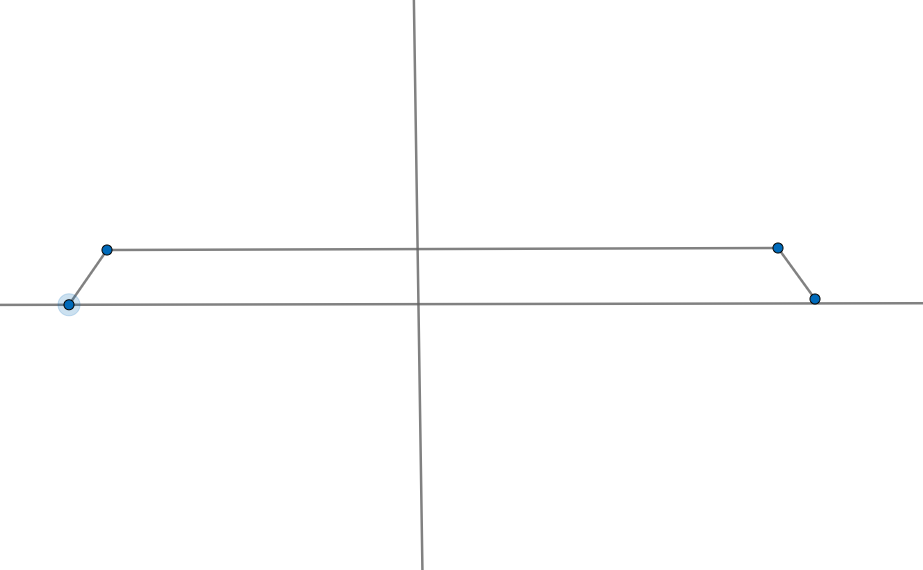
\includegraphics[width=2.5in]{spectralcluster/images/cheeger-counterexample.png}
\caption{
  The function $\rho_1$, a $1$-Lipschitz counterexample to Cheeger's inequality
  when $\alpha + \gamma > 2\beta$. 
  The height of the
  function is $\epsilon/2$, and the length of the supporting
  interval is roughly $\frac{2}{\epsilon}$.
 }
\label{fig:buser-counterexample}
\end{figure}

\begin{figure}[H]
\centering
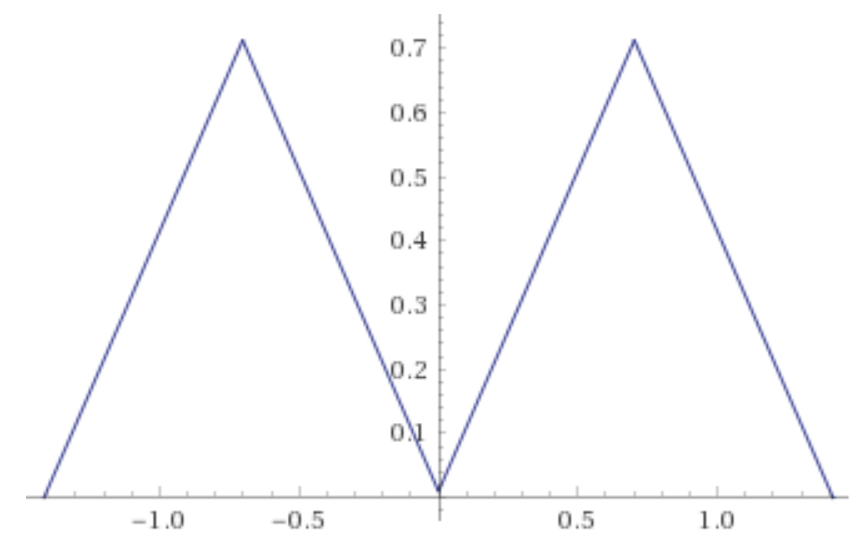
\includegraphics[width=2.5in]{spectralcluster/images/buser-counterexample.png}
\caption{
  The function $\rho_2$, a $1$-Lispchitz counterexample to Buser's inequality
  when $\gamma \geq 1$ and $ \gamma - 1 < \beta$.
 }
\label{fig:buser-counterexample}
\end{figure}


We will show that if $\alpha, \beta, \gamma$ satisfy $\alpha +
\gamma > 2\beta$, then the Cheeger inequality will fail for
$\rho_1$, and if $\gamma \geq 1$ and $\gamma - 1 < \beta$, then the Buser inequality
will fail for $\rho_2$.

In example $\rho_1$, let $\epsilon < 0.01$. The $(\alpha, \beta)$ isoperimetric constant
$\Phi$ is $O((1/\epsilon)^{\alpha - \beta - 1})$, and the eigenvalue
is $O((1/\epsilon)^{\alpha - \gamma - 2})$.  Therefore, the Cheeger
inequality will fail for some $\epsilon$ if $2 (\alpha - \beta - 1) > \alpha - \gamma -
2$, or $\alpha + \gamma > 2\beta$. This proves
Lemma~\ref{lem:cheeger-converse}.

In example $\rho_2$, let $\epsilon < 0.01$. The $(\alpha, \beta)$ isoperimetric constant
$\Phi$ is $O(\epsilon^{\beta})$. The eigenvalue
$\lambda_2$ is lower bounded by $O(\epsilon^{\gamma-1})$ when
$\gamma > 1$, and $\ln(1/\epsilon)$ when $\gamma =1$.
In either case, the Buser inequality will fail if $\gamma - 1 <
\beta$, proving Lemma~\ref{lem:buser-converse}.

We show details of our eigenvalue and isoperimetry calculations
in Appendix~\ref{app:examples}.


%!TEX root = ms.tex

\section{Buser Inequality for Probability Density Functions} \label{sec:buser}

In this section the theory of functions of bounded variation is used to
justify certain formal calculations. The key step is to define the geometric
quantities variationally.

\begin{definition}
  For a measurable set $A\subseteq \Re^d$ and $\rho:\Re^d \rightarrow
  \Re_{\geq 0}$ integrable define
  \begin{align*}
    \abs{A}_\alpha \coloneqq \int_A \rho^\alpha(x)\,dx.
  \end{align*}
\end{definition}

We define the weighted boundary area
variationally~\cite{betta2008weighted,parini2011introduction}.

\begin{definition}
\label{def:betaBdy}
For $\rho:\Re^d \rightarrow \Re_{\geq 0}$ integrable and $A\subseteq\Re^d$
the weighted perimeter of $A$ is
\begin{align*}
\abs{\boundary A}_\beta \coloneqq \sup\set{
\int_A \div(\rho^\beta (x) \phi(x))\,dx
\smid \phi\in C_c^1(\Re^d),\, \norm{\phi}_{\infty}\leq 1}.
\end{align*}
\end{definition}

\begin{remark}
  This definition corresponds to the intuitive definition of the
  boundary integral of $\rho^\beta$ when $\boundary A$ is sufficiently
  regular.  Specifically, if $A\subseteq\Re^d$ has smooth boundary
  and then,
  $$
  \abs{\boundary A}_\beta = \int_{\boundary A} \rho^\beta(x)\,d \mc H^{n-1}(x),
  $$
  where $\mc H^{n-1}$ denotes surface (Hausdorff) measure.
\end{remark}

\begin{definition}
  Let $A\subseteq\Re^d$ be a set of finite perimeter such that
  $\abs{A}_\alpha,\abs{\Re^d\setminus A}_\alpha >0$. The
  \textit{isoperimetric ratio} of the cut induced by $A$ is
\begin{align*}
\Phi(A) &\coloneqq \frac{\abs{\boundary A}_\beta}
{\min\left(\abs{A}_\alpha,\abs{\Re^d\setminus A}_\alpha\right)}
\end{align*}
and the \textit{isoperimetric constant} with weight $\rho$ is
\begin{align*}
  \Phi \coloneqq \inf_{A\subseteq \Re^d} \Phi(A).
\end{align*}
Here, $A$ is taken over sets of finite perimeter such that
$\abs{A}_\alpha,\abs{\Re^d \setminus A}_\alpha>0$.
\end{definition}

\subsection{Weighted Buser-type Inequality}

We now prove our weighted Buser-type inequality
Theorem~\ref{thm:Cheeger-Buser}. We state our result in terms of
general $(\alpha, \beta, \gamma)$.

\begin{theorem}
  \label{thm:buser_n}
  Let $\rho: \Re^d \to \Re_{\geq 0}$ be an $L$-Lipschitz function,
  $\lambda_2$ be a $(\alpha, \gamma)$-principal eigenvalue, and
  $\Phi$ the $(\alpha, \beta)$ isoperimetric cut.

  Then:
  \begin{align*}
    \lambda_2 \leq 3 \cdot 2^{\beta + 1} d \linf{\rho^{\gamma-\beta-1}}
    \max\left(L \Phi, 2^{\beta+1}\linf{\rho^{\alpha+1-\beta}} \Phi^2 \vph\right)
\end{align*}
\end{theorem}

We note that when setting $(\alpha, \beta, \gamma) = (1,2,3)$,
the above expression simplifies into:

\begin{align*}
  \lambda_2 \leq 24 d 
  \max\left(L \Phi, 8 \Phi^2 \vph\right).
\end{align*}

\subsection{Proof Strategy: Mollification by Disks of Radius
  Proportional to \texorpdfstring{$\rho$}{rho}}
To prove Theorem \ref{thm:buser_n}, for $A \subset \Re^d$ fixed, we
construct an approximation $u_\theta$ of the characteristic function,
$u$, of $A$ for which the numerator and denominator of the Rayleigh
quotient, $R(u_\theta)$, approximate respectively the numerator and
denominator of this expression.  Specifically, $u_\theta$ will
constructed as a mollification of $u$, Recall the following two
equivalent definitions of a mollification.  They are equivalent by the
change of variables $z = x-\theta \rho(x) y$.

\begin{equation} \label{eqn:utheta}
u_\theta(x) 
\coloneqq \int_{B(0,1)} \!\!\! u(x-\theta \rho(x) y) \phi(y) \, dy
= \int \! u(z) \phi_{\theta \rho(x)}(x-z) \, dz,
\quad \text{ where } \quad
\phi_{\eta}(z) 
= \frac{1}{\eta^d} \phi\left(\frac{z}{\eta}\right),
\end{equation}

with $\theta > 0$ a parameter to be chosen and $\phi:\Re^d \rightarrow
[0,\infty)$ a smooth radially symmetric function supported in the unit
open ball $B(0,1)=\{x \in \Re^d \;| \; |x| < 1\}$ with unit mass
$\int_{\Re^d} \phi = 1$. When $\rho$ is constant it follows from the
Tonelli theorem that $\lone{u_\theta} = \lone{u}$; when $\rho$ is not
constant the following lemma shows that the latter still bounds the
former.


\subsection{Key Technical Lemma: Bounding $L_1$ norm of a
  function with the $L_1$ norm of its
    mollification}\label{sec:key_lemma}
The following is our primary technical lemma, which roughly bounds the
$L_1$ norm of a mollified function $f$ by the $L_1$
norm of the original $f$. Here, the mollification radius is
determined by a function $\delta(x)$.
\begin{lemma} \label{lem:lonetheta} 

  Let
  $\delta:\RR^d\to\RR$ be Lipschitz continuous with Lipschitz constant
  $|\grad\delta(x)| \leq c < 1$ for almost every $x \in \bbR^d$. Let
  $\phi:\RR^d\to\RR_{\geq 0}$ be smooth, $\int_{\RR^d}\phi = 1$, and
  $\supp(\phi)\subseteq B(0,1)$.  Then
  \[
  \frac{1}{1+c}\norm{f}_{L^1}
  \leq \int_{\RR^d} \int_{B(0,1)} 
  \abs{f(x-\delta(x) y)}\phi(y)\,dy\,dx\leq
  \frac{1}{1-c}\norm{f}_{L^1},
  \qquad
  f \in L^1(\RR^d).
  \]
\end{lemma}

\begin{proof} (of Lemma~\ref{lem:lonetheta})
An application of Tonelli's theorem shows
\begin{align}
\int_{\RR^d} \int_{B(0,1)} \abs{f(x-\delta(x) y)}\phi(y)\,dy\,dx
=  \int_{B(0,1)}\phi(y)\int_{\RR^d} \abs{f(x-\delta(x)y)}\,dx\,dy.
\end{align}
Fix $y\in B(0,1)$ and consider the change of variables $z = x-\delta(x)y$. The
Jacobian of this mapping is $I - y \otimes \nabla \delta(x)$ which by Sylvester's determinant theorem has
determinant $1-y.\nabla \delta(x) > 0$. It follows that
\begin{align}
\int_{\RR^d} \int_{B(0,1)} 
\abs{f(x-\delta(x) y)}\phi(y)\,dy\,dx
=  \int_{B(0,1)}\phi(y)\int_{\RR^d} 
\frac{|f(z)|}{1-y.\nabla \delta(x)} \, dx \,dy,
\end{align}
and the lemma follows since $1-c \leq 1-y.\nabla \delta(x) \leq 1+c$.
\end{proof}
(Here, $a.b$ denotes the dot product between $a$ and $b$.)

We present the following simple corollaries, which is the primary
way our proof makes use of Lemma~\ref{lem:lonetheta}

\begin{corollary}\label{cor:lonetheta}
For any Lipschitz continuous function $\rho: \bbR^d \rightarrow \bbR^{\geq 0}$
with Lipschitz constant $L$ and any $\theta$ with $0 < \theta L < 1$, we have:
$$
\frac{1}{1+\theta L} \lone{\rho^\beta\nabla u}
\leq \int_{\bbR^d} \int_{B(0,1)} \rho^\beta ( x - \theta \rho(x) y)
  |\nabla u(x-\theta \rho(x)y)| \phi(y)\,dy\,dx
 \leq \frac{1}{1-\theta L} \lone{ \rho^\beta\nabla u},
$$
when $\rho^\beta |\nabla u| \in \Lone$.
\end{corollary}

\begin{proof} (of Corollary~\ref{cor:lonetheta}) Apply
  Lemma~\ref{lem:lonetheta} with $\delta(x) = \theta \rho(x)$, and
  $f(x) = \rho^\beta(x) \nabla u(x)$.
\end{proof}

This corollary will be used to bound the numerator of our
Rayleigh quotient.
Note that the expression
\[ \int_{\bbR^d} \int_{B(0,1)} \rho^\beta ( x - \theta \rho(x) y)
|\nabla u(x-\theta \rho(x)y)| \phi(y) dy dx
\]
is close to $\int_{\bbR^d} \rho^\beta(x) \nabla |u_\theta(x)| dx$ when
$\theta \leq \frac{1}{2L}$. This is the guiding intuition behind how
Corollary~\ref{cor:lonetheta} and Lemma~\ref{lem:lonetheta} will be
used, and will be formalized later in our proof of
Theorem~\ref{thm:buser_n}.

We present another simple corollary whose proof is equally
straightforward. This corollary will be used to bound the denominator,
and is a small generalization of Corollary~\ref{cor:lonetheta}. We
write down both corollaries anyhow, since this will make it easier to
interpret our bounds on the Rayleigh quotient.

\begin{corollary}\label{cor:lone-t-theta}
For any Lipschitz continuous function $\rho: \bbR^d \rightarrow \bbR^{\geq 0}$
with Lipschitz constant $L$, any $0 < t < 1$, and any $\theta$ with $0 < \theta L < 1$, we have:
$$
\frac{1}{1+\theta L} \lone{\rho^\beta \nabla u}
\leq \int_{\bbR^d} \int_{B(0,1)} \rho^\beta ( x - \theta t \rho(x) y)
|\nabla u(x-\theta t \rho(x)y)| \phi(y)\,dy\,dx
\leq \frac{1}{1-\theta L} \lone{ \rho^\beta \nabla u}
$$
\end{corollary}

\begin{proof} (of Corollary~\ref{cor:lone-t-theta})
    Apply Lemma~\ref{lem:lonetheta} with
    $\delta(x) = \theta t \rho(x)$, and $f(x) = \rho^\beta(x) \nabla u(x)$.
\end{proof}

A key technical step is to observe that the above two corollaries hold
when $u$ is a function of bounded variation provided the left and right
terms are interpreted as their variation. In particular, consider $A
\subset \Re^d$ with finite perimeter and let $u$ be the
characteristic function of $A$. ($u(x) = 1$ if $x \in A$ and zero
otherwise). Then there exists a sequence of functions
$\{u_n\}_{n=1}^\infty \subset C^\infty(\Re^d)$ with $u_n \rightarrow
u$ in $\Lone$ for which \cite{EvansMeasure15}
\begin{equation} \label{eqn:Aapprox}
\abs{\boundary A}_\beta
= \lim_{n \rightarrow \infty} \int_\Omega  \rho^\beta|\nabla u_n|
\eqqcolon  \int_\Omega  \rho^\beta|\nabla u|.
\end{equation}
Interchanging $A$ and $\Omega \setminus A$ if necessary, it follows that
$\Phi(A)$ defined in Definition \ref{def:betaBdy} can be written as
$$
\Phi(A) 
= \frac{\int_\Omega \rho^\beta |\nabla u|}{\int_\Omega \rho^\alpha u}
= \lim_{n\to\infty}\frac{\int_\Omega \rho^\beta\abs{\grad u_n}}{\int_\Omega\rho^\alpha \abs{u_n}}.
$$

Now we are ready to prove our main Theorem, which is the Buser
inequality for probability densities stated in
Theorem~\ref{thm:buser_n}.
\begin{proof} (of Theorem \ref{thm:buser_n})

Fix $A \subset \RR^d$ with $|A|_\alpha \leq |1|_\alpha / 2$ and let
$u(x) = \chi_A(x)$ be the characteristic function of $A$. Setting 
$\ubar$ to be the weighted average of $u$,
\[
\ubar 
= \frac{\int \rho^\alpha u}{\int \rho^\alpha}
= \frac{\int_A \rho^\alpha}{\int \rho^\alpha}
= \frac{|A|_\alpha}{|1|_\alpha} \in [0,1/2],
\qquad \text{ then } \qquad
\int \rho^\alpha (u-\ubar) = 0,
\]
and
  \begin{equation}\label{eqn:blah}
\lone{\rho^\alpha(u-\ubar)} 
= \int \rho^\alpha |u-\ubar| = 2 |A|_\alpha (1-\ubar)
= 2 \int \rho^\alpha |u-\ubar|^2.
  \end{equation}

Since $|A|_\alpha = \lonea{u}$ and $1-\ubar \in [0,1/2]$ it follows that

\begin{equation} \label{eqn:PhiA}
  (1/2) \frac{\lone{\rho^\beta \nabla u}}{\lone{\rho^\alpha(u-\ubar)}} 
  \leq \Phi(A) = \frac{\lone{\rho^\beta \nabla u}}{\lone{\rho^\alpha u}}
  \leq \frac{\lone{\rho^\beta \nabla u}}{\lone{\rho^\alpha(u-\ubar)}}.
\end{equation}

In the calculations below we omit the limiting argument with smooth
approximations of $u$ in equation \eqnref{:Aapprox} which justify
formula involving $\nabla u$. In particular, only the $\Lone$ norm
of $\rho^\beta |\nabla u|$ will appear in the estimates since this
has meaning while the $\Ltwo$ norm is undefined.

Next, let $u_\theta$ be the mollification of (an extension of) $u$
given by equation \eqnref{:utheta}. Then $u_\theta(x)$ is a local
average average of $u$ so $u_\theta(x) \geq 0$, $\linf{u_\theta} \leq
1$ and $\linf{u-u_\theta} \leq 1$.  Letting $L$ denote the Lipschitz
constant of $\rho$, the parameter $\theta$ will to be chosen 
less than $1/(2L)$ so that that Lemma \ref{lem:lonetheta} is applicable
with constant $c = 1/2$.

The remainder of the proof constructs an upper bound on the numerator
  $\int_{\bbR^d} \rho^\gamma |\nabla u_\theta|^2$ of the Rayleigh quotient
for $u_\theta - \ubar_\theta$ by $\lone{\rho^\beta \nabla u}$ and to
  lower bound the denominator $\int_{\bbR^d} \rho^\alpha (u_\theta -
\ubar_\theta)^2$ by $\lone{\rho^\alpha (u-\ubar)}$. The conclusion
of the theorem then follows from equation \eqnref{:PhiA}.

\subsection{Upper Bounding the Numerator}
To bound the $L^2$ norm in
  the numerator of the Rayleigh quotient by the $L^1$ norm in the
  numerator of the expression for $\Phi(A)$ it is necessary to obtain
  uniform bound on $\rho(x) \nabla u_\theta(x)$. 
  
  \begin{lemma} \label{lem:rep1}
  Let $u$ be any function, and let $u_{\theta}$ be defined as in
  Equation~\ref{eqn:utheta}. Let $\rho: \Re^d \to \Re_{\geq 0}$ be an
  $L$-Lipschitz function.
  \begin{align}
  \linf{\rho (x) \nabla u_\theta(x)}
    \leq \linf{u} \frac{d(2+3L)}{\theta}
  \end{align}
  \end{lemma}

  \begin{proof}
  In order to prove this lemma, we first need to get a handle on
  $\nabla u_\theta(x)$, which is the gradient of $u$ after
  mollification by $\theta$.

  We take the
  the second representation of $u_\theta$ in equation \eqnref{:utheta}
  to get
  \begin{align}
  \nabla u_\theta(x) 
  = \int_{\bbR^d} u(z) \left\{
    \frac{-d}{\theta \rho(x)} \phi_{\theta \rho}(x-z) \nabla \rho
    + \frac{1}{(\theta \rho(x))^{d+1}} 
    \left( I 
      + \nabla \rho(x) \otimes \frac{x-z}{\theta \rho(x)} \right)
    \nabla \phi \left(\frac{x-z}{\theta \rho(x)} \right) \right\}
    \, dz,
  \end{align}
  which is a consequence of the multivariable chain rule. Here,
  $v \otimes u$ refers to the outer product of $v$ and $u$.

  Multiplying by $\rho$ gives:
  \begin{align}
  \rho (x) \nabla u_\theta(x) 
  = \int_{\bbR^d} u(z) \left\{
    \frac{-d}{\theta} \phi_{\theta \rho(x)}(x-z) \nabla
    \rho(x)
    + \frac{1}{(\theta^{d+1} \rho(x)^{d})} 
    \left( I 
      + \nabla \rho(x) \otimes \frac{x-z}{\theta \rho(x)} \right)
    \nabla \phi \left(\frac{x-z}{\theta \rho(x)} \right) \right\} \, dz.
  \end{align}
  Now, we can bound the above equation by carefully bounding each
  part. We note:
  \begin{align} \label{eq:Cphi-calculation}
    & \int_{\bbR^d} \frac{1}{(\theta^{d+1} \rho(x)^d)} \nabla
    \phi\left(\frac{x-z}{\theta \rho(x)} \right) dz
    \\
    & = \int_{\bbR^d} \frac{1}{(\theta^{d+1} \rho(x)^d)} \nabla
    \phi\left(\frac{-z}{\theta \rho(x)} \right) dz
    \\
     & = \frac{1}{\theta} \int_{\bbR^d} \nabla \phi(-y) dy
  \end{align}
  where the last step follows by a simple change of variable.
  Here, we note that $\nabla \phi(y)$ is a vector, and the
  integral is over $\bbR^d$, which is how we eliminated
  $\frac{1}{(\theta \rho(x))^d}$ from the expression.

  Next, we examine the term: 
  \begin{align}
    I + \nabla \rho(x) \otimes \frac{x-z}{\theta \rho(x)}
  \end{align}
  Here, we aim to bound the operator norm of this matrix. Here,
  we note that 
  \[ |x - z| \leq \theta \rho(x) \]
  when 
  \[
    \nabla \phi\left(\frac{x-z}{\theta \rho(x)}\right) \not= 0
  \]
  and thus, when the latter equation holds, we can say:

  \[
    \left| \frac{x-z}{\theta \rho(x)}\right| < 1.
  \]
  Since $|\nabla \rho(x) < L|$, we now have:
  \begin{align}\label{eqn:num-matrix-norm-bound}
    |I + \nabla \rho(x) \otimes \frac{x-z}{\theta \rho(x)}|_2 <
    3/2
  \end{align}
  Combining Equation~\ref{eqn:num-matrix-norm-bound} Equation~\ref{eq:Cphi-calculation} to show:
  \begin{align}
    & \left | \int_{\bbR^d}
    \frac{1}{(\theta^{d+1} \phi(x)^{d})} \left( I + \nabla \rho(x) \otimes \frac{x-z}{\theta \rho(x)}
    \right) \nabla \phi \left( \frac{x-z}{\theta \rho(x)}
    \right) dz \right| 
    \\
    & \leq \frac{(1 + L)}{\theta} \int_{\bbR^d} |\nabla\phi(y) | dy,
  \end{align}
  where $L = \linf{\nabla \rho}$ is the Lipschitz constant for $\rho$. 
  We note that Section~\ref{sec:dimension-dep} shows that 
  \begin{align}
    \int_{\bbR^d} | \nabla \phi(y) dy| \leq 2d.
  \end{align}
  and therefore:
  \begin{align}
    & \left | \int_{\bbR^d}
    \frac{1}{(\theta^{d+1} \phi(x)^{d})} \left( I + \nabla \rho(x) \otimes \frac{x-z}{\theta \rho(x)}
    \right) \nabla \phi \left( \frac{x-z}{\theta \rho(x)}
    \right) dz \right| 
    \\ \label{eq:rho-grad-utheta-2}
    & \leq \frac{2d(1+L)}{\theta}
  \end{align}

  Now we turn our attention to the first term, which is:
  \begin{align}
    \int_{\bbR^d} \frac{-d}{\theta} \phi_{\theta \rho(x)}(x-z)
    \nabla\rho(x) dz
  \end{align}
  We note that 
  \[ 
    \int_{\bbR^d}\left| \phi_{\theta \rho(x)}(x-z)\right| dz
    = 1
  \]
  by our definition of $\phi$ (which was defined when we defined
      $u_\theta$). Combining this
  with $|\nabla \rho(x)| < L$, we get:
  \begin{align}
    & \int_{\bbR^d} \left | \frac{-d}{\theta} \phi_{\theta \rho(x)}(x-z)
    \nabla\rho(x) \right| dz
    \\ \label{eq:rho-grad-utheta-1}
    & < \frac{dL}{\theta}
  \end{align}
  Therefore, 
  \begin{align}
  &  \nonumber \left| \int_{\bbR^d} 
    \frac{-d}{\theta \rho(x)} \phi_{\theta \rho}(x-z) \nabla \rho
    + \frac{1}{(\theta \rho(x))^{d+1}} 
    \left( I 
      + \nabla \rho(x) \otimes \frac{x-z}{\theta \rho(x)} \right)
    \nabla \phi \left(\frac{x-z}{\theta \rho(x)} \right) \, dz
    \right|
    \\
    & \nonumber \leq \frac{d}{\theta}( L + 2(1+L)) 
    \\
  & = \frac{d(2+3L)}{\theta}.
  \label{eqn:}
  \end{align}
  where the first inequality comes from combining
  Equations~\ref{eq:rho-grad-utheta-2}
  and~\ref{eq:rho-grad-utheta-1}.

  This allows us to bound $\linf{\rho(x) \nabla u_{\theta}(x)}$:
  \begin{align}
  & \linf{\rho (x) \nabla u_\theta(x)}
  \\
  & = \linf{ \left| \int_{\bbR^d} u(z) \left\{
    \frac{-d}{\theta} \phi_{\theta \rho(x)}(x-z) \nabla
    \rho(x)
    + \frac{1}{(\theta^{d+1} \rho(x)^{d})} 
    \left( I 
      + \nabla \rho(x) \otimes \frac{x-z}{\theta \rho(x)} \right)
    \nabla \phi \left(\frac{x-z}{\theta \rho(x)} \right) \right\}
  \, dz \right| }
  \\
  & \leq \linf{u} \linf{ \int_{\bbR^d} \left| 
    \frac{-d}{\theta} \phi_{\theta \rho(x)}(x-z) \nabla
    \rho(x)
    + \frac{1}{(\theta^{d+1} \rho(x)^{d})} 
    \left( I 
      + \nabla \rho(x) \otimes \frac{x-z}{\theta \rho(x)} \right)
    \nabla \phi \left(\frac{x-z}{\theta \rho(x)} \right)
  \right| \, dz}
  \\
  & \leq \linf{u} \frac{d(2+3L)}{\theta}
  \end{align}
  where we make use of the fact that
    $\linf{ab} < \linf{a}\lone{b}.$
  This completes our proof.
  \end{proof}

  Next, we want an $L_1$ bound on $\rho^{\beta}(x) \nabla
  u_{\theta}(x)$.

  \begin{lemma} \label{lem:rep2}
  Let $u$ be any function, and let $u_{\theta}$ be defined as in
  Equation~\ref{eqn:utheta}. Let $\rho:\Re^d \to \Re_{\geq 0}$ be an
  $L$-Lipschitz function, and
  let $\theta L < 1/2$.

  Then:
  \begin{align}
      \lone{\rho^\beta(x) \nabla u_{\theta}(x)} \leq C_{\beta}
      \lone{\rho^\beta(x) \nabla u(x)}
  \end{align}
  \end{lemma}
  \begin{proof}
  First, we take the gradient 
  first representation of $u_\theta$
  in equation \eqnref{:utheta}. Using the chain rule gives us an
  alternate form for $\nabla u_\theta(x)$:

  \begin{align}
  \nabla u_\theta(x) 
  = \int_{\Re^d} 
  (I - \theta \nabla \rho \otimes y) \nabla u(x-\theta \rho y) \phi(y) \, dy,
  \end{align}
  so
  \begin{align}\label{eqn:rhoNablaUtheta}
  \rho^\beta(x) \nabla u_\theta(x) 
  = \int_{\Re^d} 
  (I - \theta \nabla \rho \otimes y)
  \frac{\rho^\beta(x)}{\rho^\beta(x-\theta \rho y)}
  \rho^\beta(x-\theta \rho y) \nabla u(x-\theta \rho y) \phi(y) \, dy.
  \end{align}

  The ratio in the integrand is bounded using the Lipschitz assumption
  on $\rho$ (and $|y| \leq 1$),
  \begin{equation} \label{eqn:rhoRatio}
    \frac{\rho(x)}{\rho(x-\theta \rho y)}
    \leq \frac{\rho(x)}{\rho(x) - L \theta \rho(x)}
    = \frac{1}{1 - L \theta} \leq 2,
    \qquad \text{ when } \theta < 1 / (2L).
  \end{equation}
  Note that 
  \begin{align} \label{eqn:matrix-norm} 
  \left\| I - \theta \nabla \rho \otimes y \right\|_2 \leq 3/2
  \end{align}
  where $\|M\|_2$ represents the $\ell^2$ matrix norm of $M$. This is
  because $|\nabla \rho(x) | \leq L$, and
  $\theta L < 1/2$, and $|y| \leq
  1$ every time $\phi(y) \not= 0$, and thus 
  \[ 
   \frac{I}{2} \preceq  I - \theta \nabla \rho \otimes y
   \preceq \frac{3I}{2}.
    \]
  
 Therefore, we can now apply Corollary~\ref{cor:lonetheta}
 to Equation~\eqnref{:rhoNablaUtheta} to show:
  \begin{align}
  \nonumber 
  & \lone{\rho^\beta(x) \nabla u_\theta(x)} 
  \\  \nonumber
  & \leq \|I - \theta \nabla \rho(x) \otimes y\|_2
  \cdot \max_x\left(\frac{\rho(x)}{\rho(x - \theta \rho
        y)}\right) \cdot
  \int_{\bbR^d} \left| \int_{\bbR^d} \rho^{\beta}(x - \theta \rho y) \nabla u(x - \theta \rho y)
    \phi(y) dy \right|
  \\ \nonumber 
  & \leq 3 \cdot 2^{\beta - 1} \int_{\bbR^d} \rho^\beta(x -
      \theta \rho(x) y) \nabla u (x - \theta \rho (x) y 
  \\ \nonumber
  & 
  \leq 3 \cdot 2^\beta \lone{\rho^\beta \nabla u},
  \qquad \text{ when } \theta < 1 / (2L).
  \end{align}
  here, the first inequality comes from the equation $\lone{abc}
  \leq \linf{a}\linf{b}\lone{c}$, the second inequality comes
  from Equations~\ref{eqn:rhoRatio} and~\ref{eqn:matrix-norm}, and the
  third inequality comes
  from Corollary~\ref{cor:lonetheta} assuming $\theta L \leq
  1/2$. 
  \end{proof}

  \begin{lemma}\label{lem:num}
  For any $L$-Lipschitz distribution $\rho$, any function $u$, and any $\theta$ such that $\theta L <
  1/2$:

  \begin{align}
  \int_{\bbR^d} \rho^\gamma |\nabla u_\theta|^2
  \leq  C_\beta \linf{\rho^{\gamma-\beta-1}} \frac{d(2+3L)}{\theta} 
  \linf{u} \lone{\rho^\beta \nabla u},
  \end{align}
  \end{lemma}

  \begin{proof}
  Combining the two estimates from Lemma~\ref{lem:rep1}
  and~\ref{lem:rep2} gives an upper bound for the Rayleigh
  quotient 
  \begin{align}
  \int_{\bbR^d} \rho^\gamma |\nabla u_\theta|^2
  = \int_{\bbR^d} \rho^{\gamma-\beta-1} \,
  \rho |\nabla u_\theta| \, \rho^\beta |\nabla u_\theta|
  \leq 3 \cdot 2^{\beta + 1} \linf{\rho^{\gamma-\beta-1}} \frac{d(2+3L)}{\theta} 
  \linf{u} \lone{\rho^\beta \nabla u},
  \end{align}
  \end{proof}

  We note that in the case where $\gamma = \beta + 1$, and if $u$ is a step
  function, the expression would
  simplify to:
  \[ \int_{\bbR^d}
  |\rho^{\gamma} |\nabla u_\theta|^2
  \leq 3 \cdot 2^{\beta + 1} \frac{d(2+3L)}{\theta} 
  \linf{u} \lone{\rho^\beta \nabla u},
  \]

\subsection{Lower Bound on the Denominator}
Let $\ubar$ and
  $\ubar_\theta$ be the $\rho^\alpha$--weighted averages of $u$ and
  $u_\theta$. For any function $f$, let $\ltwoa{f}$ denote the $L^2$ norm of $\rho^\alpha
  f$, and let $\lone{f}$ denote the $L^1$ norm of $\rho^\alpha f$ for
  functions $f$ where these two quantities are well defined.
  Our core lemma is a bound on $\ltwoa{u_\theta-\ubar_\theta}$ in
  terms of $l_1$ and weighted $l_1$ norms of $\nabla u$ and $u -
  \ubar$ respectively.
  \begin{lemma}\label{lem:denom}
  Let $\rho$ be an $L$-Lipschitz function $\rho: \Re^d \to
  \Re_{\geq 0}$, and let $\theta$ be such
  that $\theta L < 1/2$.
  Let $u$ be an indicator function of a set $A$ with finite
  $\beta$-perimeter. Let $\ubar$ be defined as $\ubar(x):=u(x) - \int u(y) dy$
    $u_\theta$ be defined as in Equation~\ref{eqn:utheta}, and
    $\ubar_\theta$ be defined as $\ubar_\theta(x) := u_\theta(x)
    - \int
    u_\theta(y) dy$.
    Then:
  \begin{align}
  \ltwoa{u_\theta - \ubar_\theta}^2
  \geq (1/4) \lonea{u-\ubar} 
  - C(\beta) \theta \linf{\rho^{\alpha+1-\beta}} \lone{\rho^\beta \nabla u},
  \qquad \text{ when } \theta < 1 / (2L).
  \end{align}
  \end{lemma}

  Note that when $\alpha + 1 = \beta$, as is true when $(\alpha,
      \beta, \gamma) = (1,2,3)$, the inequality in
  Lemma~\ref{lem:denom} becomes:

  \[
  \ltwoa{u_\theta - \ubar_\theta}^2
  \geq (1/4) \lonea{u-\ubar} 
  - C(\beta) \theta \lone{\rho^\beta \nabla u},
  \qquad \text{ when } \theta < 1 / (2L).
  \]
  The estimate in Lemma~\ref{lem:denom} will be combined with the
  estimate in Lemma~\ref{lem:num} to prove
  Theorem~\ref{thm:buser_n}
  in Section~\ref{sec:rayleigh-bound}.


  \begin{proof} The key to this proof is to upper bound the
  quantity $\ltwoa{u_\theta - \ubar_\theta}$ with the expression
  appearing in Corollary~\ref{cor:lone-t-theta}. We will do so by
  a series of inequalities, application of the fundamental
  theorem of calculus, and more.

  Using the property that subtracting the average from a
  function reduces the $L^2$ norm it follows that
  \begin{align}
  \nonumber
  & \ltwoa{u_\theta - \ubar_\theta}
  \\
    \nonumber
  & \geq \ltwoa{u-\ubar} - \ltwoa{u_\theta - u - (\ubar_\theta-\ubar)}
  \\
    \nonumber
  &\geq \ltwoa{u-\ubar} - \ltwoa{u_\theta - u}.
  \end{align}
  If $a \geq b-c$ then $a^2 \geq b^2/2 - c^2$, so a lower bound for
  the denominator of the Rayleigh quotient
  \begin{align} \label{eqn:utmu}
    & \ltwoa{u_\theta - \ubar_\theta}^2
    \\
    \nonumber
    &\geq (1/2) \ltwoa{u-\ubar}^2 - \ltwoa{u_\theta - u}^2
    \\
    \nonumber
    & \geq (1/4) \lonea{u-\ubar} - \lonea{u_\theta - u},
  \end{align}
  where the identity $\ltwoa{u-\ubar}^2 = \lonea{u-\ubar}/2$ from
  Equation~\ref{eqn:blah}, and the bound
  $\linf{u_\theta - u} \leq 1$, were used in the last step.

  It remains to estimate the difference $\lonea{u_\theta - u}$. To
  do this, we use the multivariable fundamental
  theorem of calculus to write
  \begin{eqnarray*}
    u_\theta(x) - u(x)
    &=& \int (u(x - \theta \rho y) - u(x)) \phi(y) \, dy \\
    &=& \int \! \int_0^1
    -\theta \rho(x) \nabla u(x - t \theta \rho(x) y).y \phi(y) \, dt \, dy \\
    &=& \int \! \int_0^1
    \frac{-\theta \rho(x)}{\rho^\beta(x-t\theta \rho(x) y)} 
    \rho^\beta(x - t\theta \rho(x) y) \nabla u(x - t \theta
        \rho(x) y).y \phi(y) \, dt \, dy,
  \end{eqnarray*}
  where the first and second equalities came from application of
  the multivariable fundamental theorem of calculus, and the last
  equation is straightforward. This tells us that:
  \begin{align}
  \notag
  & \rho^{\alpha}(x) ( u_\theta \rho(x) - u(x) )
  \\
  \notag
  & = \int \! \int_0^1
  \frac{-\theta \rho^{\alpha+1}(x)}{\rho^\beta(x-t\theta \rho y)} 
  \rho^\beta(x - t\theta \rho(x) y) 
  \nabla u(x - t \theta \rho(x) y).y \phi(y) \, dt \, dy.
  \\
    \label{eqn:utheta-l1-alpha}
  &= \int \! \int_0^1
  \frac{\rho^\beta(x)}{\rho^\beta (x- t \theta \rho(x)y)}
  \frac{-\theta \rho^{\alpha+1}(x)}{\rho^\beta(x)}
  \rho^{\beta}(x - t \theta \rho(x) y )
  \nabla u(x - t \theta \rho(x) y).y \phi(y) \, dt \, dy.
  \end{align}
  Equation \eqnref{:rhoRatio} bounds the ratio $\rho(x)/ \rho(x -
    t\theta \rho(x) y)$ as less than $2$ when $\theta L < 1/2$,
  so Equation~\eqnref{:utheta-l1-alpha} is always less than or
  equal to:
  \begin{align}
  \int \! \int_0^1
  2^{\beta}
  \frac{-\theta \rho^{\alpha+1}(x)}{\rho^\beta(x)}
  \rho^{\beta}(x - t \theta \rho(x) y )
  \nabla u(x - t \theta \rho(x) y).y \phi(y) \, dy \, dt.
  \end{align}

  An application of Corollary \ref{cor:lone-t-theta} then shows
  \begin{align}
  & \int \! \int_0^1
  2^{\beta}
  \frac{-\theta \rho^{\alpha+1}(x)}{\rho^\beta(x)}
  \rho^{\beta}(x - t \theta \rho(x) y )
  \nabla u(x - t \theta \rho(x) y).y \phi(y) \, dy \, dt.
  \\
  & \leq \int \! \int_0^1
  2^{\beta}
  \frac{-\theta \rho^{\alpha+1}(x)}{\rho^\beta(x)}
  \rho^{\beta}(x - t \theta \rho(x) y ) \ 
  \left|\nabla u(x - t \theta \rho(x) y) \phi(y)\right| \, dy \, dt.
  \\
  &
  \leq 2^{\beta+1} \linf{\rho^{\alpha+1-\beta}} \theta
  \int \! \int_0^1
  \rho^{\beta}(x - t \theta \rho(x) y ) \ 
  \left|\nabla u(x - t \theta \rho(x) y) \phi(y)\right| \, dy \, dt.
  \qquad \text{ when } \theta < 1 / (2L).
  \\
  &
  \leq 2^{\beta+1} \linf{\rho^{\alpha+1-\beta}} \theta \lone{\rho^\beta \nabla u}
  \end{align}
  where the last inequality follows from
  Corollary~\ref{cor:lone-t-theta}.

  Using this estimate in \eqnref{:utmu} gives a lower bound on the
  denominator of the Rayleigh quotient,
  \begin{align}
  \ltwoa{u_\theta - \ubar_\theta}^2
  \geq (1/4) \lonea{u-\ubar} 
  - 2^{\beta+1} \theta \linf{\rho^{\alpha+1-\beta}} \lone{\rho^\beta \nabla u},
  \qquad \text{ when } \theta < 1 / (2L).
  \end{align}
  as desired.
  \end{proof}

  \subsection{Bounding the Rayleigh
    Quotient (Proof of Theorem~\ref{thm:buser_n})}\label{sec:rayleigh-bound}
  Combining Lemmas~\ref{lem:num} and Lemmas~\ref{lem:denom}
  provides an upper bound for the Rayleigh quotient of $u_\theta - \ubar_\theta$,
  \begin{eqnarray*}
    \lambda_2 
    &\leq& \frac{\int_{\bbR^d} \rho^\gamma |\nabla u_\theta|^2}
    {\int_{\bbR^d} \rho^\alpha (u_\theta - \ubar_\theta)^2} \\
    &\leq&  \frac{d \cdot 3 \cdot 2^{\beta}}{\theta}
    \frac{\linf{\rho^{\gamma-\beta-1}} (2+3L) \lone{\rho^\beta \nabla u}}
    {\lonea{u-\ubar} 
      - 2^{\beta+1} \theta \linf{\rho^{\alpha+1-\beta}} \lone{\rho^\beta \nabla u}} \\
    &\leq&  \frac{d \cdot 3 \cdot 2^{\beta}}{\theta}
    \frac{\linf{\rho^{\gamma-\beta-1}} (2+3L)}
    {1 - 2^{\beta + 1} \theta \linf{\rho^{\alpha+1-\beta}} \Phi(A)} \Phi(A).
  \end{eqnarray*}
  Selecting $\theta = (1/2)
  \min\left(1/\left(2^{\beta+1}\linf{\rho^{\alpha+1-\beta}}
        \Phi(A)\right), 1/L
  \right)$ shows
  \[
  \lambda_2 \leq 2 d \cdot 3 \cdot 2^{\beta}
\linf{\rho^{\gamma-\beta-1}}(2+3L) 
  \max\left(L \Phi(A), 2^{\beta+1}\linf{\rho^{\alpha+1-\beta}} \Phi(A)^2 \vph\right).
  \]
  When $\gamma = (1,2,3)$, this simplifies into:
  \[
  \lambda_2 \leq 12(2+3L) d
  \max\left(L \Phi(A), 8 \Phi(A)^2 \vph\right).
  \]
  We note that, via the work shown in
  Section~\ref{sec:scaling},  we can strengthen our inequality
  to:
  \[
  \lambda_2 \leq 24 d
  \max\left(L \Phi(A), 8 \Phi(A)^2 \vph\right).
  \]

  \qedhere


\subsection{Gradient of Mollifier}\label{sec:dimension-dep}
Let $\phi$ be a standard mollifier i.e. $\phi\in C_c^\infty(\RR^d)$
is a function from $\RR^d\to [0,\infty)$ satisfying $\int_{\RR^d}
  \phi\,dx = 1$ and $\supp(\phi)\subseteq B(0,1)$.  We will define
  $\phi$ by its profile. Namely, let $\phihat(r):[0,\infty)
    \rightarrow [0,1]$ be a fixed monotone decreasing profile with
    $\phihat(0)=1$, $0 < \phihat(r) < 1$ for $0 < r < 1$, and
    $\phihat(r) = 0$ for $r \geq 1$. Then define $\phi:\Re^d
    \rightarrow \Re$ by $\phi(x) = c \phihat(|x|)$ with $c > 0$ chosen
    so that $\int_{\Re^d} \phi(x) \, dx = 1$; that is,

\[
1 = \int_{\Re^d} \phi(x) \, dx
= c |S^{d-1}| \int_0^1 \phihat(r) r^{d-1} \, dr
\qquad \Rightarrow \qquad
c = \frac{1}{|S^{d-1}| \int_0^1 \phihat(r) r^{d-1} \, dr},
\]

where $|S^{d-1}|$ is the $(d-1)$--area of the unit sphere in $\Re^d$.
We claim the $L_1$ norm of the gradient of $\nabla \phi(x)$ is linear in $d$.
\begin{lemma}\label{lem:molli}
  \[
  \int_{\Re^d} |\nabla \phi(x)| \, dx   
\leq (d-1) \left( \frac{d 2^d}{\phihat(1/2)} \right)^{1/(d-1)}
\stackrel{d \rightarrow \infty}{\longrightarrow} 2(d-1).
\]
For the classic mollifier $\phihat(r)=\exp(-1/(1-r^2))$ we get
  \[
  \int_{\Re^d} |\nabla \phi(x)| \, dx  \leq 2d.
\]
\end{lemma}

From the formula $\nabla \phi(x) = c \phihat'(|x|) (x/|x|)$ we compute
\begin{eqnarray*}
\int_{\Re^d} |\nabla \phi(x)| \, dx
&=& c |S^{d-1}| \int_0^1 |\phihat'(r)| r^{d-1} \, dr \\
&=& c |S^{d-1}| \int_0^1 -\phihat'(r) r^{d-1} \, dr \\
&=& c |S^{d-1}| \int_0^1 \phihat(r) (d-1) r^{d-2} \, dr \\
&=& (d-1) \frac{\int_0^1 \phihat(r) r^{d-2} \, dr}
{\int_0^1 \phihat(r) r^{d-1} \, dr}.
\end{eqnarray*}
To estimate the numerator use Holder's inequality: for
$1 \leq s, s' \leq \infty$ with $1/s + 1/s' = 1$ 
$$
\int f g 
\leq \left(\int |f|^s \right)^{1/s} \left(\int |g|^{s'} \right)^{1/s'}.
$$
Set $s = (d-1)/(d-2)$ and $s' = d-1$ to get
$$
\int_0^1 \phihat(r) r^{d-2} \, dr
= \int_0^1 \phihat(r)^{1/s} r^{d-2} \times \phihat(r)^{1/s'}  \, dr
\leq \left(\int_0^1 \phihat(r) r^{d-1} \, dr \right)^{1/s}
\left(\int_0^1 \phihat(r) \, dr \right)^{1/s'}.
$$
It follows that
\begin{equation}\label{eq:molli0}
\int_{\Re^d} |\nabla \phi(x)| \, dx
\leq (d-1) \left( \frac{\int_0^1 \phihat(r) \, dr}
{\int_0^1 \phihat(r) r^{d-1} \, dr} \right)^{1/(d-1)}.
\end{equation}
Since $0 \leq \phihat(r) \leq 1$ we can bound the numerator
by $1$, and since $\phihat(r)$ is monotone decreasing we have
$\phihat(r) \geq \phihat(1/2)$ on $(0,1/2)$, so 
\begin{equation}\label{eq:molli}
\int_{\Re^d} |\nabla \phi(x)| \, dx
\leq (d-1)
\left( \frac{1}{\phihat(1/2) \int_0^{1/2} r^{d-1} \, dr} \right)^{1/(d-1)} 
\leq (d-1) \left( \frac{d 2^d}{\phihat(1/2)} \right)^{1/(d-1)}
\stackrel{d \rightarrow \infty}{\longrightarrow} 2(d-1).
\end{equation}

It will be convenient to write equation~\ref{eq:molli} as a simple
inequality. Observer that
\[
 \left( \frac{d 2^d}{\phihat(1/2)} \right)^{1/(d-1)}
\]
is monotone decreasing. We now pick the classic
$\phihat(r) = \exp(-1/(1-r^2))$ we have $\phihat(1/2) \geq 1/4$ and if
$d \geq 5$ the right hand side of equation (\ref{eq:molli} is bounded
by $2d$. If $d < 5$ explicit computations of the integrals shows the
right hand side of equation (\ref{eq:molli0} is bounded by $2d$.







\end{proof}



\subsection{Scaling}\label{sec:scaling}

In this section we show that if one scales the density function $\rho$ then
the isoperimetric value $\Phi(A)$ and the Rayleigh quotient $R(u)$
scale nicely. More formally Let $A \subset \Omega \subseteq
\Re^d$, $\rho$ a density function over a domain $\Omega$, and
$u$ an arbitrary differentiable  function over $\Omega$.

Consider the transformation
$\xhat = \ell x$ with $\ell > 0$ which maps $\Omega$ to the domain
$\Omegahat = \{\ell x \sst x \in \Omega\}$. Given $u:\Omega \rightarrow
\Re$, we define $\uhat: \Omegahat \rightarrow \Re$ by $\uhat(\xhat) =
u(x)$. We will future scale $\rho$ by $\alpha \rhohat(\xhat) = \ell \, \rho(x)$ where
$\alpha > 0$.

\begin{theorem}\label{thm:scaling}
  When scaling by $\alpha$ and $\ell$ then
  \[   \Phi(A) = \alpha \Phihat(\Ahat) \] and
  \[  R(u)  = \alpha^2 \Rhat(\uhat) \quad \text{and thus} \quad\lambda_2 = \alpha^2 \hat{\lambda}_2\].
\end{theorem}

We will use this scaling theorem to improve the bounds
of theorem~\ref{thm:buser_n}. 

That is, if we have a density function $\rho$ over
a domain $\Omega$ the isoperimetric number that the fundamental eigenvalue only
change as a function  of the scaling.  Thus the optimal cut and eigenvector are
unchanged by scaling up to the transformation.

%% Given a domain $\Omega \subset \Re^d$, consider the transformation
%% $\xhat = \ell x$ with $\ell > 0$ which maps $\Omega$ to the domain
%% $\Omegahat = \{\ell x \sst x \in \Omega\}$. If $u:\Omega \rightarrow
%% \Re$, define $\uhat: \Omegahat \rightarrow \Re$ by $\uhat(\xhat) =
%% u(x)$.

If $u$ and $l$ are as defined above then we get the simple but basic identity. 
Suppose that $u: \R \rightarrow \R$ then: \[
\dbydp{u}{x} 
= \dbydp{\uhat}{\xhat} \dbydp{\xhat}{x}
= \dbydp{\uhat}{\xhat} \ell,
\qquad \text{ in general we get } \qquad
|\nabla u(x)| = \ell |\hat{\nabla} \uhat(\xhat)|.
\]

In the case of $\rho:\Omega \rightarrow (0,\infty)$, where
$\rhohat: \Omegahat \rightarrow (0,\infty)$ is defined by
$ \alpha \rhohat(\xhat) = \ell \, \rho(x)$ we get that
\[
|\nabla \rho(x)| = \alpha |\hat{\nabla} \rhohat(\xhat)|.
\]

It follows that $L_{\rhohat}$ and $L_\rho$, the Lipschitz constants
for $\rhohat$ and $\rho$,  satisfy $L_{\rhohat} = (1/\alpha) L_\rho$.

\begin{itemize}
\item
  Since $d\xhat = \ell^{d} \, dx$ we have
  \[
  \int_\Omega \rho \, dx = \frac{\alpha}{\ell^{d+1}} \int_{\Omegahat} \rhohat \, d\xhat, 
  \]
  %% so it is always possible to choose a scaling to get $\int_{\Omegahat}
  %% \rhohat = 1$.

\item
  If $A \subset \Omega$ and $\Ahat = \ell A \subset \Omegahat$,
  let $f_A(x) = 1$ if $x \in A$ and zero otherwise, and similarly
  $f_{\Ahat} = 1$ if $\xhat \in \Ahat$ and zero otherwise. We next perform
  a set of standard integral calculations.
  \begin{align}
  \int_\Omega \rho^2 |\nabla f_A| \, dx &=
  \int_{\Omegahat} (\frac{\alpha}{\ell})^2 \rhohat^2 \ell |\hat{\nabla} f_{\Ahat}|
  \, \frac{1}{\ell^d} d\xhat \label{eq:subsitution}\\
  &= \frac{\alpha^2}{\ell^{d+1}} \int_{\Omegahat} \rhohat^2  |\hat{\nabla} f_{\Ahat}|
  \, d\xhat \label{eq:integral1}
  \end{align}

  Equation~\ref{eq:subsitution} follows by making the substitutions:
  \[ \rho(x) = (\frac{\alpha}{\ell}) \rhohat(\xhat) \quad
  |\nabla f_A| = \ell |\hat{\nabla} f_{\Ahat}| \quad
  dx =  \frac{1}{\ell^d} d\xhat
  \]
  Observing the $f_A(x) = f_{\Ahat}(\xhat)$ we get the following identity.
\begin{equation}\label{eq:integral2}
 \int_\Omega \rho f_A \, dx
 = \int_{\Omegahat} \frac{\alpha}{\ell}  \rhohat f_{\Ahat} \frac{1}{\ell^d} \, d\xhat
   = \frac{\alpha}{\ell^{d+1}} \int_{\Omegahat} \rhohat f_{\uhat} \, d\xhat
\end{equation}

Combining equation~\ref{eq:integral1} and equation~\ref{eq:integral2}
we get that:

\begin{equation}
  \Phi(A) = \alpha \Phihat(\Ahat)
\end{equation}

\item
  We next do a similar calculation for the Rayleigh quotient.
  If $u:\Omega \rightarrow \Re$ and $\uhat(\xhat) = u(x)$, 
  the Rayleigh quotients can be computed as follows,
  \[
  \int_\Omega \rho^3 |\nabla u|^2 \, dx
  = \int_{\Omegahat} (\frac{\alpha}{\ell})^3 \rhohat^3
  \ell^2 |\hat{\nabla} \uhat|^2 \, \frac{1}{\ell^d} d\xhat
    = \frac{\alpha^3}{\ell^{d+1}} \int_{\Omegahat} \rhohat^3 |\hat{\nabla} \uhat|^2 \, d\xhat
 \]

\[
\int_\Omega \rho u^2 \, dx
= \int_{\Omegahat} \frac{\alpha}{\ell} \rhohat \uhat^2 \frac{1}{\ell^d} \, dx
= \frac{\alpha}{\ell^{d+1}} \int_{\Omegahat} \rhohat \uhat^2 \, dx
\]
Thus \[  R(u)  = \alpha^2 \Rhat(\uhat) \].
\end{itemize}

We next use our scaling result in the $(1,2,3)$ case
to our Buser-type bound, Theorem~\ref{thm:buser_n}.
Theorem~\ref{thm:buser_n} states that the following hold:

\begin{align}\label{eq:simple123}
  \lambda_2 \leq 24 d (1+L) 
  \max\left(L \Phi(A), 12 \Phi(A)^2 \vph\right).
\end{align}

We now make substitutions into equation~\ref{eq:simple123}
from Theorem~\ref{thm:scaling} and its proof for some parameter $\alpha$ to be determined.


\begin{align*}
  \lambda_2 = \alpha^2 \hat{\lambda}_2 &\leq  \alpha^2  24 d (1+\hat{L}) 
  \max\left(\hat{L} \Phihat(\Ahat), 12 \Phihat(\Ahat)^2 \vph\right) \\
  &=  \alpha^2  24 d (1+ (L/\alpha))
  \max\left((L/\alpha) (\Phi(A)/\alpha), 12 (\Phi(A)/\alpha)^2 \vph\right) \\
  &=  24 d (1+ (L/\alpha))
  \max\left(L \Phi(A), 12 \Phi(A)^2 \vph\right) \\
  &=  24 d \max\left(L \Phi(A), 12 \Phi(A)^2 \vph\right)
\end{align*}
where the last line holds when taking $\alpha$ to infinity.

Thus we get that $\lambda_2$ only depends linear in the dimension and  the Lipschitz constant:

\begin{corollary}\label{cor:strongBuser}
  \[
  \lambda_2 \leq  24 d \max\left(L \Phi, 12 \Phi^2 \vph\right)
  \]
\end{corollary}





\section{Cheeger Inequality for Probability Density Functions}\label{sec:cheeger}

In this section, we prove the Cheeger inequality from
Theorem~\ref{thm:Cheeger-Buser}. That is a weighted Cheeger inequality in higher dimensions.
This is the easier to prove than Buser's inequality, which
contrasts with what happens in the graph case (the graph Buser
    inequality is trivial).

For a simplified proof of the Cheeger inequality for distributions
in one-dimension, see Appendix~\ref{sec:one_dim}.

As we will see from simple counterexamples in
Section~\ref{sec:examples}, the Cheeger-direction does not
hold for all setting of $(\alpha,\beta,\gamma)$. The proof we give is
requires fewer assumptions than the Buser inequality for
probability densities. One, the Cheeger inequality is
independent of the Lipschitz constant of $\rho$ and two, the proof
also holds when $\rho$ is supported on a set
$\Omega \subset \mathbb{R}^d$.

The proof is almost identical to the proof in one dimension and only a
slight modification of standard proofs The only change in the proof is
replacing the change of variables formula with a co-area formula.  Let
$\rho:\Omega \to \RR_>$ be an Lipschitz density function that is
$(\alpha,\beta,\gamma)$-integrable over an open set $\Omega \subseteq
\RR^d$.  Note a stronger hypothesis  on $\Omega$ is that it is the support of
$\rho$ when  $\rho:\RR^d \to \RR_\leq$. 

\begin{theorem}
\label{thm:cheeger_n}
Let $\rho:{\Omega}\to\RR_{>0}$ be a Lipschitz function. Then,
\begin{align*}
\Phi^2 \leq 4 \norm{\rho^{\beta - \frac{\alpha+\gamma}{2}}}^2_\infty \lambda_2.
\end{align*}
In particular, when $(\alpha,\beta,\gamma) = (1,2,3)$ we have
\begin{align*}
\Phi^{2} \leq 4\lambda_2.
\end{align*}
\end{theorem}
Here, $\Phi$ is the optimal $(\alpha,\beta)$-sparsity of a cut
through $\rho$. We note that we can say something a little stronger:
\begin{theorem}
\label{thm:cheeger-sweep}
Let $\rho:{\Omega}\to\RR_{>0}$ be a Lipschitz function. 
Let $\Phi_{(\alpha,\beta,\gamma)}$ be the $(\alpha,\beta)$
sparsity of the $(\alpha, \gamma)$ spectral sweep cut. If $\alpha = \beta-1 = \gamma-2$,  then:
\begin{align*}
\Phi_{(\alpha, \beta, \gamma)}^2 \leq 4 \lambda_2
\end{align*}
\end{theorem}
\begin{proof} (of both theorems): 
Let $w\in W^{1,2}$, functions whose gradient is square integrable, nonzero with $\int_\Omega \rho^\alpha w\,dx = 0$. Let $v = w+a1$ where $a$ is chosen such that $\abs{\set{v<0}}_\alpha = \abs{\set{v>0}}$. Note that
\begin{align*}
R(w) &= \frac{\int_\Omega \rho^\gamma \abs{\grad w}^2\,dx}{\int_\Omega \rho^\alpha w^2\,dx}\\
&\geq \frac{\int_\Omega \rho^\gamma \abs{\grad w}^2\,dx}{\int_\Omega \rho^\alpha w^2\,dx+ a^2\abs{\Omega}_\alpha}\\
&= R(v).
\end{align*}
Without loss of generality, the function $u = \max(v,0)$ satisfies $R(u)\leq R(v)$.

Let $\Omega_0 = \set{v>0}$. Let $g = u^2$. Noting that $\grad g = 2u\grad u$ a.e., we can apply Cauchy-Schwarz to obtain
\begin{align*}
\int_{\Omega_0}\rho^\beta \abs{\grad g}\,dx &= 2\int_{\Omega_0}\rho^\beta \abs{u}\abs{\grad u}\,dx\\
&\leq 2 \sqrt{\int_{\Omega_0} \rho^{2\beta - \alpha} \abs{\grad u}^2\,dx}\sqrt{\int_{\Omega_0} \rho^{\alpha} u^2\,dx}\\
&\leq 2 \norm{\rho^{\beta - \frac{\alpha+\gamma}{2}}}_\infty \sqrt{\int_{\Omega_0} \rho^\gamma \abs{\grad u}^2\,dx}\sqrt{\int_{\Omega_0} \rho^{\alpha} u^2\,dx}.
\end{align*}
Then, dividing by $\int_{\Omega_0} \rho^\alpha g\,dx$, we have
\begin{align*}
\frac{\int_{\Omega_0} \rho^\beta \abs{\grad g}\,dx}{\int_{\Omega_0} \rho^\alpha g\,dx} &\leq2 \norm{\rho^{\beta - \frac{\alpha+\gamma}{2}}}_\infty \sqrt{R(w)}.
\end{align*}
Let $A_t = \set{g>t}$. Then, by the weighted co-area formula,
\begin{align*}
\int_{\Omega_0} \rho^\beta \abs{\grad g}\,dx = \int_0^\infty \abs{\boundary A_t}_\beta\,dt.
\end{align*}
Writing $g(x) = \int_0^{g(x)} 1 \,dt$ and applying Tonelli's theorem, we rewrite the denominator
\begin{align*}
\int_{\Omega_0} \rho^\alpha g\,dx = \int_{0}^\infty \abs{A_t}_\alpha\,dt.
\end{align*}
Thus, by averaging, there exists some $t^*$ such that
\begin{align*}
\Phi &\leq \Phi(A_{t^*})\\
&\leq \frac{\int_{\Omega_0} \rho^\beta \abs{\grad g}\,dx}{\int_{\Omega_0} \rho^\alpha g\,dx}\\
&\leq2 \norm{\rho^{\beta - \frac{\alpha+\gamma}{2}}}_\infty \sqrt{R(w)}.
\end{align*}
Optimizing over the set $\set{w\in W^{1,2}\smid w\neq 0,\,\int_\Omega \rho^\alpha w\,dx = 0}$ completes the proof.
\end{proof}


\section{Spectral Sweep Cuts have Provably Good Sparsity (proof of
    Theorem~\ref{thm:sweep-cut})}\label{sec:sweep_cut}

Theorem~\ref{thm:cheeger-sweep} tells us that 
  \[ \Phi_{(1,2, 3)}^2/4 \leq \lambda_2^{(1,3)} \] for all $1$-Lipschitz $\rho$ whose
  domain is
  on $\mathbb{R}^d$.  Here, $\phi_{(1,2,3)}$ is the $(1,2)$ sparsity of the
  $(1,3)$-spectral sweep cut, and $\lambda_2^{(1,3)}$ is the
  $(1,3)$-principal eigenvalue. 

  Next Theorem~\ref{thm:buser_n} tells us that
 \[ \lambda_2^{(1,3)} \leq O(d \Phi_{(1,2)}), \]
 where $\Phi_{(1,2)}$ is the minimal $(1,2)$-sparsity of any cut through
 $\rho$.

 Therefore, 
 \[ \Phi_{(1,2,3)}^2 \leq  \Phi_{(1,2)} \leq \Phi_{(1,2,3)}^2,\] 
 where $\Phi_{(1,2)}$ is the minimum $(1,2)$-sparsity of a cut through
 $\rho$, proving Theorem~\ref{thm:sweep-cut}.

\section{Problems with Existing Spectral Cut
Methods}\label{sec:counterexample}

In this section, we introduce a simple Lipschitz distribution
where the $(\alpha=1, \gamma=2)$-spectral sweep cut fails to find a
$(1, \beta)$ sparse cut for any $0 \leq  \beta < 10$. Meanwhile, the
$(1,3)$-spectral sweep cut finds a desirable cut with good
$(1,2)$-sparsity. We note that $(\alpha=1, \beta > 10)$-sparse cuts are
likely to find cuts where one side has extremely small probability mass,
making it undesirable for machine learning. 

\begin{figure}[H]
\centering
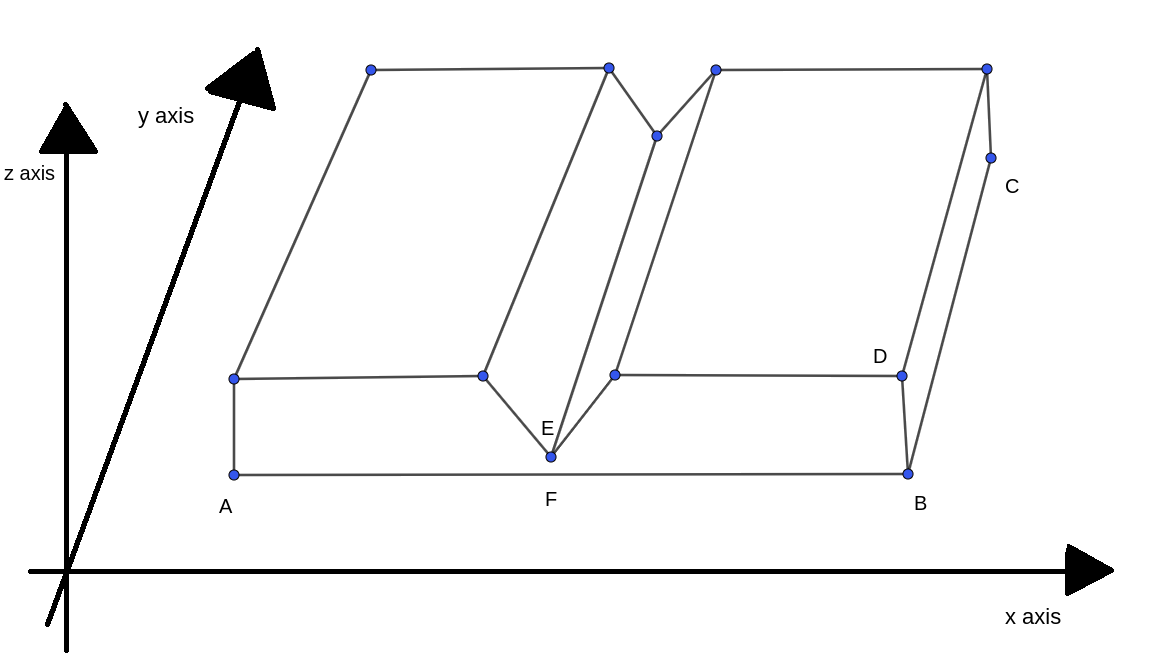
\includegraphics[width=4.5in]{spectralcluster/images/counterexample.png}
\caption{
  The probability density function where $\rho(x, y) =
    \min(\epsilon + x, \frac{1}{n})$ for arbitrary $X, Y, n$.
      Here, $\rho(x,y)$ is plotted in the z axis, and $E$ is at point
      $(0, -Y, \epsilon)$. This function $\rho$ has bad spectral sweep
      cuts when $\alpha = 1, \gamma = 2$.
 }
\label{fig:counterexample}
\end{figure}

We note that this
section combined with Theorem~\ref{thm:sweep-cut},
Lemma~\ref{lem:cheeger-converse} and Lemma~\ref{lem:buser-converse} shows that no Cheeger and Buser
inequality can hold when $\alpha = 1$ and $\gamma = 2$ for any
$\beta$: this section combined with Theorem~\ref{thm:sweep-cut} will
show that the Cheeger-Buser inequalities can only hold for $\beta > 10$,
while Lemma~\ref{lem:cheeger-converse} and Lemma~\ref{lem:buser-converse} shows that they can only hold for
$\beta \leq 1$. Therefore, the Cheeger-Buser inequalities cannot hold for
any $\beta$, for $\alpha = 1$ and $\gamma = 2$.

% See Section~\ref{sec:trade-offs} for more details.

\begin{theorem}\label{thm:counterexample} \textbf{$(\alpha=1,\gamma=2)$-Spectral Sweep Cut Counterexample:}

  For a $1$-Lipschitz positive valued function $\rho$, let $\Phi$ be the
  sparsity of the $(1,3)$-spectral sweep cut, and let $\Phi_{OPT}$ be
  the cut of optimal $(1, \beta)$ sparsity for any $\beta < 10$. There
  there exists a $1$-Lipschitz density function $\rho$ such that:

  \[\Phi > C \max(\Phi_{OPT}, \sqrt{\Phi_{OPT}})\]
  for any constant $C$.
\end{theorem}

\subsection{Our density function}
We first construct our $1$-Lipschitz Density function for which a
$(1,2)$ spectral cut has poor $(1,\beta)$ sparsity. Our density function
has parameters $X, Y, \epsilon, n$ which we will set later.

\begin{definition} Let $\rho: [-X, X] \times [-Y, Y] \rightarrow \mathbb{R}$ be a density function such that:

  \[ \rho(x, y) = \min(\epsilon + x, 1/n) \] 
\end{definition}
To turn this into a $1$-Lipschitz probability density function, we simply
extend it to a function $\rho':\mathbb{R}^2 \rightarrow \mathbb{R}$
where $\rho'$ agrees with $\rho$ on $[-X, X] \times [-Y, Y]$, and the
function goes $1$-Lipschitzly to $0$ outside this range.

We will set $X = \sqrt{n}/10, Y = 10\sqrt{n}$, and $n$ large, to obtain
a density function where the $(1, 2)$ spectral cut has arbitrarily bad
$(1,\beta)$ sparsity for all $\beta < 10$. 

\subsection{Proof Overview}

First, we prove theorems about the zero-set of this density's
$(\alpha=1,\gamma=2)$ eigenfunction. In particular, the zero-set of this
eigenfunction must cut from the line $x=-X$ to $x=X$. It cannot cut from
the line $y = -Y$ to the line $y = Y$.

We prove that any level-set of the eigenfunction can't cut from $y
= -Y$ to $y = Y$. We then show that any cut that doesn't cut from $y =
-Y$ to $y = Y$ has bad $(1,\beta)$ sparsity for $\beta < 10$. This
completes our proof. Moreover, any cut that doesn't cut from $y=-Y$ to
$y=Y$ is intuitively a poor cut of our density function, according to
standard machine learning intuition.

We note the natural cut of this distribution is the straight line cut $x =
0$, which the $(1,3)$-spectral sweep cut will find (this is an artifact
of our proof, though we do not explicitly prove it here).

First, we prove a few lemmas on the zero-set of the $(1,2)$
eigenfunction.
\subsection{The Zero-set of a principal $(1,2)$ eigenfunction is the
line $y = 0$} 

\begin{theorem} \label{thm:zero-set} The Zero-set of the eigenfunction for our given density
  function, is the line $y = 0$.
\end{theorem}
\begin{lemma} Let $f$ be any eigenfunction of our given density function,
  for which $f(x,y) \not= f(x, y')$ for some $x, y \not= y'$. Then
  
  \[ \int_0^Y f(x,y) dy  = 0. \]
\end{lemma}

\begin{lemma}\label{lem:symmetry} There exists a principal eigenfunction $f_2$ of our given
  density function, for which 

  \[f_2(x,y) = f_2 (-x, y) = -f_2(x,-y)\]

\end{lemma}

\begin{proof} This follows from a (non-trivial) symmetrization argument put forward in
  the graph case in Guattery and Miller~\cite{GuMi95}.
\end{proof}

\begin{lemma}\label{lem:nodal} (Nodal domains for Densities) Every principal eigenfunction $f_2$ of our given density
  function satisfies: the closure of the set $\{S = (x,y) | f_2(x,y)
  > 0\}$ is connected.
\end{lemma}
\begin{proof} This follows analogously to the proof of Fiedler's nodal
  domains for eigenfunctions of a graph~\cite{Fiedler73}.
\end{proof}

  \begin{lemma}  \label{lem:pos-neg} Let $f$ be a $(\alpha, \beta)$ eigenfunction of any density function
  supported on a compact set $S \subset \mathbb{R}^n$ for some $n$.
  For every point in the zero-set, if any open set containing that point
  contains a positive element, it must also contain a negative element.
\end{lemma}
\begin{proof}
  This follows directly from the definition of eigenfunction.
\end{proof}

  \begin{proof} (of Theorem~\ref{thm:zero-set}):
    First, we note that there is a principal eigenfunction whose zero
    set contains $y = 0$, by Lemma~\ref{lem:symmetry}. We claim there is a principal
    eigenfunction for which this is the entire zero-set. This follows
    from Lemma~\ref{lem:nodal} and Lemma~\ref{lem:pos-neg}.
  \end{proof}

%% TIM ENDED HERE.

\subsection{Any spectral sweep cut has high $(1,\beta)$ sparsity}
In this section, we prove that the spectral sweep cut must have high $(1,\beta)$-sparsity
for $0 < \beta < 10$, and for $\beta>10$ the spectral sweep-cut either
has high $(1,\beta)$ sparsity or else divides the probability density
into two pieces, one of which has less than $\leq 1/n$ fraction
of the probability mass. 

\begin{lemma}~\label{lem:not-vertical} Any spectral sweep cut (of the principal $(1,2)$
  eigenfunction whose eigenvector's zero-set is the line $y = 0$) can't cut through $y=Y$ and $y =
  -Y$.
\end{lemma}
\begin{proof} 
  This is clear.
\end{proof}
\begin{lemma}\label{lem:notsparse} Any cut that doesn't cut through both $y=Y$ and $y=-Y$ has
  poor $(1,\beta)$ sparsity for any $0 < \beta < 10$. For $\beta > 10$,
  a cut of good $(1,\beta)$ sparsity must have its smaller side contain $o_n(1)$ fraction of the
  mass. 
  
  To be precise, if $\Phi_{\beta}$ is the optimal $(1,\beta)$
  sparsity of the cut, and $\Phi$ is the $(1,\beta)$ sparsity induced by
  a cut that doesn't cut both $y=Y$ and $y=-Y$, then there is no
  constant $C$ independent of $n$ for which

  $\Phi^2 <  C \Phi_\beta $.
\end{lemma}
We note that Theorem~\ref{thm:counterexample} follows from
Lemma~\ref{lem:not-vertical} and~\ref{lem:notsparse}. Thus, it remains
to show Lemma~\ref{lem:notsparse}.

\begin{proof} (of Lemma~\ref{lem:notsparse}). We split this into two
  cases. Consider the side of the level set cut with smaller probability
  mass. The first case is when this side has at least half its
  probability mass outside the region $|x| < 1/n-\epsilon$. The second case is when
  the side has less than half its mass in this region.

  In the first case, we note that we can lower bound the cut by its
  projection onto the $x$ axis. A quick calculation shows that when $X =
  \frac{1}{10\sqrt{n}}$ and $Y = \frac{10}{\sqrt{n}}$, the $(1,
  \beta)$-sparsity of this cut is within a factor of $2$ of the $(1,
  \beta)$-sparsity of the cut $y = 0$ through the uniform distribution of height
  $\frac{1}{n}$ supported on $[-X, X] \times [-Y, Y]$. This $(1, \beta)$
  sparsity is 
  \[ A:= O(\frac{X}{n^\beta}) = O(\frac{\sqrt{n}}{n^\beta})
  \].

  When $\epsilon$ is chosen to be $\frac{1}{n^2\sqrt{n}}$, then the
  $(1,\beta)$ sparsity of the optimal cut is the cut $x=0$, which has
  $(1,\beta)$ sparsity of:
  \[B:= O(\frac{Y}{(n\sqrt{n})^\beta}) =
  O(\frac{\sqrt{n}}{(n^2\sqrt{n})^\beta}.\]

  We note that this choice of $\epsilon$ is the minimum such choice such
  that the principal eigenvector is not constant on the $Y$ axis.

  Now we note that $A^2/B$ goes to infinity as $n$ gets large, if and
  only if

  \[ n^{2\beta} \sqrt{n}^\beta n / n^{2\beta} \sqrt{n} \] goes to infinity,

  or 
  \[ \sqrt{n} (\sqrt{n}^\beta)\] goes to infinity. This is true for any
  $\beta > 0$. This proves Theorem~\ref{thm:counterexample} in case $1$,
  where at least half of the probability mass is outside the region $|x|
  < 1/n$.

  In case $2$, we consider the  case when the smaller side of the cut
  has more than half its probability mass inside the region $|x| < 1/n
  -\epsilon$, which we note is a very small portion of the probability
  mass of the overall probability density. In
  this case, it turns out that we need $\beta < 10$ to give isoperimetry
  guarantees, since for any $\beta > 10$, it turns out that even cuts
  containing small probability mass are considered to have good
  $(1,\beta)$ sparsity, since for large $\beta$, $(1,\beta)$ sparse cuts
  tremendously favor small cuts, even if the smaller side has negligible
  probability mass.

  Since at least half the mass is inside the
  region $|x| < 1/n$, we can assume without loss of generality that the
  entire probability mass of the smaller side of the cut is inside this region, by simply projecting
  the cut onto this region (reducing its $\beta$-perimeter while
  decreasing probability mass by at most a factor of $2$). We can again
  use a symmetry argument analogous to~\ref{lem:symmetry} to show that
  any level set of this principal eigenfunction is symmetric about the
  $x$ axis (we note Lemma~\ref{lem:notsparse} is slightly stronger than
  this as it does not assume symmetry, but for our purposes we can
  strictly deal with symmetric cuts, and the non-symmetric case follows
  through a similar argument). 

  Now given the cut is symmetric about the $x$ axis, if the cut cuts
  through $(x',y')$, then it also cuts through $(-x',y')$, and we can lower
  bound the probability mass contained by the cut $y = y'$ with $x'
  \cdot \rho(x',y')$. A simple calculation using this estimate finishes
  the proof for us.


\end{proof}




%%%%%%%%%%%%%%%% OLD TEXT %%%%%%%%%%%%%%%%%%%%%%
% To prove that the continuous version of classical spectral clustering
% fails to find a $(1, \beta)$-sparse cut, we first establish structure
% about one of the principal eigenvector. In particular, we will show that there
% is a principal eignevector whose $0$-set has a nice structure: it will cut from
% $y=0$ to $y=X$, while the $0$-set cannot touch both $x = 0$ and $x=X$.
% We will show that a cut with the $0$-set as threshold will lead to a
% poor $(1,\beta)$-sparsity.
% Note that a spectral sweep-cut using any threshold $t$ must be contained
% strictly on either side of the cut, and thus cannot touch the two lines
% $x=0$ and $x=X$ simultaneously. We will then prove:
% 
% \begin{lemma} For the density function shown in
%   figure~\ref{fig:counterexample}, any cut that does not touch $x=0$ and
%   $x=X$ simultaneously must have $(1,\beta)$ sparsity of at most
%   $\epsilon^\beta n$ for all $\epsilon < 1/n$.
% \end{lemma}
% \begin{lemma} For $X = \Theta(Y)$, The optimal cut of the density function shown in
%   figure~\ref{fig:counterexample} has $(1,\beta)$ sparsity of
%   $\Theta(\epsilon^\beta \sqrt{n})$.
% \end{lemma}
% \begin{lemma} For $X = 10\sqrt{n}$, $Y = \sqrt{n}$, and $\epsilon \geq 
%   \frac{1}{n^2 \sqrt{n}}$, the principal $(\alpha=1,
%   \gamma=2)$-eigenfunction of the density funciton defined in
%   Definition~\ref{FOO2} has eigenvalue greater than $Q$.\tim{Define $Q$}.
% \end{lemma}
% 
% 
% \subsection{The principal Eigenvector's $0$-set cuts from $x = 0$ to $x
% = X$}
% 
% \subsection{The principal Eigenvector's $0$-set does not touch both $y =
% 0$ and $y=Y$}
% 
% \subsection{Any cut contained entirely within one side of the $0$-set
% has high $(1,\beta)$-sparsity}

% \section{The Effects of Changing $\beta$ on $(1,\beta)$-sparse cuts}
\label{sec:changing-beta}

\section{Conclusion and Future Directions}\label{sec:conclusion}
We define a new notion of spectral sweep cuts, eigenvalues,
Rayleigh quotients, and sparsity for probability densities. We
present the first known Cheeger and Buser inequality on Lipschitz
probability density functions, and use this to show an
$(\alpha=1, \gamma=3)$ spectral
sweep cut on a $L$-Lipschitz probability density function has
provably low $(\alpha=1,\gamma=2)$-sparsity. This work is the first spectral sweep
cut algorithm on non-parametric probability densities with any guarantees on the cut quality.

Further, we show that existing spectral sweep cut methods (such
as those implicit in spectral clustering) compute
$(1, 1)$ or $(1,2)$ spectral sweep cuts, neither of which
has any sparsity guarantees. We prove that $(1,2)$ spectral sweep
cuts, which are implicitly used in traditional spectral
clustering, can lead to undesirable partitions of simple 
$1$-Lipschitz probability densities. Meanwhile, our work showed
that using $(1,3)$ spectral sweep cuts give provably good $(1,2)$
sparse cuts.

For future directions, we conjecture that $\beta =
\alpha+1$ and $\gamma = \alpha+2$ is the only settings of
$(\alpha, \beta, \gamma)$ in which both Cheeger and Buser
inequalities are provable. This would be a stronger theorem than
we currently have for Lemma~\ref{lem:cheeger-converse} and
Lemma~\ref{lem:buser-converse}.

In the Buser inequality, we would like to iron out the exact dimensional
dependence on the dimension,
$d$ (Theorem~\ref{thm:buser_n}). The
authors believe that this dependence can be
reduced to $\sqrt{d}$. It is an open question whether
\textit{any}
dimension dependence is required.  In particular, the latest
version of
Buser's inequality for manifolds has no dimension
dependence~\cite{ledoux2004spectral}. It is an open question how to
generalize their techniques into the density setting, as the
Bochner formula does not easily generalize to densities.

Another open question is whether multi-way Cheeger and Buser inequalities
can be proven on densities, mirroring the work on
graphs~\cite{Louis12, kw16, LeeMultiway14, Lee2014}. This would
allow our clustering algorithms to generalize into $k$-way
clusterings. We additionally would like to know whether one can
understand \textbf{balanced cuts} on proability densities for our
new definitions of sparsity. Balanced cuts in this setting may
have applications to machine learning.

Finally, we would like to know whether Buser and Cheeger inequalities may exist for $L$-Lipschitz
probability densities supported on manifolds with bounded
curvature. If true, this would fully generalize the work
of Cheeger and Buser on manifolds, which may lead to deeper
insight into manifold theory. Moreover, it could have
foundational impact:
a fundamental assumption underlying modern machine learning is
that most data comes from probability density supported on a manifold, and a Cheeger and Buser inequality in this
setting would give provable sparsity guarantees about
spectral sweep cuts in this setting.

%\bibliographystyle{alpha}
%\bibliography{123}
%\appendix
\begin{appendix}
  \section{Calculating Eigenvalues and Isoperimetry constants for Simple
  Examples}\label{app:examples}
Recall from Section~\ref{sec:examples} the definitions of $\rho_1$ and
$\rho_2$. This section is devoted to computing the eigenvalues and
isoperimetric constants of these densities. We note that the eigenvalue
and isoperimetry computation for $\rho_1$ is straightforward, so we omit
it. The isoperimetry constant for $\rho_2$ is also straightforward, as
the isoperimetric cut will be at $x = 0$. The only non-trivial
computation is the $(\alpha,\beta)$-eigenvalue for $\rho_2$.

\subsection{Notation}
We will write $a\gtrsim b$ if $a\geq cb$ for some absolute constant $0<c<\infty$. Similarly define $a \lesssim b$. We will write $a\asymp b$ if both relations hold.

\subsection{A Lipschitz weight}
\label{subsec:lipschitz_example}

It is clear that
\begin{align*}
\Phi \asymp \epsilon^\beta.
\end{align*}
Next, we apply the Hardy-Muckenhoupt inequality~\cite{MillerHardy18} to estimate $\lambda_2$
for $\rho_2$. 

We upper bound $\H$ as:

\begin{align*}
\H &\leq\R(1)\M(0)\\
  &\asymp  \int_0^1 \frac{1}{(x+\epsilon)^{\gamma}}\,dx\\
& \lesssim \begin{cases}
  1 & \text{if } \gamma<1\\
  \ln\left(1/\epsilon\right)& \text{if } \gamma = 1\\
  O\epsilon^{1-\gamma}& \text{if } \gamma>1.
\end{cases}
\end{align*}
By the Hardy-Muckenhoupt inequality, we can lower bound $\lambda_2$ with
the inverse of an upper bound on $\H$. Thus, as claimed in
Section~\ref{sec:examples}, we can lower bound $\lambda_2$ with
$\epsilon^{\gamma - 1}$ when $\gamma \geq 1$.

Thus, if we want a Buser-type inequality to hold, then $(\alpha,\beta,\gamma)$ needs to satisfy,
\begin{align*}
\begin{cases}
  1\lesssim \lambda_2 \lesssim \max(\Phi,\Phi^2)  \asymp \epsilon^\beta & \text{if } \gamma<1\\
  \frac{1}{\ln\left(1/\epsilon\right)}\lesssim \lambda_2 \lesssim \max(\Phi,\Phi^2)  \asymp \epsilon^\beta& \text{if } \gamma = 1\\
  \epsilon^{\gamma-1}\lesssim \lambda_2 \lesssim \max(\Phi,\Phi^2)  \asymp \epsilon^\beta& \text{if } \gamma>1.
\end{cases}
\end{align*}
By letting $\epsilon$ go to zero, it is clear that $\gamma-1\geq \beta$,
   as desired.


  \section{Cheeger and Buser for Density Functions does not easily follow
  from Graph or Manifold Cheeger and Buser}\label{app:notgraph}

\subsection{Comments on Graph Cheeger-Buser}
The most natural method of proving distributional Cheeger-Buser
inequality using the graph Cheeger-Buser inequality is to
generate a vertex and edge weighted graph approximating the distribution, and write down
graph Cheeger-Buser. Then, one would generate a sequence of graphs with
an increasing number of vertices. Ideally, the graph Cheeger-Buser inequality
on these graphs would converge to a
Cheeger-Buser inequality on the underlying distribution. This
discretization approach follows a standard paradigm of
approximating distributions with graphs, present in
numerical methods, finite element methods,
         and machine learning
         ~\cite{TrillosRate15,TrillosVariational15,SPIELMAN2007284}.

Such an approach cannot work (no matter how the
    eigenvalues and isoperimetric cuts are defined for
    distributions). The easiest way to see this is to attempt to execute
    this strategy for a simple uniform distribution in $1$ dimension, on
    the interval $[0,1]$. One would naively approximate this
    distribution
    with a line graph with $n$ vertices, with edge weights $w_n$ and vertex
    weights $m_n$. Then one would take $n$ to go to infinity.

    If one writes down the Cheeger and Buser inequalities for graphs in
    this example, we get:
    
    \[\frac{w_n}{m_n n^2} \leq \Phi_{OPT} \leq \frac{w_n}{m_n n} \]

    No matter what $m_n$ and $w_n$ are, the ratio between the upper and
    lower bound is $n$, which diverges. Thus, either the Cheeger
    inequality or the Buser inequality becomes meaningless: either the
    lower bound goes to $0$ or the upper bound goes to $\infty$, or
    both, depending on
    how $w_n$ and $m_n$ are set.

    Thus, even for the simple case of a uniform distribution on $[0,1]$
    the natural strategy for deriving probability density Cheeger/Buser
    from graph Cheeger/Buser fails.

\subsection{Comments on Manifold Cheeger-Buser}
Distributional Buser does not easily follow from an
application of
the manifold Buser inequality. We recall that manifold Buser only applies for
    manifolds with bounded Ricci curvature. The natural way to parlay manifold Buser into
distributional Buser on $\RR^d$ is to change the underlying metric tensor
on $\RR^d$ to factor in the probability density function at that
point. However, the authors are unaware of any method of doing
this for which one can recover a meaningful Cheeger and
Buser inequality. Moreover, it is unclear how to obtain any Ricci
curvature bounds when we change the metric tensor.

Most modern approaches to proving Buser's inequality for
    manifolds rely on the
Li-Yau inequality, which in turn depends on the Bochner identity
    for manifolds on bounded Ricci
    curvature~\cite{ledoux2004spectral}.
The authors are unaware of a clean Bochner-like identity for
distributions. Older techniques use Almgren's minimizing currents
and/or Epsilon nets~\cite{Buser82}. For the former, we do not know of any
analog for distributions. For the latter, the corresponding
Buser inequality has a $2^{d}$ multiplicative dependence, which
is significantly worse than our $d$ dependence.

  %!TEX root = ms.tex

\section{A weighted Cheeger inequality in one dimension}
\label{sec:one_dim}
\begin{theorem}
\label{thm:cheeger_1}
Let $\Omega = (a,b)$ where $-\infty<a<b<\infty$. Let $\rho:(a,b)\to\RR_{>0}$ be Lipschitz continuous. Then,
\begin{align*}
\Phi(\Omega)^{2} &\leq 4\norm{\rho^{\beta - \frac{\alpha+\gamma}{2}}}^2_\infty\lambda_2(\Omega).
\end{align*}
In particular, when $(\alpha,\beta,\gamma) = (1,2,3)$, we have
\begin{align*}
\Phi(\Omega)^2\leq 4\lambda_2(\Omega).
\end{align*}
\end{theorem}
\begin{proof}
Let $w\in W^{1,2}(\Omega) \cap C^\infty(\Omega)$ be a strictly decreasing function with $\int_\Omega\rho^\alpha w\,dx = 0$.
Let $v = w + a1$ where $a$ is chosen such that
$\abs{\set{v<0}}_\alpha = \abs{\set{v>0}}_\alpha$.
Note that
\begin{align*}
R(w) &= \frac{\int_\Omega \rho^\gamma (w')^2\,dx}{\int_\Omega \rho^\alpha w^2\,dx}\\
&\geq \frac{\int_\Omega \rho^\gamma (w')^2\,dx}{\int_\Omega \rho^\alpha w^2\,dx + a^2 \abs{\Omega}_\alpha}\\
&= R(v).
\end{align*}
Let $\hat x\in(a,b)$ be the unique value such that $v(\hat x) = 0$. Without loss of generality, the function $u= \max(v,0)$ satisfies $R(u)\leq R(v)$ and has $u(a)= 1$.

Let $g = u^2$. Noting that $g' = 2uu'$ a.e., we can apply Cauchy-Schwarz to obtain
\begin{align*}
\int_a^{\hat x} \rho^\beta \abs{g'}\,dx
&= 2\int_a^{\hat x} \rho^\beta \abs{u}\abs{u'}\,dx\\
&\leq 2\sqrt{\int_a^{\hat x} \rho^{2\beta-\alpha} (u')^2\,dx}\sqrt{\int_a^{\hat x} \rho^\alpha u^2\,dx}\\
&\leq 2\norm{\rho^{\beta - \frac{\alpha+\gamma}{2}}}_\infty\sqrt{\int_a^{\hat x} \rho^\gamma (u')^2\,dx}\sqrt{\int_a^{\hat x} \rho^\alpha u^2\,dx}.
\end{align*}
Then, dividing by $\int_a^{\hat x} \rho^\alpha g\,dx$, we have
\begin{align*}
\frac{\int_a^{\hat x} \rho^\beta \abs{g'}\,dx}{\int_a^{\hat x} \rho^\alpha g\,dx} &\leq 2\norm{\rho^{\beta - \frac{\alpha+\gamma}{2}}}_\infty\sqrt{ R(w)}.
\end{align*}
By change of variables,
\begin{align*}
\int_a^{\hat x} \rho^\beta \abs{g'}\,dx &= \int_{0}^{1} \rho^\beta(g^{-1}(t))\,dt.
\end{align*}
Writing $g(x) = \int_0^{g(x)} 1\,dt$ and applying Tonelli's theorem, we rewrite the denominator
\begin{align*}
\int_a^{\hat x} \rho^\alpha g\,dx &= \int_{0}^{1}\abs{(a,g^{-1}(t))}_\alpha\,dt.
\end{align*}
Thus, by averaging, there exists some $t^*$ such that,
\begin{align*}
\Phi(\Omega) &\leq \frac{\rho^\beta(t^*)}{\abs{(a,t^*)}_\alpha}
\leq \frac{\int_a^{\hat x}\rho^\beta \abs{g'}\,dx}{\int_a^{\hat x}\rho^\alpha g\,dx}
\leq 2\norm{\rho^{\beta - \frac{\alpha+\gamma}{2}}}_\infty\sqrt{R(w)}.
\end{align*}g
% Applying Lemma \ref{lem:c_infty_dense} completes the proof.
\end{proof}

\begin{theorem}
\label{thm:buser_1}
Let $\Omega = (a,b)$ where $-\infty<a<b<\infty$. Let $\rho:(a,b)\to\RR_{>0}$ be Lipschitz continuous with Lipschitz constant $L$. Then,
\begin{align*}
\lambda_2(\Omega) &\leq 8\cdot (3/2)^{\gamma/\alpha} \norm{\rho^{\gamma -1 - \beta}}_\infty \max\left(4\norm{\rho^{\alpha+1-\beta}}_\infty \Phi^2(\Omega), \frac{\alpha}{\ln(3/2)}L\Phi(\Omega)\right).
\end{align*}
In particular, when $(\alpha,\beta,\gamma) = (1,2,3)$, we have
\begin{align*}
\lambda_2(\Omega) &\leq O\left(\max\left(\Phi^2(\Omega), L\Phi(\Omega)\right)\right).
\end{align*}
\end{theorem}
\begin{proof}
Let $\hat x\in(a,b)$. We will show that there exists a $u\in W^{1,2}(\Omega)$ with small Rayleigh quotient compared to $\Phi(\hat x)$.
Let $A = (a,\hat x)$ and $B = (\hat x, b)$. Without loss of generality $\abs{A}_\alpha \leq \abs{B}_\alpha$ and hence $\Phi(\hat x) = \frac{\rho^\beta (\hat x)}{\abs{A}_\alpha}$. For notational convenience, we will write $\Phi = \Phi(\hat x)$ in this proof.

Let
\begin{align*}
u(x) = \begin{cases}
	\abs{A}_\alpha & a \leq x \leq \hat x\\
	-\abs{B}_\alpha & \hat x < x\leq b.
\end{cases}
\end{align*}
Let $\delta=\theta \rho(\hat x)$ where $\theta>0$ will be picked later. Define the continuous function
\begin{align*}
u_\delta(x) = \begin{cases}
	\abs{A}_\alpha & a \leq x \leq x_1\\
	\text{linear with slope }\frac{-\abs{\Omega}_\alpha}{\delta} & x_1 \leq x \leq x_2\\
	-\abs{B}_\alpha & x_2 \leq x \leq b
\end{cases}
\end{align*}
where $a\leq x_1<\hat x< x_2\leq b$ are picked such that $\int_a^b \rho^\alpha u_\delta\,dx = 0$. Note $x_2 - x_1\leq \delta$.

We bound the numerator in $R(u_\delta)$ using the mean value theorem.
\begin{align*}
\int_a^b \rho^\gamma (u_\delta')^2\,dx  &= \frac{\abs{\Omega}_\alpha^2}{\delta^2}\int_{x_1}^{x_2}\rho^\gamma \,dx\\
&\leq \frac{\abs{\Omega}_\alpha^2}{\delta}\rho^\gamma(\tilde x)\hspace{2em}\text{for some }\tilde x \in[x_1,x_2]\\
&\leq \abs{\Omega}_\alpha^2\rho^{\gamma-1}(\hat x)(1+L\theta)^\gamma/\theta
\end{align*}
In the third line we used the Lipschitz estimate $\rho(\tilde x) \leq \rho(\hat x)(1+L\theta)$.
We lower bound the denominator in $R(u_\delta)$ using the mean value theorem and the same Lipschitz estimate. We will also recall that $\Phi = \rho^\beta(\hat x)/\abs{A}_\alpha$.
\begin{align*}
\int_a^b \rho^\alpha u_\delta^2\,dx &\geq \int_a^b \rho^\alpha u^2\,dx - \int_{x_1}^{x_2}  \rho^\alpha u^2\,dx\\
&\geq \abs{A}_\alpha\abs{B}_\alpha\abs{\Omega}_\alpha - \delta\rho^\alpha(\tilde x)\abs{B}_\alpha^2\hspace{2em}\text{for some }\tilde x \in[x_1,x_2]\\
&\geq \abs{A}_\alpha\abs{B}_\alpha\abs{\Omega}_\alpha - \rho^{\alpha+1}(\hat x)\abs{B}_\alpha^2(1+L\theta)^\alpha\theta\\
&\geq \abs{\Omega}_\alpha^2\left(\abs{A}_\alpha/2 - \rho^{\alpha+1}(\hat x) (1+L\theta)^\alpha \theta\right)\\
&\geq \abs{\Omega}_\alpha^2\abs{A}_\alpha\left(1/2 - \norm{\rho^{\alpha+1-\beta}}_\infty \Phi (1+L\theta)^\alpha \theta\right)
\end{align*}
The parameter $\theta$ will be chosen such that the estimate of the denominator is positive.
We combine the two bounds above.
\begin{align*}
R(u_\delta)
&\leq \frac{\abs{\Omega}_\alpha^2\rho^{\gamma-1}(\hat x)(1+L\theta)^\gamma/\theta}{\abs{\Omega}_\alpha^2\abs{A}_\alpha\left(1/2 - \norm{\rho^{\alpha+1-\beta}}_\infty \Phi (1+L\theta)^\alpha \theta\right)}\\
&= \frac{\rho^{\gamma-1-\beta}(\hat x)\Phi(1+L\theta)^\gamma/\theta}{1/2 - \norm{\rho^{\alpha+1-\beta}}_\infty \Phi (1+L\theta)^\alpha \theta}\\
&\leq \frac{\norm{\rho^{\gamma -1 - \beta}}_\infty\Phi(1+L\theta)^\gamma/\theta}{1/2 -\norm{\rho^{\alpha + 1 - \beta}}_\infty\Phi(1+L\theta)^\alpha\theta}.
\end{align*}

We make the following choice of $\theta>0$,
\begin{align*}
\theta = \min\left(\frac{1}{4\Phi\norm{\rho^{\alpha+1-\beta}}_\infty}, \frac{\ln(3/2)}{\alpha L} \right).
\end{align*}
Then, $(1+L\theta)\leq (3/2)^{1/\alpha}$ and $\Phi\theta \leq \frac{1}{4\norm{\rho^{\alpha+1-\beta}}_\infty}$. Thus,
\begin{align*}
\lambda_2 &\leq R(u_\delta)\\
&\leq 8\cdot (3/2)^{\gamma/\alpha} \norm{\rho^{\gamma -1 - \beta}}_\infty \frac{\Phi}{\theta}\\
&= 8\cdot (3/2)^{\gamma/\alpha} \norm{\rho^{\gamma -1 - \beta}}_\infty \max\left(4\norm{\rho^{\alpha+1-\beta}}_\infty \Phi^2, \frac{\alpha}{\ln(3/2)}L\Phi\right).
\end{align*}
Finally, picking $\hat x$ such that $\Phi(\hat x)\to \Phi(\Omega)$ completes the proof.
\end{proof}

\begin{remark}
Recall the example presented in Section~\ref{subsec:lipschitz_example}, i.e. $\Omega = (-1,1)$, $\rho = \abs{x}+\epsilon$. For the choice $(\alpha,\beta,\gamma) = (1,1,1)$, it was shown that $\frac{\lambda_2(\Omega)}{\Phi(\Omega)^{p}}$ diverges to infinity as $\epsilon\to 0$ for any $p>0$. This does not contradict our Theorem~\ref{thm:buser_1}, which only asserts that
\begin{align*}
\lambda_2(\Omega) &\lesssim \frac{1}{\epsilon}\max\left(\Phi^{2}(\Omega),\Phi(\Omega)\right).
\end{align*}
\end{remark}

%  %!TEX root = ms.tex

\section{A weighted Cheeger inequality in one dimension}
\label{sec:one_dim}
\begin{theorem}
\label{thm:cheeger_1}
Let $\Omega = (a,b)$ where $-\infty<a<b<\infty$. Let $\rho:(a,b)\to\RR_{>0}$ be Lipschitz continuous. Then,
\begin{align*}
\Phi(\Omega)^{2} &\leq 4\norm{\rho^{\beta - \frac{\alpha+\gamma}{2}}}^2_\infty\lambda_2(\Omega).
\end{align*}
In particular, when $(\alpha,\beta,\gamma) = (1,2,3)$, we have
\begin{align*}
\Phi(\Omega)^2\leq 4\lambda_2(\Omega).
\end{align*}
\end{theorem}
\begin{proof}
Let $w\in W^{1,2}(\Omega) \cap C^\infty(\Omega)$ be a strictly decreasing function with $\int_\Omega\rho^\alpha w\,dx = 0$.
Let $v = w + a1$ where $a$ is chosen such that
$\abs{\set{v<0}}_\alpha = \abs{\set{v>0}}_\alpha$.
Note that
\begin{align*}
R(w) &= \frac{\int_\Omega \rho^\gamma (w')^2\,dx}{\int_\Omega \rho^\alpha w^2\,dx}\\
&\geq \frac{\int_\Omega \rho^\gamma (w')^2\,dx}{\int_\Omega \rho^\alpha w^2\,dx + a^2 \abs{\Omega}_\alpha}\\
&= R(v).
\end{align*}
Let $\hat x\in(a,b)$ be the unique value such that $v(\hat x) = 0$. Without loss of generality, the function $u= \max(v,0)$ satisfies $R(u)\leq R(v)$ and has $u(a)= 1$.

Let $g = u^2$. Noting that $g' = 2uu'$ a.e., we can apply Cauchy-Schwarz to obtain
\begin{align*}
\int_a^{\hat x} \rho^\beta \abs{g'}\,dx
&= 2\int_a^{\hat x} \rho^\beta \abs{u}\abs{u'}\,dx\\
&\leq 2\sqrt{\int_a^{\hat x} \rho^{2\beta-\alpha} (u')^2\,dx}\sqrt{\int_a^{\hat x} \rho^\alpha u^2\,dx}\\
&\leq 2\norm{\rho^{\beta - \frac{\alpha+\gamma}{2}}}_\infty\sqrt{\int_a^{\hat x} \rho^\gamma (u')^2\,dx}\sqrt{\int_a^{\hat x} \rho^\alpha u^2\,dx}.
\end{align*}
Then, dividing by $\int_a^{\hat x} \rho^\alpha g\,dx$, we have
\begin{align*}
\frac{\int_a^{\hat x} \rho^\beta \abs{g'}\,dx}{\int_a^{\hat x} \rho^\alpha g\,dx} &\leq 2\norm{\rho^{\beta - \frac{\alpha+\gamma}{2}}}_\infty\sqrt{ R(w)}.
\end{align*}
By change of variables,
\begin{align*}
\int_a^{\hat x} \rho^\beta \abs{g'}\,dx &= \int_{0}^{1} \rho^\beta(g^{-1}(t))\,dt.
\end{align*}
Writing $g(x) = \int_0^{g(x)} 1\,dt$ and applying Tonelli's theorem, we rewrite the denominator
\begin{align*}
\int_a^{\hat x} \rho^\alpha g\,dx &= \int_{0}^{1}\abs{(a,g^{-1}(t))}_\alpha\,dt.
\end{align*}
Thus, by averaging, there exists some $t^*$ such that,
\begin{align*}
\Phi(\Omega) &\leq \frac{\rho^\beta(t^*)}{\abs{(a,t^*)}_\alpha}
\leq \frac{\int_a^{\hat x}\rho^\beta \abs{g'}\,dx}{\int_a^{\hat x}\rho^\alpha g\,dx}
\leq 2\norm{\rho^{\beta - \frac{\alpha+\gamma}{2}}}_\infty\sqrt{R(w)}.
\end{align*}g
% Applying Lemma \ref{lem:c_infty_dense} completes the proof.
\end{proof}

\begin{theorem}
\label{thm:buser_1}
Let $\Omega = (a,b)$ where $-\infty<a<b<\infty$. Let $\rho:(a,b)\to\RR_{>0}$ be Lipschitz continuous with Lipschitz constant $L$. Then,
\begin{align*}
\lambda_2(\Omega) &\leq 8\cdot (3/2)^{\gamma/\alpha} \norm{\rho^{\gamma -1 - \beta}}_\infty \max\left(4\norm{\rho^{\alpha+1-\beta}}_\infty \Phi^2(\Omega), \frac{\alpha}{\ln(3/2)}L\Phi(\Omega)\right).
\end{align*}
In particular, when $(\alpha,\beta,\gamma) = (1,2,3)$, we have
\begin{align*}
\lambda_2(\Omega) &\leq O\left(\max\left(\Phi^2(\Omega), L\Phi(\Omega)\right)\right).
\end{align*}
\end{theorem}
\begin{proof}
Let $\hat x\in(a,b)$. We will show that there exists a $u\in W^{1,2}(\Omega)$ with small Rayleigh quotient compared to $\Phi(\hat x)$.
Let $A = (a,\hat x)$ and $B = (\hat x, b)$. Without loss of generality $\abs{A}_\alpha \leq \abs{B}_\alpha$ and hence $\Phi(\hat x) = \frac{\rho^\beta (\hat x)}{\abs{A}_\alpha}$. For notational convenience, we will write $\Phi = \Phi(\hat x)$ in this proof.

Let
\begin{align*}
u(x) = \begin{cases}
	\abs{A}_\alpha & a \leq x \leq \hat x\\
	-\abs{B}_\alpha & \hat x < x\leq b.
\end{cases}
\end{align*}
Let $\delta=\theta \rho(\hat x)$ where $\theta>0$ will be picked later. Define the continuous function
\begin{align*}
u_\delta(x) = \begin{cases}
	\abs{A}_\alpha & a \leq x \leq x_1\\
	\text{linear with slope }\frac{-\abs{\Omega}_\alpha}{\delta} & x_1 \leq x \leq x_2\\
	-\abs{B}_\alpha & x_2 \leq x \leq b
\end{cases}
\end{align*}
where $a\leq x_1<\hat x< x_2\leq b$ are picked such that $\int_a^b \rho^\alpha u_\delta\,dx = 0$. Note $x_2 - x_1\leq \delta$.

We bound the numerator in $R(u_\delta)$ using the mean value theorem.
\begin{align*}
\int_a^b \rho^\gamma (u_\delta')^2\,dx  &= \frac{\abs{\Omega}_\alpha^2}{\delta^2}\int_{x_1}^{x_2}\rho^\gamma \,dx\\
&\leq \frac{\abs{\Omega}_\alpha^2}{\delta}\rho^\gamma(\tilde x)\hspace{2em}\text{for some }\tilde x \in[x_1,x_2]\\
&\leq \abs{\Omega}_\alpha^2\rho^{\gamma-1}(\hat x)(1+L\theta)^\gamma/\theta
\end{align*}
In the third line we used the Lipschitz estimate $\rho(\tilde x) \leq \rho(\hat x)(1+L\theta)$.
We lower bound the denominator in $R(u_\delta)$ using the mean value theorem and the same Lipschitz estimate. We will also recall that $\Phi = \rho^\beta(\hat x)/\abs{A}_\alpha$.
\begin{align*}
\int_a^b \rho^\alpha u_\delta^2\,dx &\geq \int_a^b \rho^\alpha u^2\,dx - \int_{x_1}^{x_2}  \rho^\alpha u^2\,dx\\
&\geq \abs{A}_\alpha\abs{B}_\alpha\abs{\Omega}_\alpha - \delta\rho^\alpha(\tilde x)\abs{B}_\alpha^2\hspace{2em}\text{for some }\tilde x \in[x_1,x_2]\\
&\geq \abs{A}_\alpha\abs{B}_\alpha\abs{\Omega}_\alpha - \rho^{\alpha+1}(\hat x)\abs{B}_\alpha^2(1+L\theta)^\alpha\theta\\
&\geq \abs{\Omega}_\alpha^2\left(\abs{A}_\alpha/2 - \rho^{\alpha+1}(\hat x) (1+L\theta)^\alpha \theta\right)\\
&\geq \abs{\Omega}_\alpha^2\abs{A}_\alpha\left(1/2 - \norm{\rho^{\alpha+1-\beta}}_\infty \Phi (1+L\theta)^\alpha \theta\right)
\end{align*}
The parameter $\theta$ will be chosen such that the estimate of the denominator is positive.
We combine the two bounds above.
\begin{align*}
R(u_\delta)
&\leq \frac{\abs{\Omega}_\alpha^2\rho^{\gamma-1}(\hat x)(1+L\theta)^\gamma/\theta}{\abs{\Omega}_\alpha^2\abs{A}_\alpha\left(1/2 - \norm{\rho^{\alpha+1-\beta}}_\infty \Phi (1+L\theta)^\alpha \theta\right)}\\
&= \frac{\rho^{\gamma-1-\beta}(\hat x)\Phi(1+L\theta)^\gamma/\theta}{1/2 - \norm{\rho^{\alpha+1-\beta}}_\infty \Phi (1+L\theta)^\alpha \theta}\\
&\leq \frac{\norm{\rho^{\gamma -1 - \beta}}_\infty\Phi(1+L\theta)^\gamma/\theta}{1/2 -\norm{\rho^{\alpha + 1 - \beta}}_\infty\Phi(1+L\theta)^\alpha\theta}.
\end{align*}

We make the following choice of $\theta>0$,
\begin{align*}
\theta = \min\left(\frac{1}{4\Phi\norm{\rho^{\alpha+1-\beta}}_\infty}, \frac{\ln(3/2)}{\alpha L} \right).
\end{align*}
Then, $(1+L\theta)\leq (3/2)^{1/\alpha}$ and $\Phi\theta \leq \frac{1}{4\norm{\rho^{\alpha+1-\beta}}_\infty}$. Thus,
\begin{align*}
\lambda_2 &\leq R(u_\delta)\\
&\leq 8\cdot (3/2)^{\gamma/\alpha} \norm{\rho^{\gamma -1 - \beta}}_\infty \frac{\Phi}{\theta}\\
&= 8\cdot (3/2)^{\gamma/\alpha} \norm{\rho^{\gamma -1 - \beta}}_\infty \max\left(4\norm{\rho^{\alpha+1-\beta}}_\infty \Phi^2, \frac{\alpha}{\ln(3/2)}L\Phi\right).
\end{align*}
Finally, picking $\hat x$ such that $\Phi(\hat x)\to \Phi(\Omega)$ completes the proof.
\end{proof}

\begin{remark}
Recall the example presented in Section~\ref{subsec:lipschitz_example}, i.e. $\Omega = (-1,1)$, $\rho = \abs{x}+\epsilon$. For the choice $(\alpha,\beta,\gamma) = (1,1,1)$, it was shown that $\frac{\lambda_2(\Omega)}{\Phi(\Omega)^{p}}$ diverges to infinity as $\epsilon\to 0$ for any $p>0$. This does not contradict our Theorem~\ref{thm:buser_1}, which only asserts that
\begin{align*}
\lambda_2(\Omega) &\lesssim \frac{1}{\epsilon}\max\left(\Phi^{2}(\Omega),\Phi(\Omega)\right).
\end{align*}
\end{remark}

%  %!TEX root = ms.tex

\section{Higher dimensions}
\label{sec:Ahigher_dim}
In this section the theory of functions of bounded variaion is used to
provide the abstract notions needed to justify certain formal
calculations in the proof of Theorem \ref{:??}.

\begin{definition}
For a measurable set $A\subseteq \Omega$, define
\begin{align*}
\abs{A}_\alpha \coloneqq \int_A \rho^\alpha(x)\,dx.
\end{align*}
\end{definition}
We define the weight of the boundary distributionally~\cite{betta2008weighted,parini2011introduction}.
\begin{definition}
\label{def:betaBdy}
For $A\subseteq\Omega$ a set of finite perimeter, define
\begin{align*}
\abs{\boundary A}_\beta \coloneqq \sup\set{\int_\Omega \chi_A(x) \div(\rho^\beta (x) \phi(x))\,dx\smid \phi\in C_c^1(\Omega),\, \norm{\phi}_{\infty}\leq 1}.
\end{align*}
\end{definition}

\begin{remark}
  This definition corresponds to the intuitive definition of the
  boundary integral of $\rho^\beta$ when $\boundary A$ is sufficiently
  regular.  Specifically, if $A\subseteq\Omega$ has smooth boundary
  and then,
  $$
  \abs{\boundary A}_\beta = \int_{\boundary A} \rho^\beta(x)\,d \mc H^{n-1}(x),
  $$
  where $\mc H^{n-1}$ denotes surface (Hausdorf) measure.
\end{remark}


\begin{definition}
Let $A\subseteq\Omega$ be a set of finite perimeter such that $\abs{A}_\alpha,\abs{\Omega\setminus A}_\alpha >0$. The \textit{isoperimetric ratio} of the cut induced by $A$ is
\begin{align*}
\Phi(A) &\coloneqq \frac{\abs{\boundary A}_\beta}{\min\left(\abs{A}_\alpha,\abs{\Omega\setminus A}_\alpha\right)}
\end{align*}
and the \textit{isoperimetric constant} of $\Omega$ with weight $\rho$ is
\begin{align*}
\Phi(\Omega)\coloneqq \inf_{A\subseteq\overline{\Omega}} \Phi(A).
\end{align*}
Here, $A$ is taken over sets of finite perimeter such that $\abs{A}_\alpha,\abs{\Omega\setminus A}_\alpha>0$.
\end{definition}

Again we define $\lambda_2$ variationally.
\begin{definition}
Let $u\in W^{1,2}(\Omega)$. The \textit{Rayleigh quotient} of $u$ is
\begin{align*}
R(u) &= \frac{\int_\Omega \rho^\gamma\norm{\grad u}^2\,dx}{\int_\Omega \rho^\alpha u^2\,dx}
\end{align*}
and the \textit{second eigenvalue of the Laplacian} on $\Omega$ with weight $\rho$ is
\begin{align*}
\lambda_2(\Omega) &\coloneqq \inf_{u\in W^{1,2}}\set{R(u) \smid \int_\Omega \rho^\alpha u \,dx = 0,\, u\neq 0}.
\end{align*}
\end{definition}

We now prove a weighted Cheeger inequality in higher dimensions. The proof is almost identical to the proof in one dimension. The only change in the proof is replacing the change of variables formula with a coarea formula.
\begin{theorem} \label{thm:Acheeger_n}
Let $\Omega\subseteq\RR^n$ be a bounded convex domain with Lipschitz boundary. Let $\rho:{\Omega}\to\RR_{>0}$ be a Lipschitz function. Then,
\begin{align*}
\Phi^2(\Omega) \leq 4 \norm{\rho^{\beta - \frac{\alpha+\gamma}{2}}}^2_\infty \lambda_2(\Omega).
\end{align*}
In particular, when $(\alpha,\beta,\gamma) = (1,2,3)$ we have
\begin{align*}
\Phi^{2}(\Omega) \leq 4\lambda_2(\Omega).
\end{align*}
\end{theorem}
\begin{proof}
Let $w\in W^{1,2}$ nonzero with $\int_\Omega \rho^\alpha w\,dx = 0$. Let $v = w+a1$ where $a$ is chosen such that $\abs{\set{v<0}}_\alpha = \abs{\set{v>0}}$. Note that
\begin{align*}
R(w) &= \frac{\int_\Omega \rho^\gamma \abs{\grad w}^2\,dx}{\int_\Omega \rho^\alpha w^2\,dx}\\
&\geq \frac{\int_\Omega \rho^\gamma \abs{\grad w}^2\,dx}{\int_\Omega \rho^\alpha w^2\,dx+ a^2\abs{\Omega}_\alpha}\\
&= R(v).
\end{align*}
Without loss of generality, the function $u = \max(v,0)$ satisfies $R(u)\leq R(v)$.

Let $\Omega_0 = \set{v>0}$. Let $g = u^2$. Noting that $\grad g = 2u\grad u$ a.e., we can apply Cauchy-Schwarz to obtain
\begin{align*}
\int_{\Omega_0}\rho^\beta \abs{\grad g}\,dx &= 2\int_{\Omega_0}\rho^\beta \abs{u}\abs{\grad u}\,dx\\
&\leq 2 \sqrt{\int_{\Omega_0} \rho^{2\beta - \alpha} \abs{\grad u}^2\,dx}\sqrt{\int_{\Omega_0} \rho^{\alpha} u^2\,dx}\\
&\leq 2 \norm{\rho^{\beta - \frac{\alpha+\gamma}{2}}}_\infty \sqrt{\int_{\Omega_0} \rho^\gamma \abs{\grad u}^2\,dx}\sqrt{\int_{\Omega_0} \rho^{\alpha} u^2\,dx}.
\end{align*}
Then, dividing by $\int_{\Omega_0} \rho^\alpha g\,dx$, we have
\begin{align*}
\frac{\int_{\Omega_0} \rho^\beta \abs{\grad g}\,dx}{\int_{\Omega_0} \rho^\alpha g\,dx} &\leq2 \norm{\rho^{\beta - \frac{\alpha+\gamma}{2}}}_\infty \sqrt{R(w)}.
\end{align*}
Let $A_t = \set{g>t}$. Then, by the weighted coarea formula,
\begin{align*}
\int_{\Omega_0} \rho^\beta \abs{\grad g}\,dx = \int_0^\infty \abs{\boundary A_t}_\beta\,dt.
\end{align*}
Writing $g(x) = \int_0^{g(x)} 1 \,dt$ and applying Tonelli's thoerem, we rewrite the denominator
\begin{align*}
\int_{\Omega_0} \rho^\alpha g\,dx = \int_{0}^\infty \abs{A_t}_\alpha\,dt.
\end{align*}
Thus, by averaging, there exists some $t^*$ such that
\begin{align*}
\Phi(\Omega) &\leq \Phi(A_{t^*})\\
&\leq \frac{\int_{\Omega_0} \rho^\beta \abs{\grad g}\,dx}{\int_{\Omega_0} \rho^\alpha g\,dx}\\
&\leq2 \norm{\rho^{\beta - \frac{\alpha+\gamma}{2}}}_\infty \sqrt{R(w)}.
\end{align*}
Optimizing over the set $\set{w\in W^{1,2}\smid w\neq 0,\,\int_\Omega \rho^\alpha w\,dx = 0}$ completes the proof.
\end{proof}

We now prove our weighted Buser-type inequality.

\begin{theorem} \label{thm:Abuser_n}
  Let $\Omega\subseteq\RR^n$ be a
  bounded convex domain with Lipschitz boundary. Let
  $\rho:\overline{\Omega}\to\RR_{>0}$ be a Lipschitz function with
  Lipschitz constant $L$. Then,
\begin{align*}
\lambda_2(\Omega) \leq 2 C(\phi,\beta)\linf{\rho^{\gamma-\beta-1}}(1+L) 
  \max\left(L \Phi(A), C(\beta)\linf{\rho^{\alpha+1-\beta}} \Phi(A)^2 \vph\right)
\end{align*}
\end{theorem}
% \begin{proof}
% Let $A\subseteq\overline{\Omega}$ be a set of finite perimeter such that $\abs{A}_\alpha,\abs{\Omega\setminus A}_\alpha>0$. We will show that there exists a $u$ with small Rayleigh quotient compared to $\Phi(A)$. Let $B = \Omega\setminus A$. Without loss of generality $\abs{A}_\alpha\leq \abs{B}_\alpha$ and hence $\Phi(A) = \frac{\abs{\boundary A}_\beta}{\abs{A}_\alpha}$. For notational convenience we will write $\Phi = \Phi(A)$ in this proof.

% Let
% \begin{align*}
% u(x) = \begin{cases}
% 	\abs{A}_\alpha/\abs{\Omega}_\alpha & x\in B\\
% 	-\abs{B}_\alpha/\abs{\Omega}_\alpha & x\in A\\
% 	0 & x\notin \Omega.
% \end{cases}
% \end{align*}

% Let $\theta>0$ be a constant independent of $x$ to be picked later and let $\delta = \theta\rho$.

% Let $\phi$ be the standard mollifier i.e. $\phi\in C_c^\infty(\RR^n)$ is a function from $\RR^n\to [0,\infty)$ satisfying $\int_{\RR^n} \phi\,dx = 1$ and $\supp(\phi)\subseteq B(0,1)$. Let $\phi_\epsilon(z) = (1/\epsilon^n)\phi(z/\epsilon)$.
% \begin{align*}
% u_\delta(x) &= \int_{\RR^n} u(x-\delta(x) y) \phi(y)\,dy\\
% &= \int_{\RR^n} u(z)\phi_{\delta(x)}(x-z)\,dz.
% \end{align*}

% At times we will need other smoothed versions of $u$. By lemma \alex{todo}, there exists a sequence $u_k \in BV(\Omega)\cap C^\infty(\Omega)$ such that $u_k\to u$ in $L^1(U)$ and
% \begin{align*}
% \int_\Omega \rho^\beta \abs{\grad u_k}\,dx \to \abs{\boundary A}_\beta
% \end{align*}
% as $k\to\infty$.

% We begin by bounding the numerator in $\mc R(u_\delta)$. We split the numerator into three terms $\rho^\gamma \abs{\grad u_\delta}^2 = \rho^{\gamma - \beta - 1} \left(\rho \abs{\grad{u_\delta}}\right)\left(\rho^\beta \abs{\grad{u_\delta}}\right)$. We will bound the first two terms uniformly in terms of $n,\theta, L$. We will show that the third term looks like ``$\grad u$.''

% A calculation shows
% \begin{align*}
% \grad u_\delta(x) &= \grad_x\int u(z)\phi_{\delta(x)}(x-z)\,dz\\
% &= \int u(z)\grad_x\left(\phi_{\delta(x)}(x-z)\right)\,dz\\
% &= \int u(z)\grad_x\left(\frac{1}{\delta(x)^n}\phi\left(\frac{x-z}{\delta(x)}\right)\right)\,dz\\
% % &= \int u(z)\left(\frac{-n}{\delta}\phi_{\delta}(x-z)\grad \delta + \frac{1}{\delta^n}\grad \phi\left(\frac{x-z}{\delta}\right)\frac{\delta I - \grad \delta \otimes (x-z)}{\delta^2}\right)\,dz\\
% &= \int u(z)\left(\frac{-n}{\delta}\phi_{\delta}(x-z)\grad \delta + \frac{1}{\delta^{n+1}}\left(I - \grad \delta \otimes \frac{x-z}{\delta}\right)\right)\grad \phi\left(\frac{x-z}{\delta}\right)\,dz.
% \end{align*}
% Multiplying by $\rho(x)$ and taking the magnitude of the resulting vector, we deduce
% \begin{align*}
% \rho(x)\abs{\grad u_\delta(x)} &\leq \norm{\frac{\rho}{\delta}}_\infty \norm{u}_\infty
% \int n\phi_{\delta}(x-z)\abs{\grad \delta} + \frac{1}{\delta^{n}}(1+\abs{\grad \delta})\abs{\grad \phi\left(\frac{x-z}{\delta}\right)}\,dz.
% \end{align*}
% Note that $\int \phi_\delta(x-z)\,dz = 1$ and $\int \frac{1}{\delta^n}\abs{\grad \phi\left(\tfrac{x-z}{\delta}\right)}\,dz = \int \abs{\grad \phi(z)}\,dz$ is a constant depending only on $n$. Define $c_n = n + \int\abs{\grad \phi(z)}\,dz$. Thus we can bound $\rho \abs{\grad u_\delta}$ uniformly as
% \begin{align*}
% \rho(x)\abs{\grad u_\delta(x)} &\leq c_n \norm{\frac{\rho}{\delta}}_\infty \norm{u}_\infty (1+\norm{\grad \delta}_\infty)\\
% &\leq c_n (1+L)/\theta.
% \end{align*}
% Next bound $\grad u_\delta$ by $\grad u_k$.
% \begin{align*}
% \grad u_\delta(x) &= \grad_x \int u(x-\delta(x)y) \phi(y)\,dy\\
% &= \lim_{k\to\infty} \grad_x \int u_k(x-\delta(x)y)\phi(y)\,dy\\
% &= \lim_{k\to\infty} \int (I - y\otimes \grad \delta(x))\grad u_k(x-\delta(x)y)\phi(y)\,dy.
% \end{align*}
% We multiply this bound by $\rho^\beta(x)$ and use the estimate $\rho(x-\delta(x)y) \geq (1-L\theta)\rho(x)$ to obtain
% \begin{align*}
% \rho^\beta(x)\abs{\grad u_\delta(x)} &\leq (1+\norm{\grad\delta}_\infty)\lim_{k\to\infty} \int \rho^\beta(x)\abs{\grad u_k(x-\delta(x)y)}\phi(y)\,dy\\
% &\leq \frac{1+\norm{\grad\delta}_\infty}{(1-L\theta)^\beta}\lim_{k\to\infty} \int \rho^\beta(x-\delta(x)y)\abs{\grad u_k(x-\delta(x)y)}\phi(y)\,dy\\
% &= \frac{1+\norm{\grad\delta}_\infty}{(1-L\theta)^\beta}\lim_{k\to\infty} \int \rho^\beta(z)\abs{\grad u_k(z)}\phi_{\delta(x)}(x-z)\,dz.
% \end{align*}
% Integrating this estimate over $\Omega$ and applying Lemma \alex{todo}
% \begin{align*}
% \int_\Omega \rho^\beta(x) \abs{\grad u_\delta(x)}\,dx &\leq \frac{1+\norm{\grad\delta}_\infty}{(1-L\theta)^\beta} \lim_{k\to\infty} \int_{\Omega} \int \rho^\beta(z)\abs{\grad u_k(z)}\phi_{\delta(x)}(x-z)\,dz\,dx\\
% &\leq \frac{1+\norm{\grad\delta}_\infty}{(1-L\theta)^{\beta + 1}} \lim_{k\to\infty} \int_{\RR^n} \rho^\beta(z)\abs{\grad u_k(z)}\,dz\\
% &= \text{\alex{?}} \frac{1+\norm{\grad\delta}_\infty}{(1-L\theta)^{\beta + 1}} \abs{\boundary A}_\beta.
% \end{align*}
% Thus we can bound the numerator of $\mc R(u_\delta)$ as
% \begin{align*}
% \int_\Omega \rho^{\gamma} \abs{\grad u_\delta}^2 \,dx &\leq c_n\norm{\rho^{\gamma-\beta-1}}_\infty\frac{(1+L)(1+L\theta)}{\theta(1-L\theta)^{\beta+1}} \abs{\boundary A}_\beta. 
% \end{align*}

% \end{proof}

% \section{Proof of Theorem \ref{thm:buser_n}}
% \label{app:proof}

Classical calculus will be used to compute the integrals over the
boundary of the sets in Definition \ref{def:betaBdy}.  Specifically,
given a bounded convex domain $\Omega \subset \Re^d$
% with Lipschitz boundary
and a set $A \subset \Omega$ with finite perimeter, let $u\coloneqq \chi_A$, the characteristic function of $A$, i.e., $u(x) =
1$ if $x \in A$ and zero otherwise.  Then there exists a sequence of
functions $\{u_n\}_{n=1}^\infty \subset C^\infty(\Re^d)$ with $u_n
\rightarrow u$ in $\Lone$ for which \cite{EvansMeasure15}
% $$
% \int_{\partial A} \rho^\beta
% = \lim_{n \rightarrow \infty} \int_\Omega |\nabla u_n| \rho^\beta
% \eqqcolon  \int_\Omega |\nabla u| \rho^\beta.
% $$
\begin{equation} \label{eqn:Aapprox}
\abs{\boundary A}_\beta
= \lim_{n \rightarrow \infty} \int_\Omega  \rho^\beta|\nabla u_n|
\eqqcolon  \int_\Omega  \rho^\beta|\nabla u|.
\end{equation}
Interchanging $A$ and $\Omega \setminus A$ if necessary, it follows that
$\Phi(A)$ defined in Definition \ref{def:betaBdy} can be written as
% $$
% \Phi(A) 
% = \frac{\int_\Omega \rho^\beta |\nabla u|}{\int_\Omega \rho^\alpha u}
% = \frac{\lone{\rho^\beta \nabla u}}{\lone{\rho^\alpha u}}
% \qquad
% \text{ where } u = \chi_A.
% $$
$$
\Phi(A) 
= \frac{\int_\Omega \rho^\beta |\nabla u|}{\int_\Omega \rho^\alpha u}
= \lim_{n\to\infty}\frac{\int_\Omega \rho^\beta\abs{\grad u_n}}{\int_\Omega\rho^\alpha \abs{u_n}}.
$$
To prove Theorem \ref{thm:Abuser_n} we construct an approximation $u_\theta$ of
$u$ for which the numerator and denominator of the Raleigh quotient, $R(u_\theta)$,
approximate respectively the numerator and denominator of this expression.
Specifically, $u_\theta$ will constructed as a mollification of $u$,
\begin{equation} \label{eqn:Autheta}
u_\theta(x) 
\coloneqq \int_{B(0,1)} \!\!\! u(x-\theta \rho(x) y) \phi(y) \, dy
= \int_{\Re^n} \! u(z) \phi_{\theta \rho(x)}(x-z) \, dz,
\quad \text{ where } \quad
\phi_{\eta}(z) 
= \frac{1}{\eta^d} \phi\left(\frac{z}{\eta}\right),
\end{equation}
with $\theta > 0$ a parameter to be chosen and $\phi:\Re^d \rightarrow
[0,\infty)$ a smooth function supported in the unit ball $B(0,1)=\{x
\in \Re^d| |x| < 1\}$ with unit mass $\int_{\Re^d} \phi = 1$. When
$\rho$ is constant it follows from the Tonelli theorem that
$\lone{u_\theta} \leq \lone{u}$; when $\rho$ is not constant Lemma
\ref{lem:lonetheta} shows that the latter still bounds the former.


\begin{proof} (of Theorem \ref{thm:Abuser_n})
Fix $A \subset \Omega$ with $|A|_\alpha \leq |\Omega|_\alpha / 2$ and let
$u(x) = \chi_A(x)$ be the characteristic function of $A$. Setting 
$\ubar$ to be the weighted average of $u$,
$$
\ubar 
= \frac{\int_\Omega \rho^\alpha u}{\int_\Omega \rho^\alpha}
= \frac{\int_A \rho^\alpha}{\int_\Omega \rho^\alpha}
= \frac{|A|_\alpha}{|\Omega|_\alpha} \in [0,1/2],
\qquad \text{ then } \qquad
\int_\Omega \rho^\alpha (u-\ubar) = 0,
$$
and
$$
\lone{\rho^\alpha(u-\ubar)} 
= \int_\Omega \rho^\alpha |u-\ubar| = |A|_\alpha (1-\ubar)
= 2 \int_\Omega \rho^\alpha |u-\ubar|^2.
$$
Since $|A|_\alpha = \lonea{u}$ and $1-\ubar \in [0,1/2]$ it follows that
\begin{equation} \label{eqn:APhiA}
  (1/2) \frac{\lone{\rho^\beta \nabla u}}{\lone{\rho^\alpha(u-\ubar)}} 
  \leq \Phi(A) = \frac{\lone{\rho^\beta \nabla u}}{\lone{\rho^\alpha u}}
  \leq \frac{\lone{\rho^\beta \nabla u}}{\lone{\rho^\alpha(u-\ubar)}}.
\end{equation}
In the calculations below we omit the limiting argument with smooth
approximations of $u$ in equation \eqnref{:Aapprox} which justify
formula involving $\nabla u$. In particular, only the $\Lone$ norm
of $\rho^\beta |\nabla u|$ has meaning; the $\Ltwo$ norm is undefined.

Next, let $u_\theta$ be the mollification of (an extension of) $u$
given by equation \eqnref{:Autheta}. Then $u_\theta(x)$ is a local
average average of $u$ so $u_\theta(x) \geq 0$, $\linf{u_\theta} \leq
1$ and $\linf{u-u_\theta} \leq 1$.  Letting $L$ denote the Lipschitz
constant of $\rho$, the parameter $\theta$ will to be chosen 
less than $1/(2L)$ so that that Lemma \ref{lem:lonetheta} is applicable
with constant $c = 1/2$.

The remainder of the proof constructs an upper bound on the numerator
$\int_\Omega \rho^\gamma |\nabla u_\theta|^2$ of the Raleigh quotient
for $u_\theta - \ubar_\theta$ by $\lone{\rho^\beta \nabla u}$ and to
lower bound the denominator $\int_\Omega \rho^\alpha (u_\theta -
\ubar_\theta)^2$ by $\lone{\rho^\alpha (u-\ubar)}$. The conclusion
of the theorem then follows from equation \eqnref{:APhiA}.

\begin{itemize}
\item {\em Upper Bounding the Numerator:} To bound the $L^2$ norm in
  the numerator of the Raleigh quotient by the $L^1$ norm in the
  numerator of the expression for $\Phi(A)$ it is necessary to obtain
  uniform bound on $\nabla u_\theta$. To do this take the gradient of
  the second representation of $u_\theta$ in equation \eqnref{:Autheta}
  to get
  $$
  \nabla u_\theta(x) 
  = \int u(z) \left\{
    \frac{-d}{\theta \rho} \phi_{\delta}(x-z) \nabla \rho
    + \frac{1}{(\theta \rho)^{d+1}} 
    \left( I 
      + \nabla \rho \otimes \frac{x-z}{\theta \rho} \right)
    \nabla \phi \left(\frac{x-z}{\theta \rho} \right) \right\} \, dz.
  $$
  Multiplying by $\rho$ and noting that $|u(x)| \leq 1$ gives the bound
  $$
  |\rho(x) \nabla u_\theta(x)|
  \leq \frac{C(\phi)}{\theta} (1+L) \linf{u},
  \quad \text{ where } \quad
  C(\phi) = \int_{\Re^d} |\nabla \phi(y)| \, dy,
  $$
  and $L = \linf{\nabla \rho}$ is the Lipschitz constant for $\rho$. 

  Next, taking the gradient of the first representation of $u_\theta$
  in equation \eqnref{:Autheta} and using the chain rule shows
  $$
  \nabla u_\theta(x) 
  = \int_{\Re^d} 
  (I - \theta \nabla \rho \otimes y) \nabla u(x-\theta \rho u) \phi(y) \, dy,
  $$
  so
  $$
  \rho^\beta(x) \nabla u_\theta(x) 
  = \int_{\Re^d} 
  (I - \theta \nabla \rho \otimes y)
  \frac{\rho^\beta(x)}{\rho^\beta(x-\theta \rho y)}
  \rho^\beta(x-\theta \rho y) \nabla u(x-\theta \rho y) \phi(y) \, dy.
  $$
  The ratio in the integrand is bounded using the Lipschitz assumption
  on $\rho$ (and $|y| \leq 1$),
  \begin{equation} \label{eqn:ArhoRatio}
    \frac{\rho(x)}{\rho(x-\theta \rho y)}
    \leq \frac{\rho(x)}{\rho(x) - L \theta \rho(x)}
    = \frac{1}{1 - L \theta} \leq 2,
    \qquad \text{ when } \theta < 1 / (2L).
  \end{equation}
  Similarly, the $\ell^2$ matrix norm of $I - \theta \nabla \rho \otimes
  y$ is bounded by $3/2$, and and application of Lemma
  \ref{lem:lonetheta} then shows
  $$
  \lone{\rho^\beta \nabla u_\theta} 
  \leq C(\beta) \lone{\rho^\beta \nabla u},
  \qquad \text{ when } \theta < 1 / (2L).
  $$
  Combining the two estimates gives an upper bound for the Raleigh
  quotient 
  $$
  \int_\Omega \rho^\beta |\nabla u_\theta|^2
  = \int_\Omega \rho^{\gamma-\beta-1} \,
  \rho |\nabla u_\theta| \, \rho^\beta |\nabla u_\theta|
  \leq C(\phi,\beta) \linf{\rho^{\gamma-\beta-1}} \frac{1+L}{\theta} 
  \linf{u} \lone{\rho^\beta \nabla u},
  $$
  under the assumption $\theta \leq 1/(2L)$. Since $\linf{u} \leq 1$
  it can be dropped from the right hand side.

\item {\em Lower Bound on the Denominator:} Let $\ubar$ and
  $\ubar_\theta$ be the $\rho^\alpha$--weighted averages of $u$ and
  $u_\theta$ and let $\ltwoa{.}$ denote the $L^2$ space with this
  weight. Using the property that subtracting the average from a
  function reduces the $L^2$ norm it follows that
  $$
  \ltwoa{u_\theta - \ubar_\theta}
  \geq \ltwoa{u-\ubar} - \ltwoa{u_\theta - u - (\ubar_\theta-0)}
  \geq \ltwoa{u-\ubar} - \ltwoa{u_\theta - u}.
  $$
  If $a \geq b-c$ then $a^2 \geq b^2/2 - c^2$, so a lower bound for
  the denominator of the Raleigh quotient
  \begin{equation} \label{eqn:Autmu}
    \ltwoa{u_\theta - \ubar_\theta}^2
    \geq (1/2) \ltwoa{u}^2 - \ltwoa{u_\theta - u}^2
    \geq (1/4) \lonea{u} - \lonea{u_\theta - u},
  \end{equation}
  where the identity $\ltwoa{u}^2 = \lonea{u}/2$ and bound
  $\linf{u_\theta - u} \leq 1$ were used in the last step.

  To estimate the difference $\lonea{u_\theta - u}$ use the fundamental
  theorem of calculus to write
  \begin{eqnarray*}
    u_\theta(x) - u(x)
    &=& \int (u(x - \theta \rho y) - u(x)) \phi(y) \, dy \\
    &=& \int \! \int_0^1
    -\theta \rho \nabla u(x - t \theta \rho y).y \phi(y) \, dy \, dt \\
    &=& \int \! \int_0^1
    \frac{-\theta \rho(x)}{\rho^\beta(x-t\theta \rho y)} 
    \rho^\beta(x - t\delta y) \nabla u(x - t \delta y).y \phi(y) \, dy \, dt,
  \end{eqnarray*}
  so that 
  $$
  \rho^{\alpha}(x) ( u_\delta(x) - u(x) )
  = \int \! \int_0^1
  \frac{-\theta \rho^{\alpha+1}(x)}{\rho^\beta(x-t\delta y)} 
  \rho^\beta(x - t\delta y) 
  \nabla u(x - t \theta \rho y).y \phi(y) \, dy \, dt.
  $$
  Equation \eqnref{:ArhoRatio} bounds the ratio $\rho(x)/ \rho(x - t\delta y)$
  and an application of Lemma \ref{lem:lonetheta} then shows
  $$
  \lonea{u_\theta - u}
  \leq C(\beta) \linf{\rho^{\alpha+1-\beta}} \theta \lone{\rho^\beta \nabla u}
  \qquad \text{ when } \theta < 1 / (2L).
  $$
  Using this estimate in \eqnref{:Autmu} gives a lower bound on the
  denominator of the Raleigh quotient,
  $$
  \ltwoa{u_\theta - \ubar_\theta}^2
  \geq (1/4) \lonea{u} 
  - C(\beta) \theta \linf{\rho^{\alpha+1-\beta}} \lone{\rho^\beta \nabla u},
  \qquad \text{ when } \theta < 1 / (2L).
  $$
  {\em Bounding the Raleigh Quotient:} Combining the two steps above
  provides an upper bound for the Raleigh quotient of $u_\theta - \ubar_\theta$,
  \begin{eqnarray*}
    \lambda_2 
    &\leq& \frac{\int_\Omega \rho^\gamma |\nabla u_\theta|^2}
    {\int_\Omega \rho^\alpha (u_\theta - \ubar_\theta)^2} \\
    &\leq&  \frac{C(\phi,\beta)}{\theta}
    \frac{\linf{\rho^{\gamma-\beta-1}} (1+L) \lone{\rho^\beta \nabla u}}
    {\lonea{u} 
      - C(\beta) \theta \linf{\rho^{\alpha+1-\beta}} \lone{\rho^\beta \nabla u}} \\
    &\leq&  \frac{C(\phi,\beta)}{\theta}
    \frac{\linf{\rho^{\gamma-\beta-1}} (1+L)}
    {1 - C(\beta) \theta \linf{\rho^{\alpha+1-\beta}} \Phi(A)} \Phi(A).
  \end{eqnarray*}
  Selecting $\theta = (1/2)
  \min\left(1/(C(\beta)\linf{\rho^{\alpha+1-\beta}} \Phi(A)), 1/L
  \right)$ shows
  \[
  \lambda_2 \leq 2 C(\phi,\beta)\linf{\rho^{\gamma-\beta-1}}(1+L) 
  \max\left(L \Phi(A), C(\beta)\linf{\rho^{\alpha+1-\beta}} \Phi(A)^2 \vph\right).
  \qedhere
  \]
\end{itemize}
\end{proof}


%  %!TEX root = ms.tex

\section{Experimental results}
\label{sec:experiments}
In this section we describe an algorithm inspired by Theorem~\ref{thm:main} and show some numerical results. In particular, we observe how the algorithm performs for different choices of $(\alpha,\beta,\gamma)$.

Let $\Omega=(0,l)\times(0,w)\subseteq\RR^2$. We assume we are
explicitly given a weight $\rho:\Omega\to\RR_{\geq 0}$ and a small grid size $0<h\ll \min(l,w)$. We will use a finite element method to approximately find an eigenfunction of the Laplacian. Then, we will search for a small cut among the level sets of the eigenfunction.

Let $n = \ceil{l/h}$ and $m=\ceil{w/h}$. Let the vertices be $V=\set{0,1,\dots,n}\times\set{0,1,\dots,m}$. We will think of vertex $(i,j)$ as representing the $h\times h$ square $\Omega_{i,j}=((i- 1/2) h, (i+1/2) h) \times ((j- 1/2) h, (j+1/2) h)\subseteq \Omega$. On the boundary, the set $\Omega_{i,j}$ may be only part of an $h\times h$ square. Define
\begin{align*}
\mu_{i,j}= \abs{\Omega_{i,j}}\rho^\alpha(ih, jh)\approx \int_{\Omega_{i,j}}\rho^\alpha(x,y)\,dx\,dy.
\end{align*}

We will connect each vertex $(i,j)$ to its four neighbors. Suppose $\Omega_{i,j}$ touches $\Omega_{i',j'}$ along the edge $E$. Then define
\begin{align*}
\kappa((i,j),(i',j')) = \frac{\abs{E}}{h} \rho^\gamma\left(\frac{i+i'}{2}, \frac{j+j'}{2}\right)\approx \frac{1}{h}\int_E \rho^\gamma(x,y)\,dx\,dy.
\end{align*}
we will approximate the second eigenvalue of the continuous Laplacian by computing the second eigenvalue of the graph with edge weights $\kappa$ and vertex weights $\mu$.

Associate to each edge the cut cost
\begin{align*}
\tau((i,j),(i',j')) = \abs{E} \rho^\beta\left(\frac{i+i'}{2}, \frac{j+j'}{2}\right)\approx \int_E \rho^\beta(x,y)\,dx\,dy.
\end{align*}
Let $A\subseteq V$.
We will approximate the sparsity of the cut $(\Omega_A,\Omega_A^c)$ where $\Omega_A = \bigcup_{(i,j)\in A} \Omega_{i,j}\subseteq \Omega$ by
\begin{align*}
\Phi(\Omega_A,\Omega_A^c) \approx \Phi(A, A^c) = \frac{\sum_{e\in E(A, A^c)} \tau_e}{\min(\mu(A),\mu(A^c))}
\end{align*}
where $E(A,A^c)$ is the set of edges with exactly one end point in $A$ and $\mu(A) = \sum_{v\in A} \mu_v$.

Consider the following algorithm.
\begin{algorithm}
\label{alg:single_cut}
	Given $\rho:\Omega\to\RR_{\geq 0}$,  $h>0$, and $\alpha,\beta,\gamma>0$
	\begin{enumerate}
	 	\item Let $L$ be the Laplacian matrix with edge weights $\kappa$ and let $M=\diag(\mu)$
	 	\item (Approximately) find a vector $x$ corresponding to the second eigenvalue of $Lx = \lambda Mx$
	 	\item Let $A_t = \set{v\in V \smid x_v >t}$ for $t\in\RR$ and let $A$ be the minimizer of $\Phi$ among sets of this form 
	 	\item Output $\Omega_A$
	 \end{enumerate} 
\end{algorithm}

Experimentally, we find that the algorithm above often cuts off small corners. This is particular problematic when $\rho$ takes on small values near the corners of $\Omega$. We instead test an iterative version of the above algorithm.

\begin{algorithm}
\label{alg:multiple_cuts}
	Given $\rho:\Omega\to\RR_{\geq 0}$, $h>0$, and $\alpha,\beta,\gamma>0$
	\begin{enumerate}
		\item Let $\Omega_0 = \Omega$, $k=0$
		\item While $\mu(\Omega_k)\geq \frac{9}{10} \mu(\Omega)$
		\begin{enumerate}
			\item Partition $\Omega_k$ using Algorithm \ref{alg:single_cut}
			\item Let $A$ be the connected component with the most weight
			\item Set $k = k+1$ and let $\Omega_k = \Omega_A$
		\end{enumerate}
		\item Return $\Omega_k$
	\end{enumerate}
\end{algorithm}

In Figure \ref{fig:alg}, we show the output of Algorithm \ref{alg:multiple_cuts} for the choices $(\alpha,\beta,\gamma)=(1,1,1)$ and $(1,2,3)$ on different toy examples: noisy half moons, noisy concentric circles, and a long valley. We note that the output of the algorithm varies drastically for the different choices of $(\alpha,\beta,\gamma)$.

\begin{figure}
\centering
\subfloat[Noisy half moons]{
  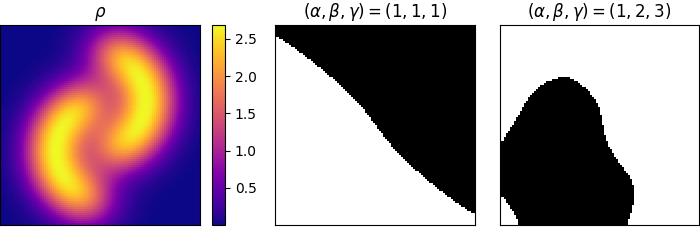
\includegraphics[width=4.5in]{images/moons.png}
}\hspace{0mm}
\subfloat[Noisy concentric circles]{
  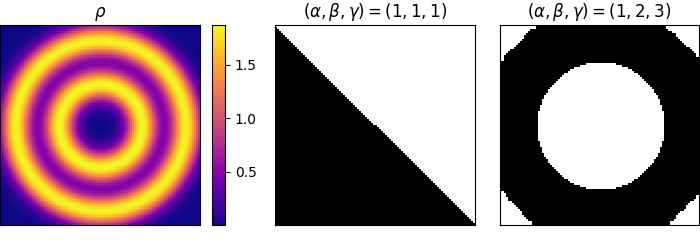
\includegraphics[width=4.5in]{images/circles.png}
}\hspace{0mm}
\subfloat[Long valley]{
  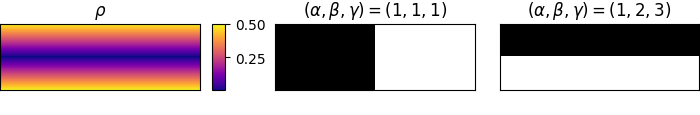
\includegraphics[width=4.5in]{images/trough.png}
}
\caption{
In each row, the first image shows the heat map of a fixed $\rho:\Omega\to\RR_>0$, the second and third images shows the set $\Omega_k$ returned by Algorithm \ref{alg:multiple_cuts} (displayed in black) for the choices $(\alpha,\beta,\gamma)$ of $(1,1,1)$ and $(1,2,3)$ respectively.
 }
\label{fig:alg}
\end{figure}



\unappendix
\end{appendix}



%\end{document}
